% Options for packages loaded elsewhere
\PassOptionsToPackage{unicode}{hyperref}
\PassOptionsToPackage{hyphens}{url}
%
\documentclass[
]{book}
\usepackage{amsmath,amssymb}
\usepackage{iftex}
\ifPDFTeX
  \usepackage[T1]{fontenc}
  \usepackage[utf8]{inputenc}
  \usepackage{textcomp} % provide euro and other symbols
\else % if luatex or xetex
  \usepackage{unicode-math} % this also loads fontspec
  \defaultfontfeatures{Scale=MatchLowercase}
  \defaultfontfeatures[\rmfamily]{Ligatures=TeX,Scale=1}
\fi
\usepackage{lmodern}
\ifPDFTeX\else
  % xetex/luatex font selection
\fi
% Use upquote if available, for straight quotes in verbatim environments
\IfFileExists{upquote.sty}{\usepackage{upquote}}{}
\IfFileExists{microtype.sty}{% use microtype if available
  \usepackage[]{microtype}
  \UseMicrotypeSet[protrusion]{basicmath} % disable protrusion for tt fonts
}{}
\makeatletter
\@ifundefined{KOMAClassName}{% if non-KOMA class
  \IfFileExists{parskip.sty}{%
    \usepackage{parskip}
  }{% else
    \setlength{\parindent}{0pt}
    \setlength{\parskip}{6pt plus 2pt minus 1pt}}
}{% if KOMA class
  \KOMAoptions{parskip=half}}
\makeatother
\usepackage{xcolor}
\usepackage{color}
\usepackage{fancyvrb}
\newcommand{\VerbBar}{|}
\newcommand{\VERB}{\Verb[commandchars=\\\{\}]}
\DefineVerbatimEnvironment{Highlighting}{Verbatim}{commandchars=\\\{\}}
% Add ',fontsize=\small' for more characters per line
\usepackage{framed}
\definecolor{shadecolor}{RGB}{248,248,248}
\newenvironment{Shaded}{\begin{snugshade}}{\end{snugshade}}
\newcommand{\AlertTok}[1]{\textcolor[rgb]{0.94,0.16,0.16}{#1}}
\newcommand{\AnnotationTok}[1]{\textcolor[rgb]{0.56,0.35,0.01}{\textbf{\textit{#1}}}}
\newcommand{\AttributeTok}[1]{\textcolor[rgb]{0.13,0.29,0.53}{#1}}
\newcommand{\BaseNTok}[1]{\textcolor[rgb]{0.00,0.00,0.81}{#1}}
\newcommand{\BuiltInTok}[1]{#1}
\newcommand{\CharTok}[1]{\textcolor[rgb]{0.31,0.60,0.02}{#1}}
\newcommand{\CommentTok}[1]{\textcolor[rgb]{0.56,0.35,0.01}{\textit{#1}}}
\newcommand{\CommentVarTok}[1]{\textcolor[rgb]{0.56,0.35,0.01}{\textbf{\textit{#1}}}}
\newcommand{\ConstantTok}[1]{\textcolor[rgb]{0.56,0.35,0.01}{#1}}
\newcommand{\ControlFlowTok}[1]{\textcolor[rgb]{0.13,0.29,0.53}{\textbf{#1}}}
\newcommand{\DataTypeTok}[1]{\textcolor[rgb]{0.13,0.29,0.53}{#1}}
\newcommand{\DecValTok}[1]{\textcolor[rgb]{0.00,0.00,0.81}{#1}}
\newcommand{\DocumentationTok}[1]{\textcolor[rgb]{0.56,0.35,0.01}{\textbf{\textit{#1}}}}
\newcommand{\ErrorTok}[1]{\textcolor[rgb]{0.64,0.00,0.00}{\textbf{#1}}}
\newcommand{\ExtensionTok}[1]{#1}
\newcommand{\FloatTok}[1]{\textcolor[rgb]{0.00,0.00,0.81}{#1}}
\newcommand{\FunctionTok}[1]{\textcolor[rgb]{0.13,0.29,0.53}{\textbf{#1}}}
\newcommand{\ImportTok}[1]{#1}
\newcommand{\InformationTok}[1]{\textcolor[rgb]{0.56,0.35,0.01}{\textbf{\textit{#1}}}}
\newcommand{\KeywordTok}[1]{\textcolor[rgb]{0.13,0.29,0.53}{\textbf{#1}}}
\newcommand{\NormalTok}[1]{#1}
\newcommand{\OperatorTok}[1]{\textcolor[rgb]{0.81,0.36,0.00}{\textbf{#1}}}
\newcommand{\OtherTok}[1]{\textcolor[rgb]{0.56,0.35,0.01}{#1}}
\newcommand{\PreprocessorTok}[1]{\textcolor[rgb]{0.56,0.35,0.01}{\textit{#1}}}
\newcommand{\RegionMarkerTok}[1]{#1}
\newcommand{\SpecialCharTok}[1]{\textcolor[rgb]{0.81,0.36,0.00}{\textbf{#1}}}
\newcommand{\SpecialStringTok}[1]{\textcolor[rgb]{0.31,0.60,0.02}{#1}}
\newcommand{\StringTok}[1]{\textcolor[rgb]{0.31,0.60,0.02}{#1}}
\newcommand{\VariableTok}[1]{\textcolor[rgb]{0.00,0.00,0.00}{#1}}
\newcommand{\VerbatimStringTok}[1]{\textcolor[rgb]{0.31,0.60,0.02}{#1}}
\newcommand{\WarningTok}[1]{\textcolor[rgb]{0.56,0.35,0.01}{\textbf{\textit{#1}}}}
\usepackage{longtable,booktabs,array}
\usepackage{calc} % for calculating minipage widths
% Correct order of tables after \paragraph or \subparagraph
\usepackage{etoolbox}
\makeatletter
\patchcmd\longtable{\par}{\if@noskipsec\mbox{}\fi\par}{}{}
\makeatother
% Allow footnotes in longtable head/foot
\IfFileExists{footnotehyper.sty}{\usepackage{footnotehyper}}{\usepackage{footnote}}
\makesavenoteenv{longtable}
\usepackage{graphicx}
\makeatletter
\def\maxwidth{\ifdim\Gin@nat@width>\linewidth\linewidth\else\Gin@nat@width\fi}
\def\maxheight{\ifdim\Gin@nat@height>\textheight\textheight\else\Gin@nat@height\fi}
\makeatother
% Scale images if necessary, so that they will not overflow the page
% margins by default, and it is still possible to overwrite the defaults
% using explicit options in \includegraphics[width, height, ...]{}
\setkeys{Gin}{width=\maxwidth,height=\maxheight,keepaspectratio}
% Set default figure placement to htbp
\makeatletter
\def\fps@figure{htbp}
\makeatother
\setlength{\emergencystretch}{3em} % prevent overfull lines
\providecommand{\tightlist}{%
  \setlength{\itemsep}{0pt}\setlength{\parskip}{0pt}}
\setcounter{secnumdepth}{5}
\usepackage{booktabs}
\usepackage{amsthm}
\makeatletter
\def\thm@space@setup{%
  \thm@preskip=8pt plus 2pt minus 4pt
  \thm@postskip=\thm@preskip
}
\makeatother
\ifLuaTeX
  \usepackage{selnolig}  % disable illegal ligatures
\fi
\usepackage[]{natbib}
\bibliographystyle{apalike}
\usepackage{bookmark}
\IfFileExists{xurl.sty}{\usepackage{xurl}}{} % add URL line breaks if available
\urlstyle{same}
\hypersetup{
  pdftitle={{[}PSY202A Lab{]} Statistical Modeling in Psychological Sciences},
  pdfauthor={Ihnwhi Heo, M.Sc.},
  hidelinks,
  pdfcreator={LaTeX via pandoc}}

\title{{[}PSY202A Lab{]} Statistical Modeling in Psychological Sciences}
\author{\href{https://ihnwhiheo.github.io/}{Ihnwhi Heo, M.Sc.}}
\date{Fall 2024}

\begin{document}
\maketitle

{
\setcounter{tocdepth}{1}
\tableofcontents
}
\chapter{Introduction}\label{introduction}

Hi everyone! I'm Ihnwhi.

It is my great pleasure to be your guest lecturer for PSY202A.

Statistical modeling is a key component in conducting research in the psychological sciences. While many statistical toolkits are available to researchers, R is arguably one of the most useful free and open-source statistical software programs. It offers a dizzying array of analytic options to answer your important and exciting research questions. In the upcoming four lab sessions, you will be introduced to R and become familiar with its capabilities. These sessions are designed to help you get acquainted with the fundamentals of R and learn how to use it wisely as the next generation of psychologists. You will then be guided through summarizing and analyzing data using R.

I must acknowledge that these materials are the result of the dedication and efforts of many remarkable researchers who have contributed to improving statistics resources. These include Fan Jia, Marieke Visser, Luca Marvin, Terrence Jorgensen, and Sunthud Pornprasertmanit.

Are you ready? Let's get it on!

\chapter{Introduction to R: Part 1}\label{introduction-to-r-part-1}

\section{Word of wisdom}\label{word-of-wisdom}

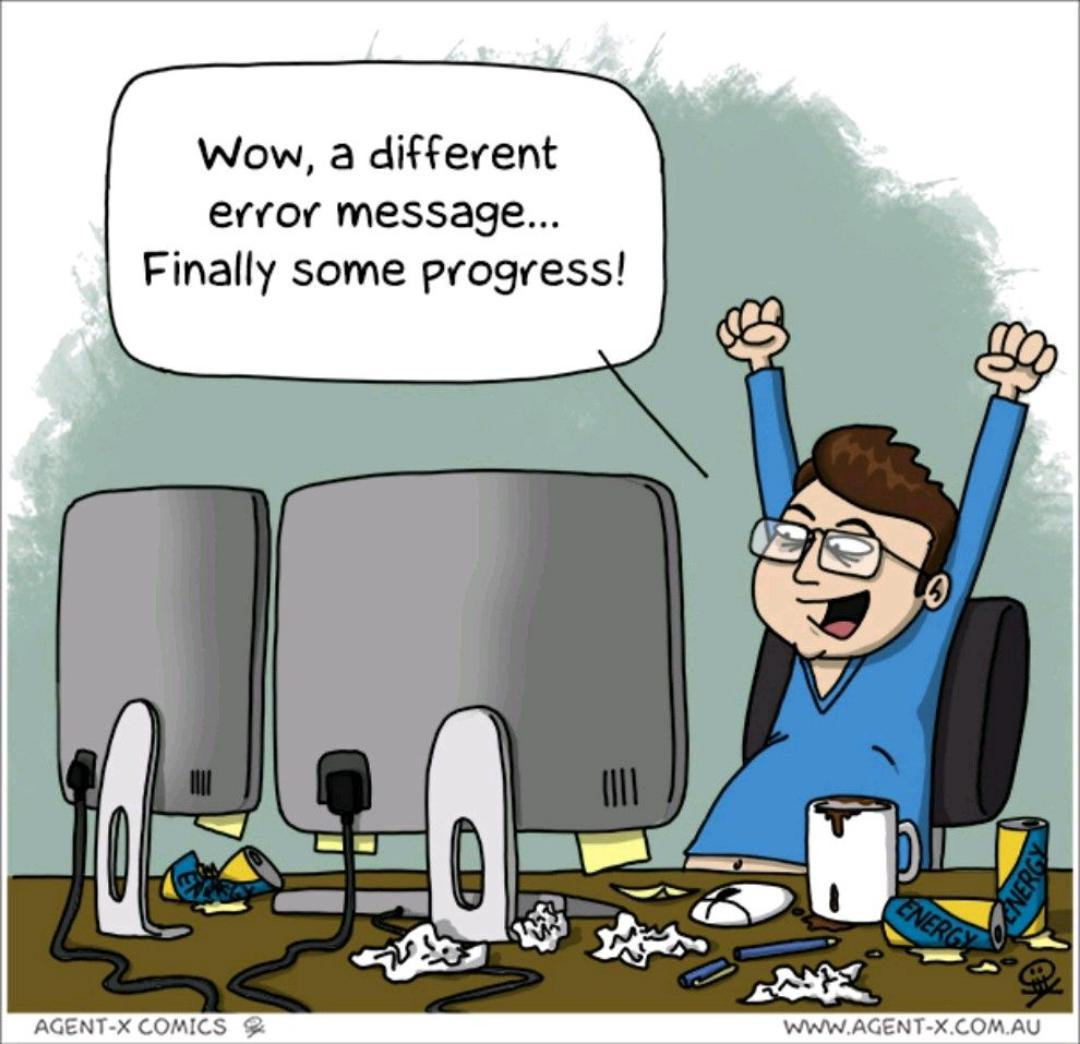
\includegraphics{./img/programming_meme.jpg}

\begin{itemize}
\item
  Don't worry about making mistakes; it's part of the process.
\item
  Feel free to ask questions to me or your peers.
\item
  Remember, there isn't just one way to solve a problem.
\item
  Be a wise user of resources like Google, YouTube, or AI.
\item
  Keep in mind that you're not the only one struggling.
\end{itemize}

\section{How R you?}\label{how-r-you}

\subsection{Open RStudio}\label{open-rstudio}

\begin{itemize}
\tightlist
\item
  Can you find three panes?
\end{itemize}

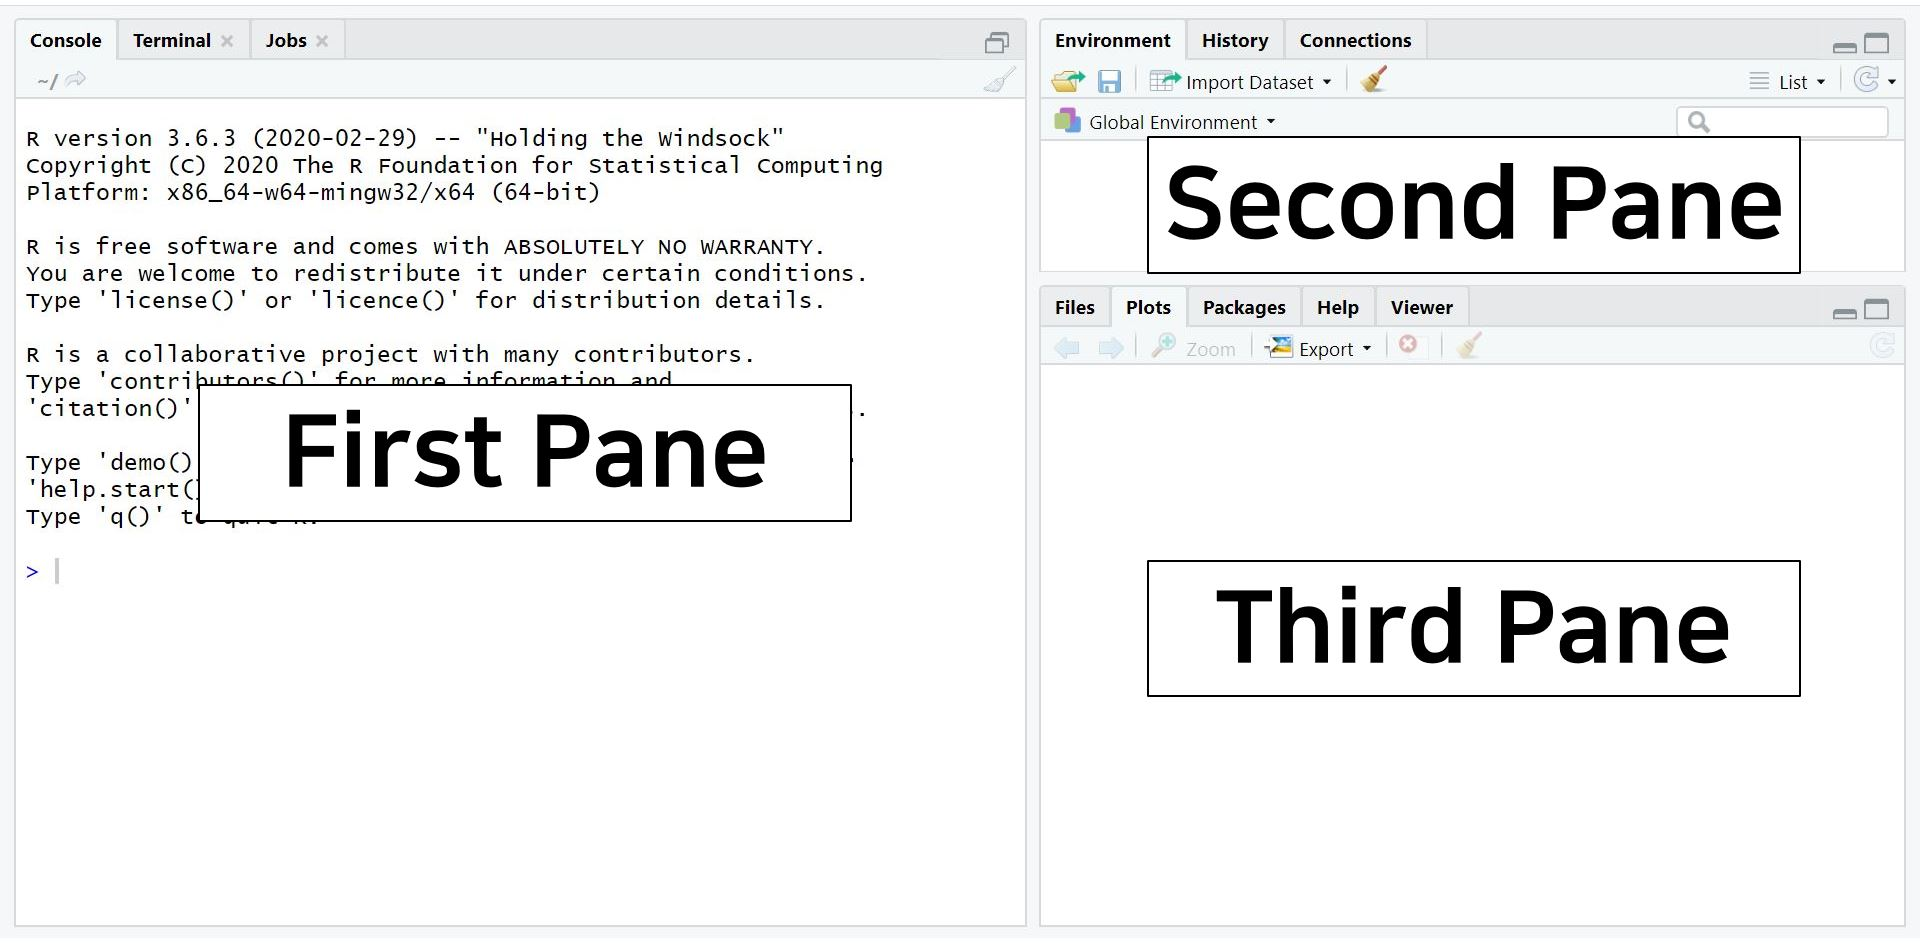
\includegraphics{./img/first_glance.jpg}

\subsection{Open a new R script}\label{open-a-new-r-script}

\begin{itemize}
\tightlist
\item
  Can you find four panes?
\end{itemize}

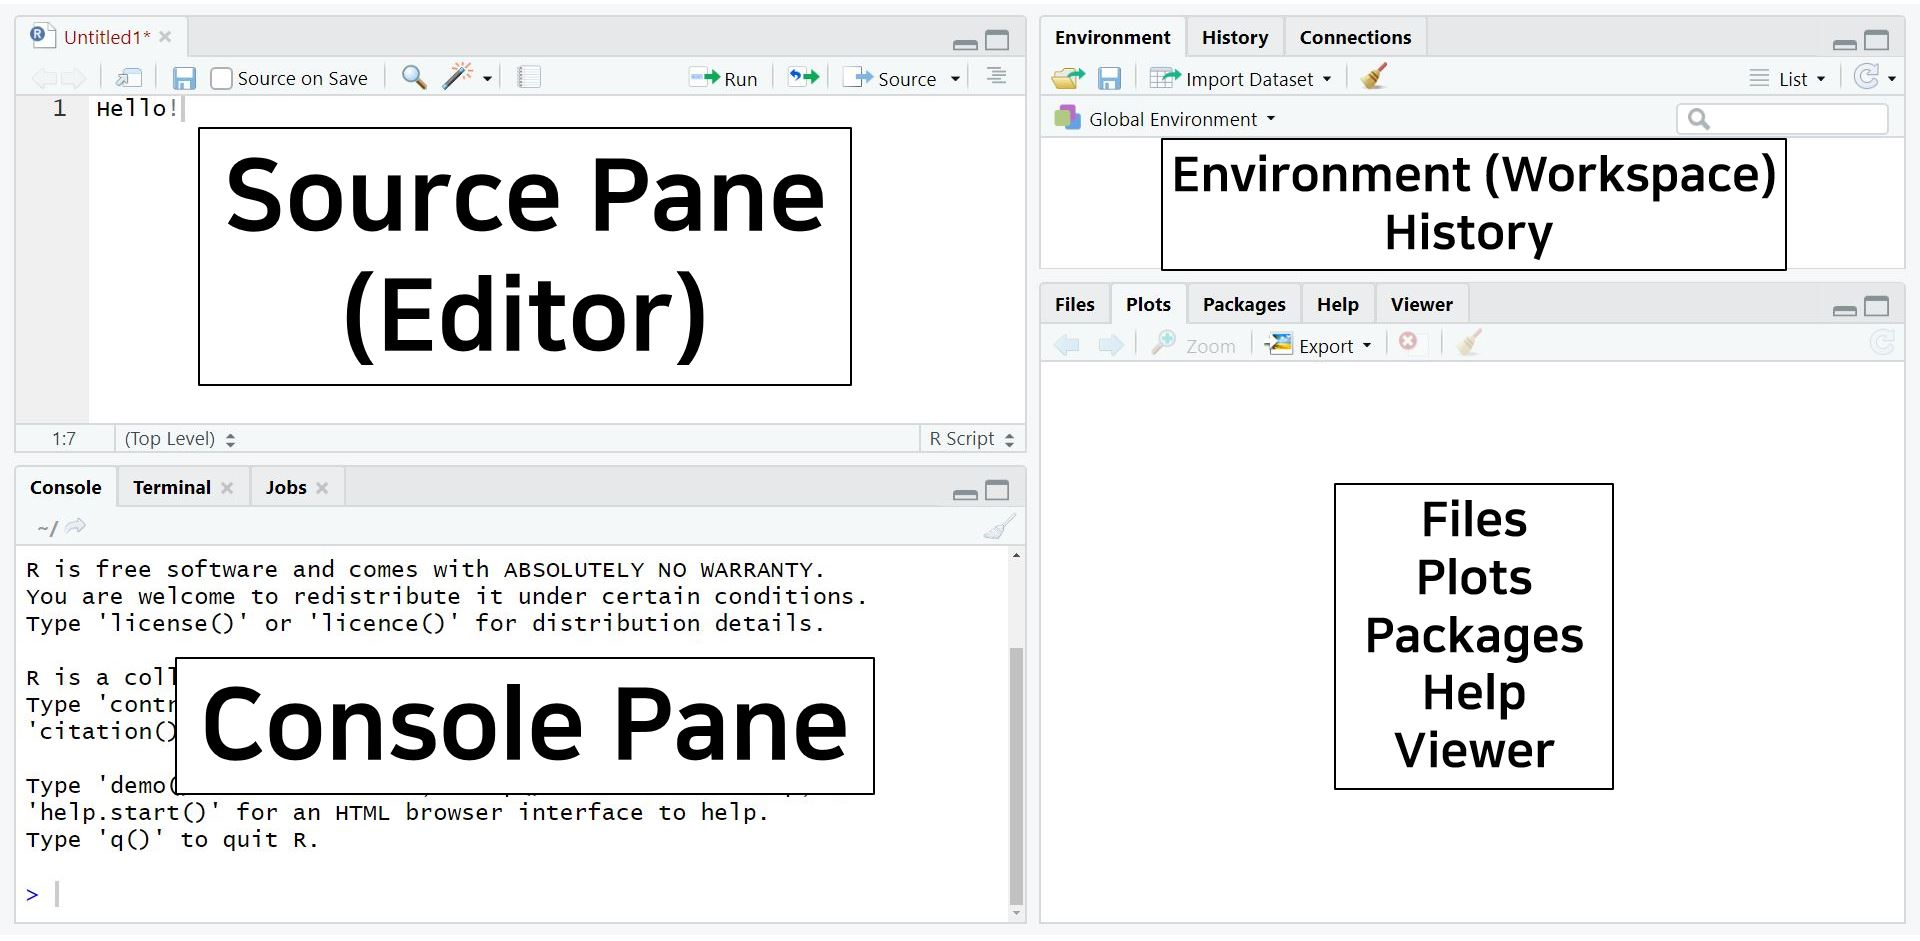
\includegraphics{./img/second_glance.jpg}

\subsection{Individualize R}\label{individualize-r}

\begin{itemize}
\tightlist
\item
  Can you find your own R style?
\end{itemize}

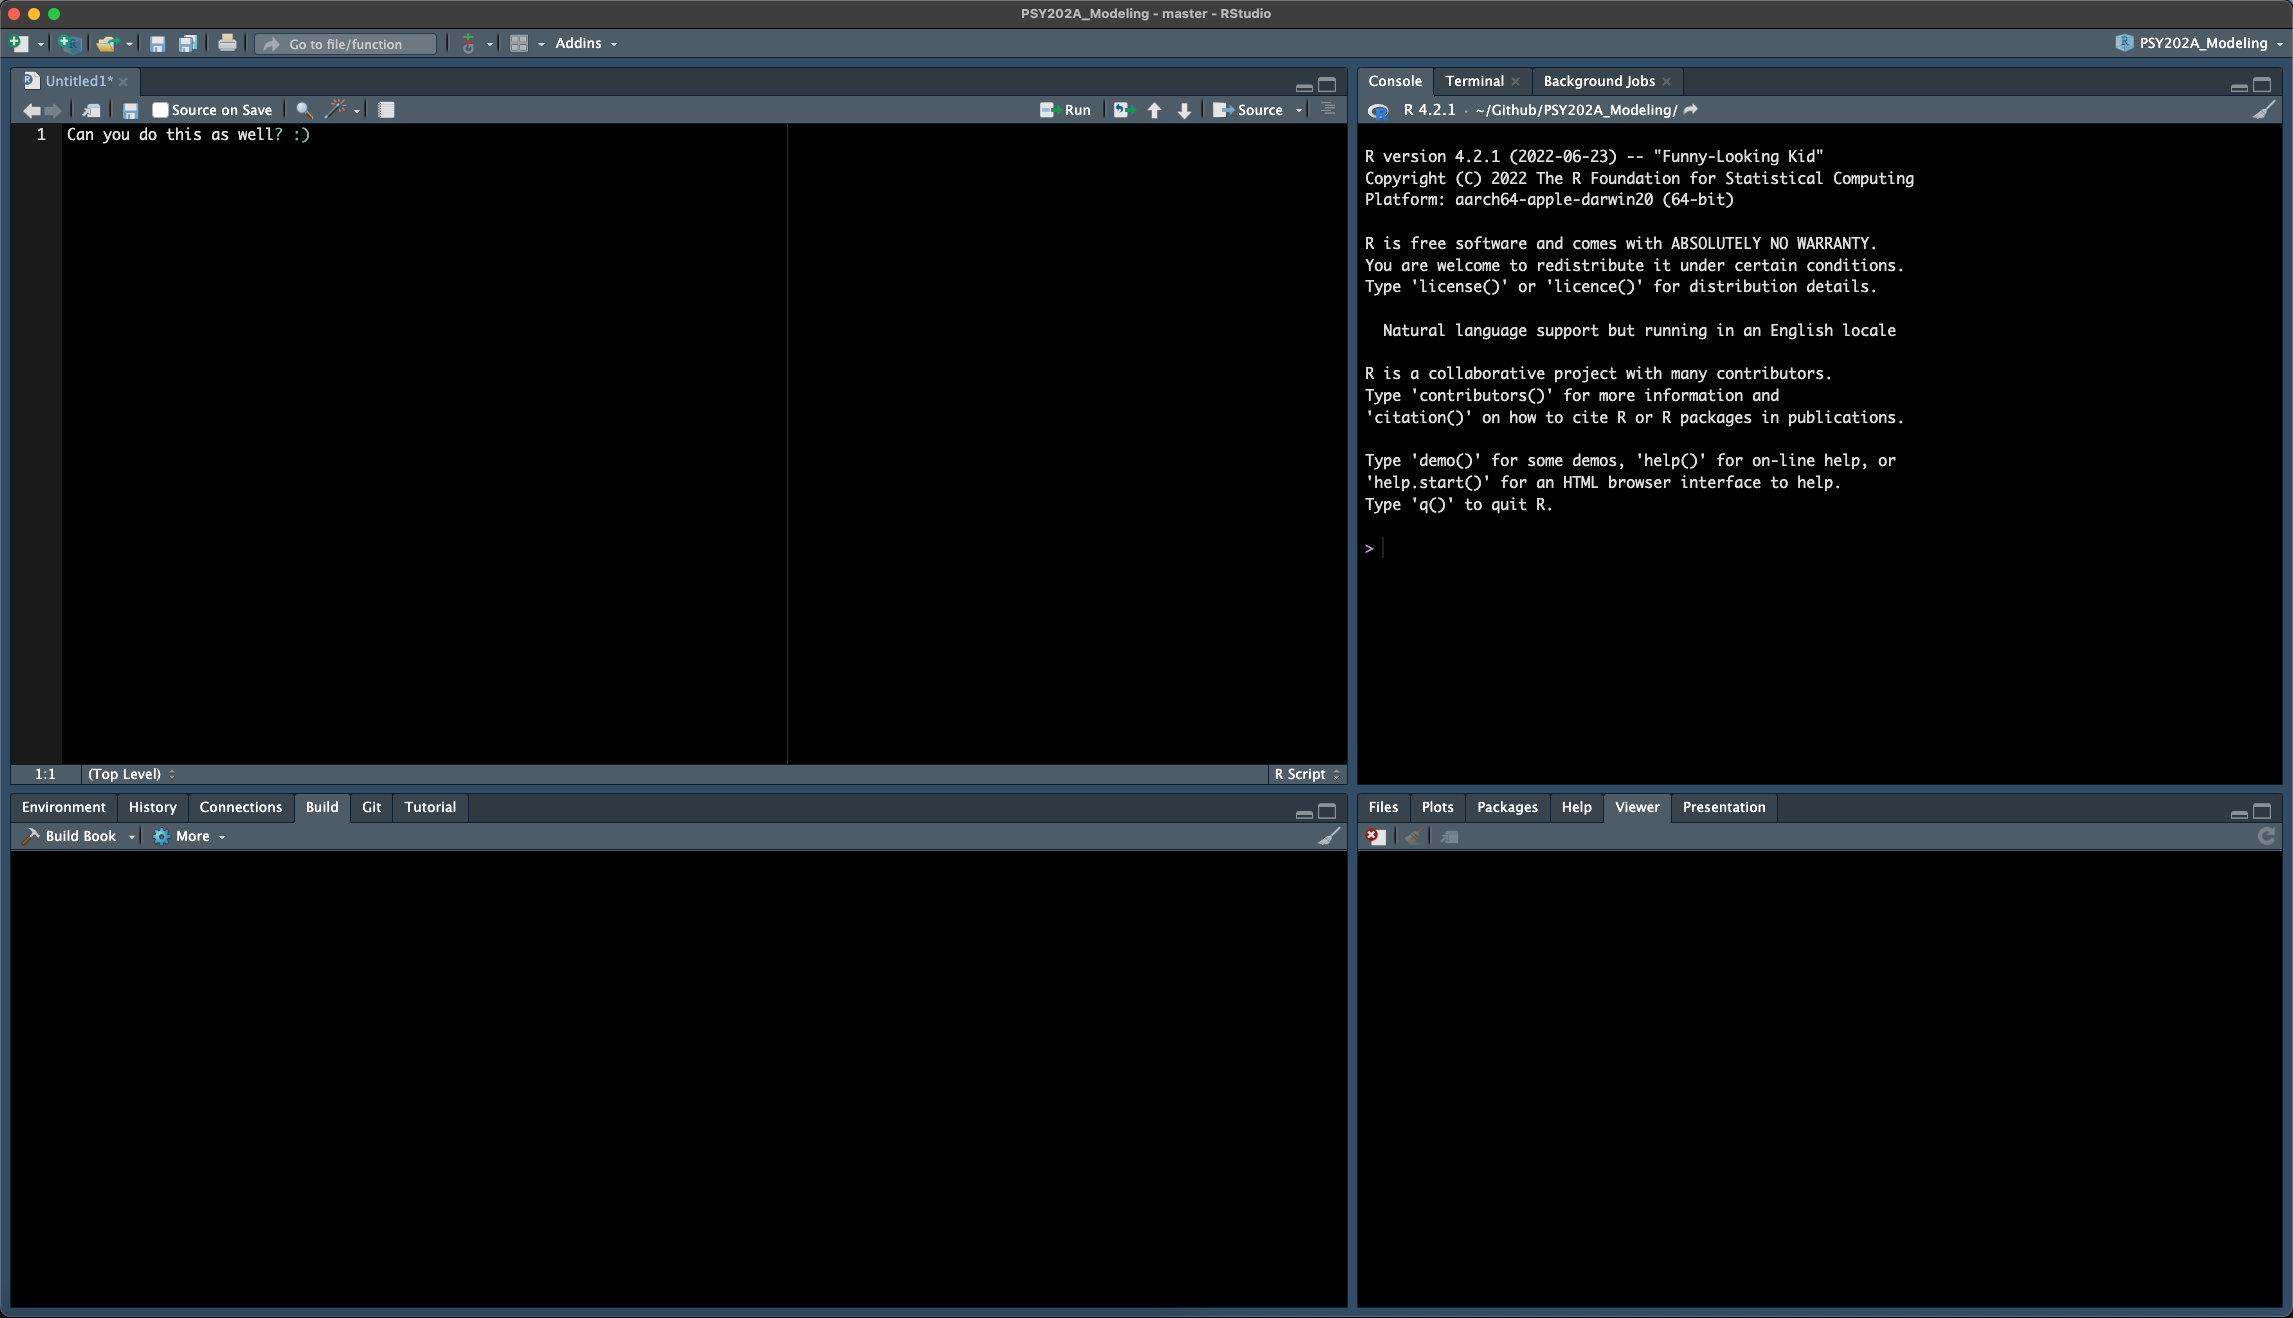
\includegraphics{./img/third_glance.png}

\subsection{Some useful settings}\label{some-useful-settings}

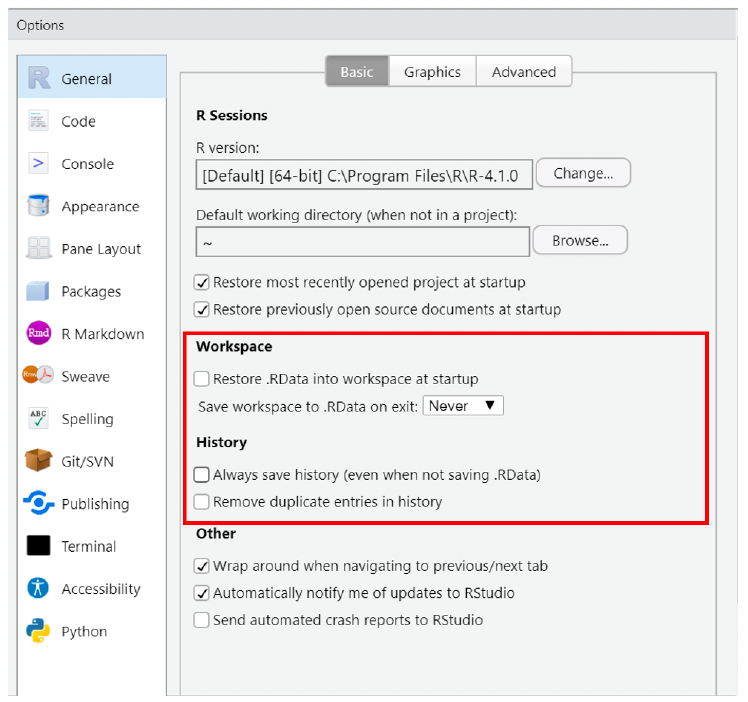
\includegraphics{./img/useful_settings.png}

\begin{itemize}
\tightlist
\item
  Under ``Workspace'':

  \begin{itemize}
  \tightlist
  \item
    Uncheck restore .RData into workspace at startup.
  \item
    Save workshop to .Rdata on exit: ``Never''.
  \end{itemize}
\item
  Under ``History'':

  \begin{itemize}
  \tightlist
  \item
    Uncheck ``Always save history (even when not saving .RData).
  \item
    Uncheck ``Remove duplicate entries in history''.
  \end{itemize}
\end{itemize}

\section{Interacting with R}\label{interacting-with-r}

\begin{itemize}
\tightlist
\item
  How to run R commands?

  \begin{itemize}
  \tightlist
  \item
    Put your cursor on a line, or select the line(s), hit the Run button.
  \item
    The hot key for Run the current line'selection is Ctrl + Enter (Windoes) or Command + Return (Mac).
  \end{itemize}
\item
  Can you run the below code?
\end{itemize}

\begin{Shaded}
\begin{Highlighting}[]
\NormalTok{greetings }\OtherTok{\textless{}{-}} \StringTok{"Hello PSY202A"}
\FunctionTok{print}\NormalTok{(greetings)}
\end{Highlighting}
\end{Shaded}

\begin{itemize}
\item
  Everything starting with a pound sign (\#) is considered as a comment. R will skep all the characters after \# until it finds a new line of command.
\item
  Can you run the below code?
\end{itemize}

\begin{Shaded}
\begin{Highlighting}[]
\NormalTok{Comment}

\CommentTok{\# Comment}
\end{Highlighting}
\end{Shaded}

\section{Computation}\label{computation}

\subsection{Using R as a numerical calculator}\label{using-r-as-a-numerical-calculator}

\begin{itemize}
\tightlist
\item
  Can you run the code below?
\end{itemize}

\begin{Shaded}
\begin{Highlighting}[]
\DecValTok{2} \SpecialCharTok{+} \DecValTok{4} \CommentTok{\# Addition}
\DecValTok{2} \SpecialCharTok{{-}} \DecValTok{4} \CommentTok{\# Subtraction}
\DecValTok{2} \SpecialCharTok{*} \DecValTok{4} \CommentTok{\# Multiplication}
\DecValTok{2} \SpecialCharTok{/} \DecValTok{4} \CommentTok{\# Division}
\DecValTok{2} \SpecialCharTok{**} \DecValTok{4} \CommentTok{\# Power}
\FunctionTok{sqrt}\NormalTok{(}\DecValTok{144}\NormalTok{) }\CommentTok{\# Square root}
\FunctionTok{log}\NormalTok{(}\DecValTok{144}\NormalTok{) }\CommentTok{\# Natural logarithm}
\FunctionTok{exp}\NormalTok{(}\DecValTok{5}\NormalTok{) }\CommentTok{\# Exponential, i.e., power of e}
\NormalTok{(}\DecValTok{10} \SpecialCharTok{+} \DecValTok{2}\SpecialCharTok{*}\FunctionTok{log}\NormalTok{(}\DecValTok{8}\NormalTok{) }\SpecialCharTok{{-}}\NormalTok{ (}\FunctionTok{exp}\NormalTok{(}\DecValTok{8}\NormalTok{) }\SpecialCharTok{{-}} \DecValTok{4}\NormalTok{)}\SpecialCharTok{/}\DecValTok{3}\NormalTok{) }\SpecialCharTok{*} \DecValTok{7}
\end{Highlighting}
\end{Shaded}

\begin{itemize}
\tightlist
\item
  Here, \texttt{sqrt()}, \texttt{log()}, and \texttt{exp()} are numerical functions.
\end{itemize}

\subsubsection{Exercise: Numerical calculator}\label{exercise-numerical-calculator}

\begin{itemize}
\tightlist
\item
  Can you give me the answer to the mathematical formula below?
\end{itemize}

\[
\frac{26}{\text{log}(5)}\times e^{3} + (-0.2)
\]

\begin{itemize}
\tightlist
\item
  How about this?
\end{itemize}

\[
-\sqrt( \text{ln}7 )
\]

\subsection{Using R as a logical calculator}\label{using-r-as-a-logical-calculator}

\begin{itemize}
\tightlist
\item
  You can also use R for logical statements.
\end{itemize}

\begin{Shaded}
\begin{Highlighting}[]
\DecValTok{1} \SpecialCharTok{==} \DecValTok{1} \CommentTok{\# equal}
\DecValTok{1} \SpecialCharTok{!=} \DecValTok{2} \CommentTok{\# unequal}
\DecValTok{10} \SpecialCharTok{\textgreater{}} \DecValTok{1} \CommentTok{\# greater than}
\DecValTok{10} \SpecialCharTok{\textgreater{}=} \DecValTok{1} \CommentTok{\# greater than or equal to}
\end{Highlighting}
\end{Shaded}

\subsubsection{Exercise: Logical calculator}\label{exercise-logical-calculator}

\begin{itemize}
\tightlist
\item
  Then\ldots{} can you program your code to evaluate the below statements?

  \begin{itemize}
  \tightlist
  \item
    Try this first: 5 is lower than or equal to 10. What is the result? Does this make sense?
  \item
    Then, try this second: 10 is not equal to 10. What is the result? Does this make sense?
  \end{itemize}
\end{itemize}

\section{Types of objects}\label{types-of-objects}

\begin{itemize}
\tightlist
\item
  In R, anything with a name is an object.

  \begin{itemize}
  \tightlist
  \item
    You can give an object with any name you want insofar as that name is not taken in R already.
  \end{itemize}
\item
  An object can contain more than one value and have more complex data strutures, such as:

  \begin{itemize}
  \tightlist
  \item
    vector: a series of values of the same data type
  \item
    matrix: a two-dimensional table of values with the same data type
  \item
    data frame: a two-dimensional table of values, may not be the same data type
  \item
    list: an object made of objects
  \end{itemize}
\end{itemize}

\subsection{Vector: Intro}\label{vector-intro}

\begin{itemize}
\tightlist
\item
  The concatenate function \texttt{c()} is usually used to put a set of values together.

  \begin{itemize}
  \tightlist
  \item
    An object \texttt{iq} is a vector of 5 IQ scores.
  \end{itemize}
\end{itemize}

\begin{Shaded}
\begin{Highlighting}[]
\CommentTok{\# A vector of IQ scores}
\NormalTok{iq }\OtherTok{\textless{}{-}} \FunctionTok{c}\NormalTok{(}\DecValTok{90}\NormalTok{, }\DecValTok{100}\NormalTok{, }\DecValTok{105}\NormalTok{, }\DecValTok{110}\NormalTok{, }\DecValTok{95}\NormalTok{)}

\CommentTok{\# Here, \textquotesingle{}iq\textquotesingle{} is an object}

\CommentTok{\# Print the IQ object}
\FunctionTok{print}\NormalTok{(iq)}
\NormalTok{iq}
\end{Highlighting}
\end{Shaded}

\begin{itemize}
\tightlist
\item
  Out of curiosity, what should we do if we want to know the sum of all the five iq scores? You can use the \texttt{sum()} function. Can you try?
\end{itemize}

\begin{Shaded}
\begin{Highlighting}[]
\CommentTok{\# Hint: put an object name within the sum()}
\end{Highlighting}
\end{Shaded}

\begin{itemize}
\tightlist
\item
  Many other functions also return vectors as results.

  \begin{itemize}
  \tightlist
  \item
    For instance, the sequence operator (:) generates consecutive numbers.
  \end{itemize}
\end{itemize}

\begin{Shaded}
\begin{Highlighting}[]
\NormalTok{numbers }\OtherTok{\textless{}{-}} \DecValTok{1}\SpecialCharTok{:}\DecValTok{100}
\NormalTok{numbers}
\end{Highlighting}
\end{Shaded}

\subsubsection{Exercise: Vector intro}\label{exercise-vector-intro}

\begin{itemize}
\tightlist
\item
  There are other specific functions. Can you guess what each of the functions does?
\end{itemize}

\begin{Shaded}
\begin{Highlighting}[]
\CommentTok{\# Describe what the below function does: }
\NormalTok{values\_1 }\OtherTok{\textless{}{-}} \FunctionTok{seq}\NormalTok{(}\DecValTok{1}\NormalTok{, }\DecValTok{5}\NormalTok{, }\AttributeTok{by =} \DecValTok{1}\NormalTok{)}

\CommentTok{\# Describe what the below function does: }
\NormalTok{values\_2 }\OtherTok{\textless{}{-}} \FunctionTok{seq}\NormalTok{(}\DecValTok{1}\NormalTok{, }\DecValTok{5}\NormalTok{, }\AttributeTok{by =} \FloatTok{0.5}\NormalTok{)}

\CommentTok{\# Describe what the below function does: }
\NormalTok{values\_3 }\OtherTok{\textless{}{-}} \FunctionTok{rep}\NormalTok{(}\DecValTok{1}\NormalTok{, }\DecValTok{5}\NormalTok{)}

\CommentTok{\# Describe what the below function does: }
\NormalTok{values\_4 }\OtherTok{\textless{}{-}} \FunctionTok{rep}\NormalTok{(}\DecValTok{1}\SpecialCharTok{:}\DecValTok{5}\NormalTok{, }\DecValTok{3}\NormalTok{)}
\end{Highlighting}
\end{Shaded}

\subsection{Vector: Advanced}\label{vector-advanced}

\begin{itemize}
\item
  There are a couple of distribution functions that can be used to generate a vector of random numbers from a specific distribution.
\item
  For example, you can generate 5 random numbers from a normal distribution with a mean of 0 and a standard deviation of 1:
\end{itemize}

\begin{Shaded}
\begin{Highlighting}[]
\NormalTok{random\_normal }\OtherTok{\textless{}{-}} \FunctionTok{rnorm}\NormalTok{(}\DecValTok{5}\NormalTok{, }\DecValTok{0}\NormalTok{, }\DecValTok{1}\NormalTok{)}
\NormalTok{random\_normal}
\end{Highlighting}
\end{Shaded}

\begin{itemize}
\tightlist
\item
  As another example, you can generate 5 random numbers from a uniform distribution between 0 and 1:
\end{itemize}

\begin{Shaded}
\begin{Highlighting}[]
\NormalTok{random\_uniform }\OtherTok{\textless{}{-}} \FunctionTok{runif}\NormalTok{(}\DecValTok{5}\NormalTok{, }\DecValTok{0}\NormalTok{, }\DecValTok{1}\NormalTok{)}
\NormalTok{random\_uniform}
\end{Highlighting}
\end{Shaded}

\begin{itemize}
\tightlist
\item
  The standard arithmetic operators and functions apply to vectors on a element-wise basis.
\end{itemize}

\begin{Shaded}
\begin{Highlighting}[]
\NormalTok{A }\OtherTok{\textless{}{-}} \FunctionTok{c}\NormalTok{(}\DecValTok{1}\NormalTok{, }\DecValTok{2}\NormalTok{, }\DecValTok{3}\NormalTok{, }\DecValTok{4}\NormalTok{) }\SpecialCharTok{{-}} \DecValTok{4}
\NormalTok{A}

\NormalTok{B }\OtherTok{\textless{}{-}} \FunctionTok{c}\NormalTok{(}\DecValTok{1}\NormalTok{, }\DecValTok{2}\NormalTok{, }\DecValTok{3}\NormalTok{, }\DecValTok{4}\NormalTok{)}\SpecialCharTok{/}\DecValTok{4}
\NormalTok{B}

\NormalTok{C }\OtherTok{\textless{}{-}} \FunctionTok{c}\NormalTok{(}\DecValTok{1}\NormalTok{, }\DecValTok{2}\NormalTok{, }\DecValTok{3}\NormalTok{, }\DecValTok{4}\NormalTok{)}\SpecialCharTok{/}\FunctionTok{c}\NormalTok{(}\DecValTok{4}\NormalTok{, }\DecValTok{3}\NormalTok{, }\DecValTok{2}\NormalTok{, }\DecValTok{1}\NormalTok{)}
\NormalTok{C}

\NormalTok{D }\OtherTok{\textless{}{-}} \FunctionTok{log}\NormalTok{(}\FunctionTok{c}\NormalTok{(}\DecValTok{1}\NormalTok{, }\DecValTok{2}\NormalTok{, }\DecValTok{3}\NormalTok{, }\DecValTok{4}\NormalTok{))}
\NormalTok{D}
\end{Highlighting}
\end{Shaded}

\begin{itemize}
\tightlist
\item
  All elements in a vector must be the same type

  \begin{itemize}
  \tightlist
  \item
    Numeric, character (aka. string), logic
  \end{itemize}
\end{itemize}

\begin{Shaded}
\begin{Highlighting}[]
\NormalTok{numeric\_vector }\OtherTok{\textless{}{-}} \FunctionTok{c}\NormalTok{(}\DecValTok{1}\NormalTok{, }\DecValTok{2}\NormalTok{, }\DecValTok{3}\NormalTok{, }\DecValTok{4}\NormalTok{)}

\NormalTok{character\_vector }\OtherTok{\textless{}{-}} \FunctionTok{c}\NormalTok{(}\StringTok{"developmental"}\NormalTok{, }\StringTok{"health"}\NormalTok{, }\StringTok{"quantitative"}\NormalTok{)}

\NormalTok{logical\_vector }\OtherTok{\textless{}{-}} \FunctionTok{c}\NormalTok{(}\ConstantTok{FALSE}\NormalTok{, }\ConstantTok{TRUE}\NormalTok{, }\ConstantTok{FALSE}\NormalTok{, }\ConstantTok{FALSE}\NormalTok{)}
\end{Highlighting}
\end{Shaded}

\subsubsection{Exercise: Vector advanced}\label{exercise-vector-advanced}

Can you run the code below? What do you see?

\begin{Shaded}
\begin{Highlighting}[]
\NormalTok{numeric\_vector}\SpecialCharTok{\^{}}\DecValTok{2}

\DecValTok{1}\SpecialCharTok{/}\NormalTok{numeric\_vector}

\NormalTok{numeric\_vector }\SpecialCharTok{+}\NormalTok{ character\_vector}

\NormalTok{character\_vector }\SpecialCharTok{+}\NormalTok{ logical\_vector}

\NormalTok{numeric\_vector }\SpecialCharTok{+}\NormalTok{ logical\_vector}

\NormalTok{logical\_vector }\SpecialCharTok{+}\NormalTok{ logical\_vector}

\NormalTok{logical\_vector}\SpecialCharTok{+}\DecValTok{5}
\end{Highlighting}
\end{Shaded}

\subsection{Matrix: intro}\label{matrix-intro}

\begin{itemize}
\tightlist
\item
  We can create a matrix by combining multiple vectors (e.g., perhaps associated with multiple scales)
\end{itemize}

\begin{Shaded}
\begin{Highlighting}[]
\NormalTok{scale1 }\OtherTok{\textless{}{-}} \FunctionTok{c}\NormalTok{(}\DecValTok{1}\NormalTok{, }\DecValTok{4}\NormalTok{, }\DecValTok{7}\NormalTok{, }\DecValTok{4}\NormalTok{, }\DecValTok{5}\NormalTok{)}
\NormalTok{scale2 }\OtherTok{\textless{}{-}} \FunctionTok{c}\NormalTok{(}\DecValTok{5}\NormalTok{, }\DecValTok{6}\NormalTok{, }\DecValTok{8}\NormalTok{, }\DecValTok{3}\NormalTok{, }\DecValTok{2}\NormalTok{)}
\NormalTok{scale3 }\OtherTok{\textless{}{-}} \FunctionTok{c}\NormalTok{(}\DecValTok{0}\NormalTok{, }\DecValTok{9}\NormalTok{, }\DecValTok{8}\NormalTok{, }\DecValTok{9}\NormalTok{, }\DecValTok{3}\NormalTok{)}
\end{Highlighting}
\end{Shaded}

\begin{itemize}
\tightlist
\item
  We could arrange these into a table, using \texttt{cbind()} function (bind by column).
\end{itemize}

\begin{Shaded}
\begin{Highlighting}[]
\NormalTok{my\_data }\OtherTok{\textless{}{-}} \FunctionTok{cbind}\NormalTok{(scale1, scale2, scale3)}
\NormalTok{my\_data}
\end{Highlighting}
\end{Shaded}

\begin{itemize}
\tightlist
\item
  Or, if our data were in one long vector:
\end{itemize}

\begin{Shaded}
\begin{Highlighting}[]
\NormalTok{long\_vec }\OtherTok{\textless{}{-}} \FunctionTok{c}\NormalTok{(scale1, scale2, scale3)}
\NormalTok{my\_matrix }\OtherTok{\textless{}{-}} \FunctionTok{matrix}\NormalTok{(long\_vec, }\AttributeTok{ncol =} \DecValTok{3}\NormalTok{, }\AttributeTok{byrow =} \ConstantTok{FALSE}\NormalTok{)}
\NormalTok{my\_matrix}
\end{Highlighting}
\end{Shaded}

\subsection{Matrix: advanced}\label{matrix-advanced}

\begin{itemize}
\tightlist
\item
  Find the size of the matrix (i.e., the number of rows and the number of columns) using \texttt{dim()}:
\end{itemize}

\begin{Shaded}
\begin{Highlighting}[]
\FunctionTok{dim}\NormalTok{(my\_matrix)}
\end{Highlighting}
\end{Shaded}

\begin{itemize}
\tightlist
\item
  ,where this parallels \texttt{length()} for vectors:
\end{itemize}

\begin{Shaded}
\begin{Highlighting}[]
\FunctionTok{length}\NormalTok{(scale1)}
\end{Highlighting}
\end{Shaded}

\subsubsection{Exercise: matrix advanced}\label{exercise-matrix-advanced}

\begin{itemize}
\item
  Can you create an arbitrary matrix with 5 rows and 3 columns? You can do anything to achieve this goal.
\item
  If you are successful, can you transpose the matrix using the \texttt{t()} function?
\item
  What is the size of the transposed matrix?
\end{itemize}

\subsection{Data frame}\label{data-frame}

\begin{itemize}
\tightlist
\item
  Similar to matrices, data frames can be created by combining multiple vectors, but data frames allow for different vector types (e.g., number, character, logical), but preserves the characteristics of each type.
\end{itemize}

\begin{Shaded}
\begin{Highlighting}[]
\NormalTok{v1 }\OtherTok{\textless{}{-}} \DecValTok{1001}\SpecialCharTok{:}\DecValTok{1006}
\NormalTok{v2 }\OtherTok{\textless{}{-}} \FunctionTok{c}\NormalTok{(}\FloatTok{407.56}\NormalTok{, }\FloatTok{442.20}\NormalTok{, }\FloatTok{385.85}\NormalTok{, }\FloatTok{295.31}\NormalTok{, }\FloatTok{408.10}\NormalTok{, }\FloatTok{280.52}\NormalTok{)}
\NormalTok{v3 }\OtherTok{\textless{}{-}} \FunctionTok{c}\NormalTok{(}\StringTok{"A"}\NormalTok{, }\StringTok{"A"}\NormalTok{, }\StringTok{"A"}\NormalTok{, }\StringTok{"B"}\NormalTok{, }\StringTok{"B"}\NormalTok{, }\StringTok{"B"}\NormalTok{)}

\NormalTok{my\_dataframe }\OtherTok{\textless{}{-}} \FunctionTok{data.frame}\NormalTok{(}\AttributeTok{id =}\NormalTok{ v1, }\AttributeTok{reactiontime=}\NormalTok{ v2, }\AttributeTok{condition =}\NormalTok{ v3)}
\NormalTok{my\_dataframe}
\end{Highlighting}
\end{Shaded}

\subsubsection{Exercise: data frame}\label{exercise-data-frame}

\begin{itemize}
\tightlist
\item
  Can you describe the differences between a matrix and a data frame in R?
\end{itemize}

\subsection{List}\label{list}

\begin{itemize}
\tightlist
\item
  Data frames must be rectangular, what if our data are non-rectangular?
\end{itemize}

\begin{Shaded}
\begin{Highlighting}[]
\NormalTok{mod\_A }\OtherTok{\textless{}{-}} \FunctionTok{c}\NormalTok{(}\FloatTok{4.25}\NormalTok{, }\FloatTok{2.36}\NormalTok{, }\FloatTok{2.37}\NormalTok{)}
\NormalTok{mod\_B }\OtherTok{\textless{}{-}} \FunctionTok{c}\NormalTok{(}\FloatTok{4.26}\NormalTok{, }\FloatTok{2.45}\NormalTok{, }\FloatTok{2.31}\NormalTok{, }\FloatTok{7.5}\NormalTok{)}
\NormalTok{mod\_C }\OtherTok{\textless{}{-}} \FunctionTok{c}\NormalTok{(}\FloatTok{4.21}\NormalTok{, }\FloatTok{2.44}\NormalTok{, }\FloatTok{2.29}\NormalTok{, }\FloatTok{7.7}\NormalTok{, }\FloatTok{4.1}\NormalTok{)}
\NormalTok{flag }\OtherTok{\textless{}{-}} \FunctionTok{c}\NormalTok{(}\ConstantTok{FALSE}\NormalTok{, }\ConstantTok{FALSE}\NormalTok{, }\ConstantTok{TRUE}\NormalTok{)}
\end{Highlighting}
\end{Shaded}

\begin{itemize}
\tightlist
\item
  A list will allow any set of R objects to be combined into a single object
\end{itemize}

\begin{Shaded}
\begin{Highlighting}[]
\NormalTok{my\_list }\OtherTok{\textless{}{-}} \FunctionTok{list}\NormalTok{(}\AttributeTok{parA =}\NormalTok{ mod\_A, }\AttributeTok{parB =}\NormalTok{ mod\_C, }\AttributeTok{parC =}\NormalTok{ mod\_C, }\AttributeTok{flag =}\NormalTok{ flag)}
\NormalTok{my\_list}
\end{Highlighting}
\end{Shaded}

\subsection{Exercise: Selecting elements in objects}\label{exercise-selecting-elements-in-objects}

\begin{itemize}
\item
  We can select elements of vectors, matrices, data frames, and lists using brackets (i.e., {[}{]}).
\item
  For each chunk of the code below, think of the expected output before running the code, and see if your guess was correct after running the code:
\end{itemize}

\subsubsection{For vectors}\label{for-vectors}

\begin{itemize}
\tightlist
\item
  Given the vector below:
\end{itemize}

\begin{Shaded}
\begin{Highlighting}[]
\NormalTok{scale1 }\OtherTok{\textless{}{-}} \FunctionTok{c}\NormalTok{(}\DecValTok{1}\NormalTok{, }\DecValTok{4}\NormalTok{, }\DecValTok{7}\NormalTok{, }\DecValTok{4}\NormalTok{, }\DecValTok{5}\NormalTok{)}
\end{Highlighting}
\end{Shaded}

\begin{itemize}
\tightlist
\item
  Can you expect the outcome?
\end{itemize}

\begin{Shaded}
\begin{Highlighting}[]
\NormalTok{scale1[}\DecValTok{3}\NormalTok{]}
\end{Highlighting}
\end{Shaded}

\subsubsection{For matrices}\label{for-matrices}

\begin{itemize}
\tightlist
\item
  Recall that this is our predefined matrix object:
\end{itemize}

\begin{Shaded}
\begin{Highlighting}[]
\NormalTok{my\_matrix}
\end{Highlighting}
\end{Shaded}

\begin{itemize}
\tightlist
\item
  Can you expect the outcome?
\end{itemize}

\begin{Shaded}
\begin{Highlighting}[]
\NormalTok{my\_matrix[ , }\DecValTok{2}\NormalTok{]}
\NormalTok{my\_matrix[}\DecValTok{1}\NormalTok{,  ]}
\NormalTok{my\_matrix[}\DecValTok{1}\NormalTok{, }\DecValTok{2}\NormalTok{]}
\NormalTok{my\_matrix[}\DecValTok{1}\SpecialCharTok{:}\DecValTok{2}\NormalTok{,  ]}
\NormalTok{my\_matrix[ , }\DecValTok{1}\SpecialCharTok{:}\DecValTok{2}\NormalTok{]}
\end{Highlighting}
\end{Shaded}

\subsubsection{For data frames}\label{for-data-frames}

\begin{itemize}
\tightlist
\item
  Recall that this is our predefined data frame object:
\end{itemize}

\begin{Shaded}
\begin{Highlighting}[]
\NormalTok{my\_dataframe}
\end{Highlighting}
\end{Shaded}

\begin{itemize}
\tightlist
\item
  Can you expect the outcome?
\end{itemize}

\begin{Shaded}
\begin{Highlighting}[]
\NormalTok{my\_dataframe[}\DecValTok{1}\NormalTok{, }\DecValTok{1}\NormalTok{]}
\NormalTok{my\_dataframe[}\DecValTok{1}\SpecialCharTok{:}\DecValTok{2}\NormalTok{,  ]}
\NormalTok{my\_dataframe[ , }\DecValTok{1}\SpecialCharTok{:}\DecValTok{2}\NormalTok{]}
\NormalTok{my\_dataframe}\SpecialCharTok{$}\NormalTok{id}
\end{Highlighting}
\end{Shaded}

\subsubsection{For lists}\label{for-lists}

\begin{itemize}
\tightlist
\item
  Recall that this is our predefined list object:
\end{itemize}

\begin{Shaded}
\begin{Highlighting}[]
\NormalTok{my\_list}
\end{Highlighting}
\end{Shaded}

\begin{itemize}
\tightlist
\item
  Can you expect the outcome?

  \begin{itemize}
  \tightlist
  \item
    Note that, for list objects, we sometimes need to use the double brackets to extract an element of a part of a list
  \end{itemize}
\end{itemize}

\begin{Shaded}
\begin{Highlighting}[]
\NormalTok{my\_list[}\DecValTok{1}\NormalTok{]}
\NormalTok{my\_list[[}\DecValTok{1}\NormalTok{]]}
\NormalTok{my\_list[}\DecValTok{2}\NormalTok{]}
\NormalTok{my\_list[[}\DecValTok{2}\NormalTok{]]}
\NormalTok{my\_list}\SpecialCharTok{$}\NormalTok{parB}
\end{Highlighting}
\end{Shaded}

\subsubsection{Another bonus exercise for you}\label{another-bonus-exercise-for-you}

\begin{itemize}
\tightlist
\item
  Create a new data frame using the following vectors:
\end{itemize}

\begin{Shaded}
\begin{Highlighting}[]
\NormalTok{id }\OtherTok{\textless{}{-}} \FunctionTok{c}\NormalTok{(}\DecValTok{1001}\SpecialCharTok{:}\DecValTok{1040}\NormalTok{)}
\NormalTok{x }\OtherTok{\textless{}{-}} \FunctionTok{runif}\NormalTok{(}\DecValTok{40}\NormalTok{, }\DecValTok{250}\NormalTok{, }\DecValTok{500}\NormalTok{)}
\NormalTok{y }\OtherTok{\textless{}{-}}\NormalTok{ x }\SpecialCharTok{*} \FloatTok{0.2} \SpecialCharTok{+} \FunctionTok{runif}\NormalTok{(}\DecValTok{40}\NormalTok{, }\DecValTok{200}\NormalTok{, }\DecValTok{450}\NormalTok{)}
\NormalTok{gender }\OtherTok{\textless{}{-}} \FunctionTok{sample}\NormalTok{(}\FunctionTok{c}\NormalTok{(}\StringTok{"M"}\NormalTok{, }\StringTok{"F"}\NormalTok{), }\DecValTok{40}\NormalTok{, }\AttributeTok{replace =} \ConstantTok{TRUE}\NormalTok{)}
\end{Highlighting}
\end{Shaded}

\begin{itemize}
\tightlist
\item
  Get the mean of y in the data frame you just created. (Hint: use \$ to extract the variable; use function
  mean() to compute the mean.)
\end{itemize}

\section{Workspace}\label{workspace}

\begin{itemize}
\tightlist
\item
  Recall that everything that has a name in R is called an object.
\item
  The workspace is your current R working environment and includes every user-defined objects, such as vectors, matrices, data frames, lists, etc.
\item
  The ls() function will list all the objects in a workspace.
\item
  The object(s) can be removed from the workspace by the \texttt{rm()} function.
\end{itemize}

\subsection{Functions to manage workspace}\label{functions-to-manage-workspace}

\begin{itemize}
\tightlist
\item
  Can you run the code below and see what happens? Can you understand what is happening?
\end{itemize}

\begin{Shaded}
\begin{Highlighting}[]
\FunctionTok{ls}\NormalTok{()}
\end{Highlighting}
\end{Shaded}

\begin{itemize}
\tightlist
\item
  What about this? What happened?
\end{itemize}

\begin{Shaded}
\begin{Highlighting}[]
\FunctionTok{rm}\NormalTok{(v1)}
\FunctionTok{ls}\NormalTok{()}
\end{Highlighting}
\end{Shaded}

\begin{itemize}
\tightlist
\item
  Shall we remove all the objects?
\end{itemize}

\begin{Shaded}
\begin{Highlighting}[]
\CommentTok{\# Remove all the objects in the workspace}
\FunctionTok{rm}\NormalTok{(}\AttributeTok{list=}\FunctionTok{ls}\NormalTok{(}\AttributeTok{all =} \ConstantTok{TRUE}\NormalTok{))}
\end{Highlighting}
\end{Shaded}

\begin{itemize}
\tightlist
\item
  If you haven't unchecked the box about Workspace in the Global Options, at the end of an R session, you will be asked whether you want to save an image of the current workspace that is automatically reloaded the next time R is started. Choose NO.
\item
  Note that the workspace consists only of R objects, not of any of the output that you have generated during a session (e.g., images). If you want to save your output, just copy it from the console.
\item
  Also, there are ways to export your data and save them in some specific formats for further uses.
\end{itemize}

\section{Working directory}\label{working-directory}

\begin{itemize}
\tightlist
\item
  The working directory is the location (file path) on your computer where R will look for files and where it will save any files.

  \begin{itemize}
  \tightlist
  \item
    For more details, see \url{https://www.rensvandeschoot.com/tutorials/r-for-beginners/}
  \end{itemize}
\item
  To see your current working directory, use \texttt{getwd}:
\end{itemize}

\begin{Shaded}
\begin{Highlighting}[]
\FunctionTok{getwd}\NormalTok{()}
\end{Highlighting}
\end{Shaded}

\begin{itemize}
\item
  You can also check the current working directory by looking at bar at the top of the Console pane.
\item
  To change your working directory, use \texttt{setwd()}:

  \begin{itemize}
  \tightlist
  \item
    For Windows users, \#\# use / instead of\\
  \end{itemize}
\item
  You can also manually set the working directory in the Files tab.
\item
  If you start an R session from a .R file, the default working directory will be set to where the .R file is located on your computer.
\end{itemize}

\section{Importing external data}\label{importing-external-data}

\begin{itemize}
\tightlist
\item
  The most common way is to use the function \texttt{read.table()} to read in .txt files or .dat files; or \texttt{read.csv()} for .csv files.
\end{itemize}

\begin{Shaded}
\begin{Highlighting}[]
\NormalTok{mydata1 }\OtherTok{\textless{}{-}} \FunctionTok{read.table}\NormalTok{(}\AttributeTok{file =} \StringTok{"SAT.dat"}\NormalTok{, }\AttributeTok{header =} \ConstantTok{TRUE}\NormalTok{)}
\FunctionTok{class}\NormalTok{(mydata1)}
\FunctionTok{write.csv}\NormalTok{(mydata1, }\AttributeTok{file =} \StringTok{"SAT.csv"}\NormalTok{, }\AttributeTok{row.names =} \ConstantTok{FALSE}\NormalTok{)}
\end{Highlighting}
\end{Shaded}

\begin{itemize}
\tightlist
\item
  You can try this as well:
\end{itemize}

\begin{Shaded}
\begin{Highlighting}[]
\NormalTok{mydata2 }\OtherTok{\textless{}{-}} \FunctionTok{read.csv}\NormalTok{(}\AttributeTok{file =} \StringTok{"SAT.csv"}\NormalTok{, }\AttributeTok{header =} \ConstantTok{TRUE}\NormalTok{, }\AttributeTok{sep =} \StringTok{","}\NormalTok{)}
\FunctionTok{class}\NormalTok{(mydata2)}
\end{Highlighting}
\end{Shaded}

\begin{itemize}
\tightlist
\item
  You can also manually choose a file to import

  \begin{itemize}
  \tightlist
  \item
    But this will not work for all data formats, so be careful
  \end{itemize}
\end{itemize}

\begin{Shaded}
\begin{Highlighting}[]
\NormalTok{mydata3 }\OtherTok{\textless{}{-}} \FunctionTok{read.table}\NormalTok{(}\FunctionTok{file.choose}\NormalTok{(), }\AttributeTok{header =} \ConstantTok{TRUE}\NormalTok{)}
\FunctionTok{class}\NormalTok{(mydata3)}
\end{Highlighting}
\end{Shaded}

\begin{itemize}
\tightlist
\item
  To look at the whole dataset, directly type the name of it.
\end{itemize}

\begin{Shaded}
\begin{Highlighting}[]
\NormalTok{mydata1}

\NormalTok{mydata2}

\NormalTok{mydata3}
\end{Highlighting}
\end{Shaded}

\begin{itemize}
\tightlist
\item
  To obtain a single variable from the dataset, use a dollar sign (\$)
\end{itemize}

\begin{Shaded}
\begin{Highlighting}[]
\NormalTok{mydata1}\SpecialCharTok{$}\NormalTok{Math}
\end{Highlighting}
\end{Shaded}

\begin{itemize}
\tightlist
\item
  Can you get the sum and the mean of the math scores using the \texttt{sum()} and \texttt{mean()} functions?
\end{itemize}

\section{Exporting}\label{exporting}

\begin{itemize}
\tightlist
\item
  Similar to \texttt{read.table()}, the most-used expoert function is \texttt{write.table()}.
\item
  You can export your data into some different formats than it was originally imported.
\item
  To export the mydata1 into a tab-delimited file without row names:
\end{itemize}

\begin{Shaded}
\begin{Highlighting}[]
\FunctionTok{write.table}\NormalTok{(mydata1, }\AttributeTok{file =} \StringTok{"SAT.txt"}\NormalTok{, }\AttributeTok{sep =} \StringTok{"}\SpecialCharTok{\textbackslash{}t}\StringTok{"}\NormalTok{, }\AttributeTok{row.names =} \ConstantTok{FALSE}\NormalTok{, }\AttributeTok{col.names =} \ConstantTok{TRUE}\NormalTok{)}
\DocumentationTok{\#\# sep="\textbackslash{}t" tells R to use tab as separator in the text file. You can also try sep=" ", or sep=",".}
\end{Highlighting}
\end{Shaded}

\begin{itemize}
\tightlist
\item
  Similar to \texttt{read.csv()}, there is a function \texttt{write.csv()}.
\end{itemize}

\section{Final exercise}\label{final-exercise}

\begin{enumerate}
\def\labelenumi{\arabic{enumi}.}
\tightlist
\item
  Create a folder named \texttt{PSY202A\_Lab\ 1}, move the data file \texttt{SAT.csv} in it. Then create a new R script file using the File menu -\textgreater{} New File -\textgreater{} R Script.
\item
  Change the working directory to \texttt{PSY202A\_Lab\ 1}.
\item
  In the new R script, write R code to examine the data:
\end{enumerate}

\begin{itemize}
\tightlist
\item
  Read in \texttt{SAT.csv} file, name it as datSAT;
\item
  Check the first 6 rows of the data set;
\item
  Find the total number of observations in the data set using the \texttt{nrow()} function;
\item
  List all the values in the State variable;
\item
  Compute the mean of Verbal scores;
\item
  Create a new variable \texttt{Combined}, which equals the sum of Verbal and Math.

  \begin{itemize}
  \tightlist
  \item
    Hint: assign the sum of two variables to \texttt{datSAT\$Combined}.
  \end{itemize}
\end{itemize}

\begin{enumerate}
\def\labelenumi{\arabic{enumi}.}
\setcounter{enumi}{3}
\tightlist
\item
  Save the data set datSAT (now with a new variable Combined) to your working directory \texttt{PSY202A\_Lab\ 1}, and name it as \texttt{SATCombined.csv}.
\item
  Save your R script as \texttt{Exercise\ 1.R} in your working directory \texttt{PSY202A\_Lab\ 1} (File menu -\textgreater{} Save).
\end{enumerate}

\section{R Markdown}\label{r-markdown}

\begin{itemize}
\item
  Reproducibility is a key philosophical principle in the psychological sciences.
\item
  An easy yet elegant way to ensure reproducibility in R programming is by using R Markdown for documentation.
\item
  I strongly recommend downloading R Markdown before our next meeting. You can find resources at:

  \begin{itemize}
  \tightlist
  \item
    \url{https://rmarkdown.rstudio.com/lesson-1.html}
  \item
    \url{https://vimeo.com/178485416}
  \item
    \url{https://yihui.org/tinytex/}
  \end{itemize}
\item
  This is a great opportunity to learn how to use R Markdown, which you can then apply when submitting your upcoming homework assignments.
\end{itemize}

\chapter{Introduction to R: Part 2}\label{introduction-to-r-part-2}

\section{What will we do?}\label{what-will-we-do}


\includegraphics{./img/tidyverse_meme.png}


\includegraphics{./img/rmarkdown_meme.png}

\section{Packages}\label{packages}

\begin{itemize}
\tightlist
\item
  A package is a collection of previously programmed functions and data sets, often including functions for specific tasks.
\item
  Some packages come with the base installation of R.
\item
  There are thousands of user-contributed packages that you must manually download and install.
\item
  To see which packages you have, click View -\textgreater{} Show Package.
\item
  To see all available packages: \url{https://cran.r-project.org/web/packages/}
\item
  Some packages can be very handy when working with psychological data.

  \begin{itemize}
  \tightlist
  \item
    The \texttt{psych} package is a general-purpose toolbox for analyzing psychological data.
  \item
    The \texttt{haven} package can be used to import and export SPSS, Stata, and SAS files.
  \end{itemize}
\end{itemize}

\subsection{Installing packages}\label{installing-packages}

\begin{itemize}
\tightlist
\item
  The easiest way to install packages and add packages to the base version of R is to use the Tools -\textgreater{} Install Packages\ldots{}
\item
  Or use \texttt{insstall.packages()} function as follows:
\end{itemize}

\begin{Shaded}
\begin{Highlighting}[]
\FunctionTok{install.packages}\NormalTok{(}\StringTok{"psych"}\NormalTok{)}
\FunctionTok{install.packages}\NormalTok{(}\StringTok{"haven"}\NormalTok{)}
\end{Highlighting}
\end{Shaded}

\subsection{Loading packages}\label{loading-packages}

\begin{itemize}
\tightlist
\item
  To access the package you have already installed, load it to the current R session using the function \texttt{library()}.
\end{itemize}

\begin{Shaded}
\begin{Highlighting}[]
\FunctionTok{library}\NormalTok{(psych)}
\FunctionTok{library}\NormalTok{(haven)}
\end{Highlighting}
\end{Shaded}

\section{Getting help}\label{getting-help}

\begin{itemize}
\tightlist
\item
  There are many ways to getting help for R programming.
\end{itemize}

\subsection{Modern way of getting help}\label{modern-way-of-getting-help}

\begin{itemize}
\tightlist
\item
  Google is your friend.
\item
  Stack Overflow is your cool friend.
\item
  YouTube is your another wonderful friend.
\item
  AI is your badass friend.
\end{itemize}

\subsection{Traditional way of getting help}\label{traditional-way-of-getting-help}

\begin{itemize}
\tightlist
\item
  When R was installed, HTML format help files were copied on your hard drive.
\item
  To access these files, you can click Help -\textgreater{} R Help.
\item
  Or just type:
\end{itemize}

\begin{Shaded}
\begin{Highlighting}[]
\FunctionTok{help.start}\NormalTok{()}
\end{Highlighting}
\end{Shaded}

\begin{itemize}
\tightlist
\item
  To request an R document for a special function, use ``?''. To illustrate:
\end{itemize}

\begin{Shaded}
\begin{Highlighting}[]
\NormalTok{?log}
\CommentTok{\# This will pull up an Internet window with everything about the function log()}
\end{Highlighting}
\end{Shaded}

\begin{itemize}
\tightlist
\item
  To request help by keywords, use ``??''. To demonstrate:
\end{itemize}

\begin{Shaded}
\begin{Highlighting}[]
\NormalTok{??logarithm}
\CommentTok{\# This will give you an information window }
\CommentTok{\# listing all the functions that contain the term "logarithm".}
\end{Highlighting}
\end{Shaded}

\begin{itemize}
\tightlist
\item
  To request help for a specific package, use \texttt{help(package\ =\ "\ ")}. That said:
\end{itemize}

\begin{Shaded}
\begin{Highlighting}[]
\FunctionTok{help}\NormalTok{(}\AttributeTok{package =} \StringTok{"psych"}\NormalTok{)}
\end{Highlighting}
\end{Shaded}

\section{Tidyverse}\label{tidyverse}

\begin{itemize}
\tightlist
\item
  The tidyverse is a collection of R packages for data analysis that are developed with common ideas and norms - the tidyverse style.
\item
  More and more popular in recent years.
\item
  Website: \url{https://www.tidyverse.org/packages}
\item
  To install and load the tidyverse packages:
\end{itemize}

\begin{Shaded}
\begin{Highlighting}[]
\FunctionTok{install.packages}\NormalTok{(}\StringTok{"tidyverse"}\NormalTok{)}
\FunctionTok{library}\NormalTok{(tidyverse)}
\end{Highlighting}
\end{Shaded}

\begin{itemize}
\item
  Purpose is to make R code easier to work with:

  \begin{itemize}
  \tightlist
  \item
    Data manipulation
  \item
    Data visualization
  \item
    Programming
  \item
    Integration with other packages
  \item
    \ldots and more
  \end{itemize}
\item
  Book recommended: R for Data Science

  \begin{itemize}
  \tightlist
  \item
    Freely available at \url{https://r4ds.had.co.nz/}
  \end{itemize}
\end{itemize}

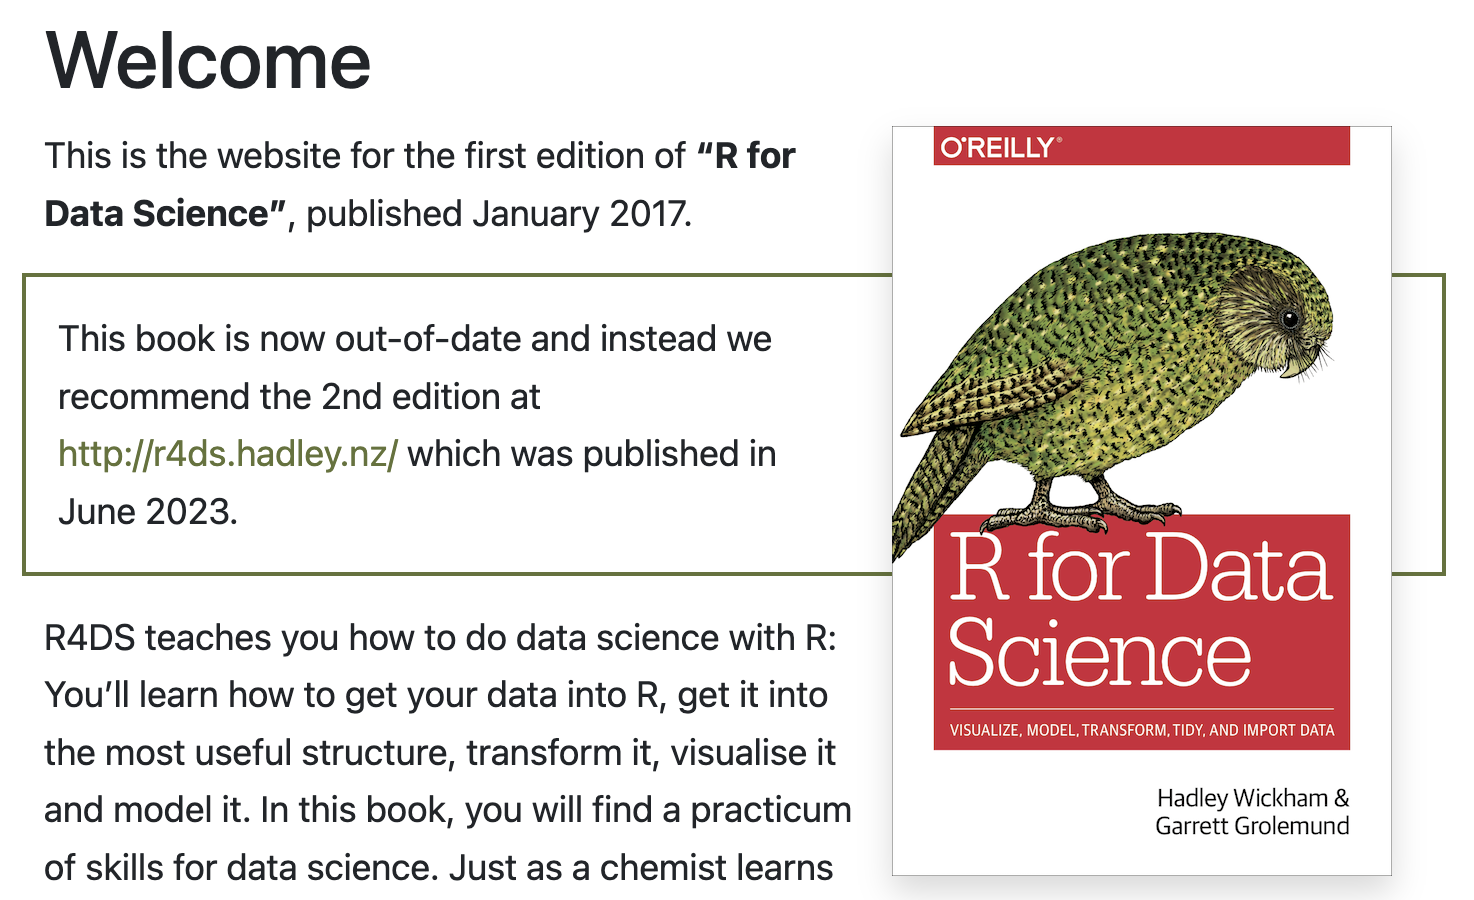
\includegraphics{./img/RforDS.png}

\subsection{Tidyverse basics}\label{tidyverse-basics}

\begin{itemize}
\tightlist
\item
  As it is difficult to change how fundamental base R structures/functions work, the tidyverse suite of packages creates and uses data structures, functions, and operators to make working with data more intuitive.
\item
  The two most basic changes are in the use of pipes and tibbles.
\end{itemize}

\begin{Shaded}
\begin{Highlighting}[]
\CommentTok{\# Packages for tidyverse demo}
\FunctionTok{library}\NormalTok{(datasets)}
\FunctionTok{library}\NormalTok{(tidyverse)}
\end{Highlighting}
\end{Shaded}

\subsection{Pipes}\label{pipes}

\begin{itemize}
\tightlist
\item
  Stringing together commands in R can be quite daunting. Also, trying to understand code that has many nested functions can be confusing.
\item
  To make R code more human readable, the Tidyverse tools use the pipe, \texttt{\%\textgreater{}\%}, which was acquired from the magrittr package and comes installed automatically with Tidyverse.
\item
  The pipe allows the output of a previous command to be used as input to another command instead
  of using nested functions.
\item
  Hint: The shortcut to write pipe is \texttt{shift\ +\ command\ +\ M}.
\end{itemize}

\subsubsection{Exercise: pipes}\label{exercise-pipes}

\begin{itemize}
\tightlist
\item
  Base R method of running more than one command
\end{itemize}

\begin{Shaded}
\begin{Highlighting}[]
\FunctionTok{sqrt}\NormalTok{(}\DecValTok{83}\NormalTok{)}
\FunctionTok{round}\NormalTok{(}\FunctionTok{sqrt}\NormalTok{(}\DecValTok{83}\NormalTok{), }\AttributeTok{digit =} \DecValTok{2}\NormalTok{)}
\end{Highlighting}
\end{Shaded}

\begin{itemize}
\tightlist
\item
  Running more than one command with piping
\end{itemize}

\begin{Shaded}
\begin{Highlighting}[]
\FunctionTok{sqrt}\NormalTok{(}\DecValTok{83}\NormalTok{) }\SpecialCharTok{\%\textgreater{}\%} \FunctionTok{round}\NormalTok{(}\AttributeTok{digit =} \DecValTok{2}\NormalTok{)}
\end{Highlighting}
\end{Shaded}

\subsection{Tibbles}\label{tibbles}

\begin{itemize}
\tightlist
\item
  A core component of the tidyverse is the tibble.
\item
  Tibbles are a modern rework of the standard \texttt{data.frame}, with some internal improvements to make code more reliable.
\item
  They are data frames but do not follow all of the same rules. For example, tibbles can have column names that are not normally allowed, such as numbers/symbols.
\item
  Tibbles can be created directly using the \texttt{tibble()} function or data frames can be converted into tibbles using \texttt{as\_tibble(name\_of\_df)}.
\item
  In this section of code, the iris data frame is converted into a tibble. The iris dataset consists of five variables: \texttt{Sepal.Length}, \texttt{Sepal.Width}, \texttt{Petal.Length}, \texttt{Petal.Width}, and \texttt{Species}.
\end{itemize}

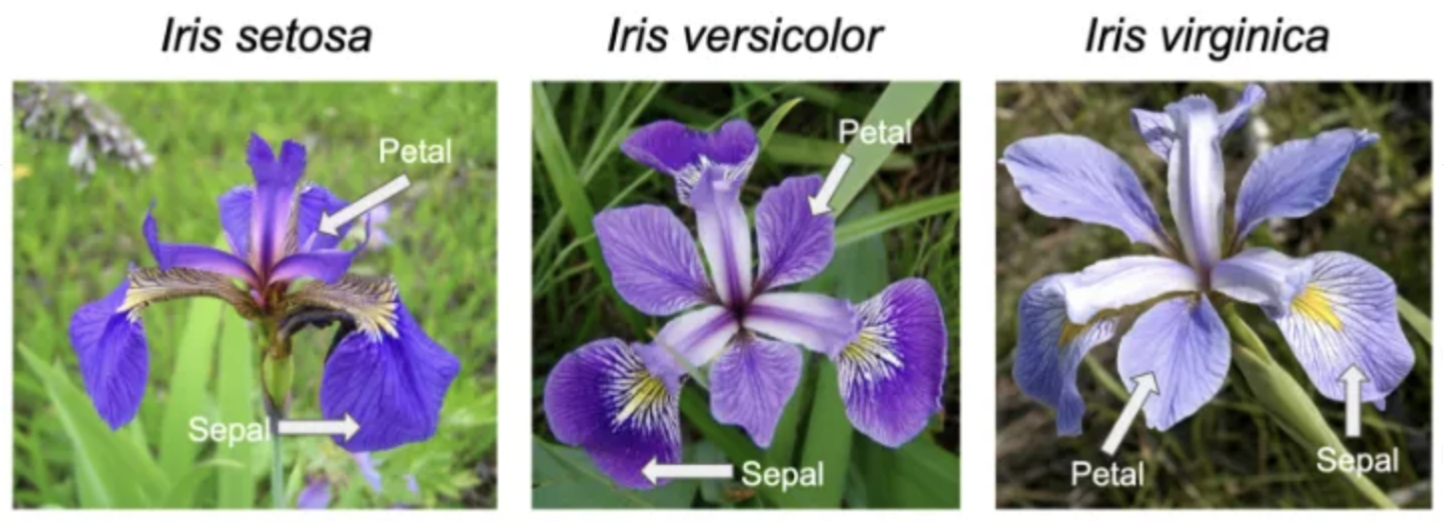
\includegraphics{./img/iris_data.png}

\begin{Shaded}
\begin{Highlighting}[]
\CommentTok{\# Loading the iris dataset from the datasets package}
\FunctionTok{data}\NormalTok{(}\StringTok{"iris"}\NormalTok{)}

\CommentTok{\# Converting the iris data.frame into a tibble object}
\NormalTok{tibble\_iris }\OtherTok{\textless{}{-}} \FunctionTok{as\_tibble}\NormalTok{(iris)}

\CommentTok{\# Using a data.frame as a tibble with a pipe operator}
\NormalTok{iris }\SpecialCharTok{\%\textgreater{}\%} \FunctionTok{as\_tibble}\NormalTok{()}
\end{Highlighting}
\end{Shaded}

\subsection{Differences between tibbles and data.frames}\label{differences-between-tibbles-and-data.frames}

\begin{itemize}
\tightlist
\item
  The main differences between \texttt{tibbles} and \texttt{data.frames} relate to printing and subsetting.
\end{itemize}

\subsubsection{Printing}\label{printing}

\begin{itemize}
\tightlist
\item
  A nice feature of a tibble is that when printing a variable to screen, it will show only the first 10 rows and the columns that fit to the screen by default.
\end{itemize}

\begin{Shaded}
\begin{Highlighting}[]
\CommentTok{\# Default printing of data.frame}
\NormalTok{iris }\CommentTok{\# Prints 150 rows}

\CommentTok{\# Default printing of tibble}
\NormalTok{iris }\SpecialCharTok{\%\textgreater{}\%}
  \FunctionTok{as\_tibble}\NormalTok{() }\CommentTok{\# Prints 10 row}
\end{Highlighting}
\end{Shaded}

\begin{itemize}
\tightlist
\item
  This is nice since you don't have to specify head() to take a quick look at your dataset.
\item
  If it is desirable to view more of the dataset, the print() function can change the number of rows or columns displayed.
\end{itemize}

\begin{Shaded}
\begin{Highlighting}[]
\CommentTok{\# Printing of tibble with print() {-} change defaults}
\NormalTok{iris }\SpecialCharTok{\%\textgreater{}\%}
  \FunctionTok{as\_tibble}\NormalTok{() }\SpecialCharTok{\%\textgreater{}\%}
  \FunctionTok{print}\NormalTok{(}\AttributeTok{n =} \DecValTok{20}\NormalTok{, }\AttributeTok{width =} \ConstantTok{Inf}\NormalTok{)}
\end{Highlighting}
\end{Shaded}

\subsubsection{Subsetting}\label{subsetting}

\begin{itemize}
\tightlist
\item
  When subsetting base R data.frames the default behavior is to simplify the output to the simplest data structure (i.e., a vector).
\item
  If you use piping to subset a data frame, then the notation is slightly different from base R, requiring a placeholder \texttt{.} prior to the \texttt{{[}\ {]}} or \texttt{\$}.
\end{itemize}

\begin{Shaded}
\begin{Highlighting}[]
\CommentTok{\# Subsetting the Species variable in base R}
\NormalTok{iris}\SpecialCharTok{$}\NormalTok{Species}
\NormalTok{iris[ ,}\StringTok{"Species"}\NormalTok{]}

\CommentTok{\# Subsetting the Species variable in output using a pipe}
\NormalTok{iris }\SpecialCharTok{\%\textgreater{}\%}\NormalTok{ .}\SpecialCharTok{$}\NormalTok{Species}
\NormalTok{iris }\SpecialCharTok{\%\textgreater{}\%}\NormalTok{ .[ ,}\StringTok{"Species"}\NormalTok{]}
\end{Highlighting}
\end{Shaded}

\begin{itemize}
\tightlist
\item
  Note that some older functions do not work with tibbles, so if you need to convert a tibble to a data.frame, the function as.data.frame(name\_of\_tibble) will easily convert it.
\end{itemize}

\subsection{Tidyverse tools}\label{tidyverse-tools}

\begin{itemize}
\tightlist
\item
  Tidyverse has many tools for data wrangling, cleaning, and visualization.
\end{itemize}

\subsubsection{dplyr}\label{dplyr}

\begin{itemize}
\item
  Perhaps the most useful tool in the tidyverse is dplyr. It's a Swiss-army knife for data wrangling.
\item
  dplyr has many handy functions:

  \begin{itemize}
  \tightlist
  \item
    \texttt{select()} extracts columns and returns a tibble.
  \item
    \texttt{arrange()} changes the ordering of the rows.
  \item
    \texttt{filter()} picks cases based on their values.
  \item
    \texttt{mutate()} adds new variables that are functions of existing variables.
  \item
    \texttt{rename()} easily changes the name of a column(s).
  \item
    \texttt{summarise()} reduces multiple values down to a single summary.
  \item
    \texttt{pull()} extracts a single column as a vector.
  \item
    \texttt{\_join()} group of functions that merge two data frames together (e.g., \texttt{inner\_join()}, \texttt{left\_join()}, \texttt{right\_join()}, and \texttt{full\_join()}).
  \end{itemize}
\item
  Here is an example of the \texttt{select()}, \texttt{filter()}, and \texttt{summarise()} functions using the iris dataset.
\end{itemize}

\begin{Shaded}
\begin{Highlighting}[]
\CommentTok{\# Only select the columns related to the Sepal of the iris}
\NormalTok{iris }\SpecialCharTok{\%\textgreater{}\%}
  \FunctionTok{select}\NormalTok{(Sepal.Length,Sepal.Width) }\SpecialCharTok{\%\textgreater{}\%}
  \FunctionTok{head}\NormalTok{()}
\end{Highlighting}
\end{Shaded}

\begin{Shaded}
\begin{Highlighting}[]
\CommentTok{\#F ilter for irises with a Sepal.Length greater than 5 and Sepal.Width greater than 4}
\NormalTok{iris }\SpecialCharTok{\%\textgreater{}\%}
  \FunctionTok{filter}\NormalTok{(Sepal.Length }\SpecialCharTok{\textgreater{}} \DecValTok{5}\NormalTok{, Sepal.Width }\SpecialCharTok{\textgreater{}} \DecValTok{4}\NormalTok{)}
\end{Highlighting}
\end{Shaded}

\begin{Shaded}
\begin{Highlighting}[]
\CommentTok{\# Calculate the average Sepal.Length and Sepal.Width for each iris Species}
\NormalTok{iris }\SpecialCharTok{\%\textgreater{}\%}
  \FunctionTok{group\_by}\NormalTok{(Species) }\SpecialCharTok{\%\textgreater{}\%}
  \FunctionTok{summarise}\NormalTok{(}\AttributeTok{mean.Sepal.Length =} \FunctionTok{mean}\NormalTok{(Sepal.Length), }\AttributeTok{mean.Sepal.width =} \FunctionTok{mean}\NormalTok{(Sepal.Width))}
\end{Highlighting}
\end{Shaded}

\section{Final exercise}\label{final-exercise-1}

\begin{enumerate}
\def\labelenumi{\arabic{enumi}.}
\tightlist
\item
  Subset the \texttt{Species} column from the iris dataset using a pipe.
\end{enumerate}

\begin{itemize}
\tightlist
\item
  Hint: Use a \texttt{.} before the \texttt{{[}\ {]}} or \texttt{\$}.
\end{itemize}

\begin{enumerate}
\def\labelenumi{\arabic{enumi}.}
\setcounter{enumi}{1}
\tightlist
\item
  Select the \texttt{Petal.Length} and \texttt{Petal.Width} columns from the iris dataset.
\item
  Find the average \texttt{Petal.Length} and \texttt{Petal.Width} for each iris Species.
\end{enumerate}

\section{Bonus: R Markdown}\label{bonus-r-markdown}

\begin{itemize}
\tightlist
\item
  If you have not downloaded the R Markdown yet, please go to \url{https://rmarkdown.rstudio.com/lesson-1.html} and download the \texttt{rmarkdown} package.
\item
  R Markdown is a tool for reproducible documentation in statistics. R markdown generates a new file that contains selected text, code, and results from the \texttt{.Rmd} file.
\item
  The newly created file can be a finished website, PDF document, Word document, slide (beamer, powerpoint, xaringan) show, notebook, handout, book, dashboard, Shiny Apps, package vignette, or more.
\end{itemize}

\subsection{How does the R Markdown work?}\label{how-does-the-r-markdown-work}


\includegraphics{./img/rmarkdown_works.png}

\begin{itemize}
\tightlist
\item
  According to \url{https://rmarkdown.rstudio.com/lesson-2.html},

  \begin{itemize}
  \tightlist
  \item
    When you run render, R Markdown feeds the \texttt{.Rmd} file to \texttt{knitr}, which executes all of the code chunks and creates a new markdown (.md) document which includes the code and its output.
  \item
    The markdown file generated by \texttt{knitr} is then processed by \texttt{pandoc} which is responsible for creating the finished format.
  \item
    This may sound complicated, but R Markdown makes it extremely simple by encapsulating all of the above processing into a single render function.
  \end{itemize}
\end{itemize}

\subsubsection{Practice}\label{practice}

\begin{itemize}
\tightlist
\item
  Generate any PDF document from R Markdown by knitting your markdown file.
\item
  You may need to visit:

  \begin{itemize}
  \tightlist
  \item
    \url{https://yihui.org/tinytex/}
  \item
    \url{https://yihui.org/tinytex/r/\#debugging}
  \end{itemize}
\end{itemize}

\chapter{Summarizing Data}\label{summarizing-data}

\section{Are you ready?}\label{are-you-ready}

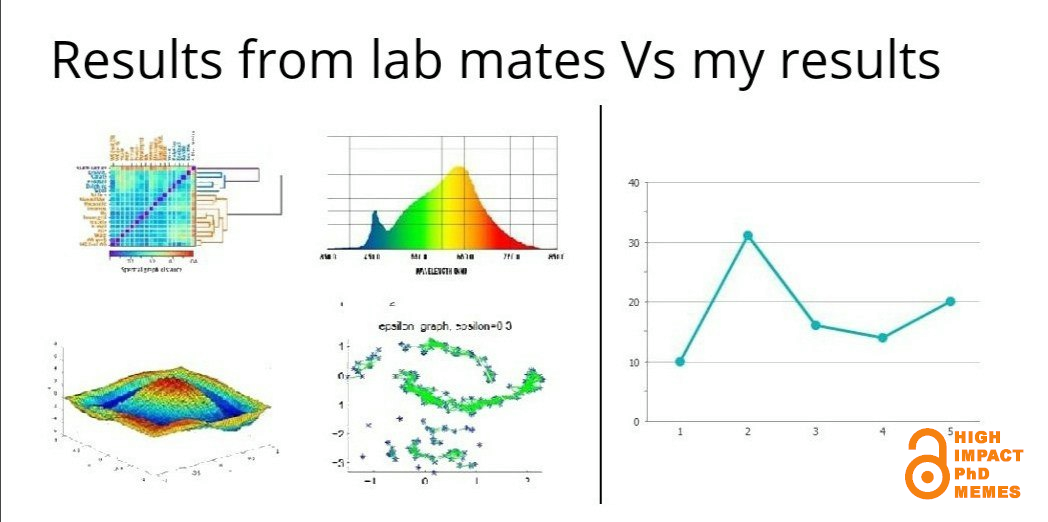
\includegraphics{./img/fun_datvis_meme.png}

\subsection{Wait\ldots{} you guys are getting results???!}\label{wait-you-guys-are-getting-results}


\includegraphics{./img/wait_results.jpg}

\section{Packages}\label{packages-1}

\begin{itemize}
\tightlist
\item
  Here is a list of packages that we will use today:

  \begin{itemize}
  \tightlist
  \item
    \texttt{modeest} has the \texttt{mfv()} function for the mode.
  \item
    \texttt{moments} has the \texttt{skewness()} and \texttt{kurtosis()} functions.
  \item
    \texttt{tidyverse} contains the \texttt{ggplot2} package for data visualization.
  \end{itemize}
\item
  For those who hope to dive into the fancier data visualization tools, consider:

  \begin{itemize}
  \tightlist
  \item
    RShiny at \url{https://shiny.posit.co/r/gallery/}.
  \item
    Extensions of the \texttt{ggplot2} package at \url{https://exts.ggplot2.tidyverse.org/gallery/}.
  \end{itemize}
\end{itemize}

\section{Numerical methods}\label{numerical-methods}

\subsection{Peabody data}\label{peabody-data}

\begin{itemize}
\item
  For the purpose of today's demonstration, we will use the following data from 40 children who completed the Peabody Developmental Motor Scales (PDMS).
\item
  The PDMS is a popular standardized test used by physical and occupational therapists for children less than six.
\item
  The variables include peabody scores, gender, and age (in months).
\item
  The dataset is as follows:
\end{itemize}

\begin{Shaded}
\begin{Highlighting}[]
\CommentTok{\# Peabody data}
\NormalTok{peabody }\OtherTok{\textless{}{-}} \FunctionTok{c}\NormalTok{(}\DecValTok{123}\NormalTok{,}\DecValTok{99}\NormalTok{,}\DecValTok{80}\NormalTok{,}\DecValTok{81}\NormalTok{,}\DecValTok{90}\NormalTok{,}\DecValTok{104}\NormalTok{,}\DecValTok{69}\NormalTok{,}\DecValTok{86}\NormalTok{,}\DecValTok{107}\NormalTok{,}\DecValTok{94}\NormalTok{,}\DecValTok{82}\NormalTok{,}\DecValTok{99}\NormalTok{,}\DecValTok{83}\NormalTok{,}\DecValTok{98}\NormalTok{,}\DecValTok{86}\NormalTok{,}\DecValTok{74}\NormalTok{,}\DecValTok{67}\NormalTok{,}\DecValTok{90}\NormalTok{,}\DecValTok{106}\NormalTok{,}\DecValTok{102}\NormalTok{,}
             \DecValTok{68}\NormalTok{,}\DecValTok{80}\NormalTok{,}\DecValTok{76}\NormalTok{,}\DecValTok{65}\NormalTok{,}\DecValTok{69}\NormalTok{,}\DecValTok{81}\NormalTok{,}\DecValTok{76}\NormalTok{,}\DecValTok{68}\NormalTok{,}\DecValTok{84}\NormalTok{,}\DecValTok{88}\NormalTok{,}\DecValTok{68}\NormalTok{,}\DecValTok{92}\NormalTok{,}\DecValTok{92}\NormalTok{,}\DecValTok{97}\NormalTok{,}\DecValTok{78}\NormalTok{,}\DecValTok{77}\NormalTok{,}\DecValTok{94}\NormalTok{,}\DecValTok{74}\NormalTok{,}\DecValTok{89}\NormalTok{,}\DecValTok{68}\NormalTok{)}

\NormalTok{gender }\OtherTok{\textless{}{-}} \FunctionTok{c}\NormalTok{(}\StringTok{"M"}\NormalTok{,}\StringTok{"F"}\NormalTok{,}\StringTok{"F"}\NormalTok{,}\StringTok{"F"}\NormalTok{,}\StringTok{"F"}\NormalTok{,}\StringTok{"M"}\NormalTok{,}\StringTok{"F"}\NormalTok{,}\StringTok{"F"}\NormalTok{,}\StringTok{"F"}\NormalTok{,}\StringTok{"F"}\NormalTok{,}\StringTok{"M"}\NormalTok{,}\StringTok{"M"}\NormalTok{,}\StringTok{"M"}\NormalTok{,}\StringTok{"M"}\NormalTok{,}\StringTok{"M"}\NormalTok{,}\StringTok{"M"}\NormalTok{,}\StringTok{"M"}\NormalTok{,}
            \StringTok{"M"}\NormalTok{,}\StringTok{"M"}\NormalTok{,}\StringTok{"M"}\NormalTok{,}\StringTok{"F"}\NormalTok{,}\StringTok{"F"}\NormalTok{,}\StringTok{"F"}\NormalTok{,}\StringTok{"M"}\NormalTok{,}\StringTok{"F"}\NormalTok{,}\StringTok{"F"}\NormalTok{,}\StringTok{"F"}\NormalTok{,}\StringTok{"M"}\NormalTok{,}\StringTok{"M"}\NormalTok{,}\StringTok{"F"}\NormalTok{,}\StringTok{"M"}\NormalTok{,}\StringTok{"M"}\NormalTok{,}\StringTok{"M"}\NormalTok{,}\StringTok{"M"}\NormalTok{,}
            \StringTok{"M"}\NormalTok{,}\StringTok{"M"}\NormalTok{,}\StringTok{"M"}\NormalTok{,}\StringTok{"M"}\NormalTok{,}\StringTok{"M"}\NormalTok{,}\StringTok{"M"}\NormalTok{)}

\NormalTok{age }\OtherTok{\textless{}{-}} \FunctionTok{c}\NormalTok{(}\DecValTok{35}\NormalTok{,}\DecValTok{45}\NormalTok{,}\DecValTok{38}\NormalTok{,}\DecValTok{40}\NormalTok{,}\DecValTok{38}\NormalTok{,}\DecValTok{42}\NormalTok{,}\DecValTok{36}\NormalTok{,}\DecValTok{45}\NormalTok{,}\DecValTok{34}\NormalTok{,}\DecValTok{36}\NormalTok{,}\DecValTok{36}\NormalTok{,}\DecValTok{51}\NormalTok{,}\DecValTok{34}\NormalTok{,}\DecValTok{35}\NormalTok{,}\DecValTok{37}\NormalTok{,}\DecValTok{37}\NormalTok{,}\DecValTok{36}\NormalTok{,}\DecValTok{36}\NormalTok{,}\DecValTok{37}\NormalTok{,}\DecValTok{32}\NormalTok{,}\DecValTok{22}\NormalTok{,}\DecValTok{28}\NormalTok{,}\DecValTok{18}\NormalTok{,}\DecValTok{20}\NormalTok{,}
         \DecValTok{25}\NormalTok{,}\DecValTok{18}\NormalTok{,}\DecValTok{14}\NormalTok{,}\DecValTok{26}\NormalTok{,}\DecValTok{14}\NormalTok{,}\DecValTok{24}\NormalTok{,}\DecValTok{14}\NormalTok{,}\DecValTok{26}\NormalTok{,}\DecValTok{11}\NormalTok{,}\DecValTok{12}\NormalTok{,}\DecValTok{26}\NormalTok{,}\DecValTok{17}\NormalTok{,}\DecValTok{16}\NormalTok{,}\DecValTok{23}\NormalTok{,}\DecValTok{12}\NormalTok{,}\DecValTok{13}\NormalTok{)}
\end{Highlighting}
\end{Shaded}

\begin{itemize}
\tightlist
\item
  These variables can be stored in a data frame with the following code:
\end{itemize}

\begin{Shaded}
\begin{Highlighting}[]
\CommentTok{\# Make a data frame}
\NormalTok{peabody\_df }\OtherTok{\textless{}{-}} \FunctionTok{data.frame}\NormalTok{(}\AttributeTok{peabody =}\NormalTok{ peabody, }\AttributeTok{gender =}\NormalTok{ gender, }\AttributeTok{age =}\NormalTok{ age)}
\end{Highlighting}
\end{Shaded}

\subsection{Central tendency}\label{central-tendency}

\begin{itemize}
\tightlist
\item
  Mean
\end{itemize}

\begin{Shaded}
\begin{Highlighting}[]
\FunctionTok{mean}\NormalTok{(peabody)}
\end{Highlighting}
\end{Shaded}

\begin{verbatim}
## [1] 85.1
\end{verbatim}

\begin{Shaded}
\begin{Highlighting}[]
\FunctionTok{mean}\NormalTok{(peabody\_df}\SpecialCharTok{$}\NormalTok{peabody)}
\end{Highlighting}
\end{Shaded}

\begin{verbatim}
## [1] 85.1
\end{verbatim}

\begin{itemize}
\tightlist
\item
  Median
\end{itemize}

\begin{Shaded}
\begin{Highlighting}[]
\FunctionTok{median}\NormalTok{(peabody)}
\end{Highlighting}
\end{Shaded}

\begin{verbatim}
## [1] 83.5
\end{verbatim}

\begin{Shaded}
\begin{Highlighting}[]
\FunctionTok{median}\NormalTok{(peabody\_df}\SpecialCharTok{$}\NormalTok{peabody)}
\end{Highlighting}
\end{Shaded}

\begin{verbatim}
## [1] 83.5
\end{verbatim}

\begin{itemize}
\tightlist
\item
  Mode
\end{itemize}

\begin{Shaded}
\begin{Highlighting}[]
\FunctionTok{library}\NormalTok{(modeest)}
\FunctionTok{mfv}\NormalTok{(peabody)}
\end{Highlighting}
\end{Shaded}

\begin{verbatim}
## [1] 68
\end{verbatim}

\subsection{Variability}\label{variability}

\begin{itemize}
\tightlist
\item
  Variance
\end{itemize}

\begin{Shaded}
\begin{Highlighting}[]
\FunctionTok{var}\NormalTok{(peabody)}
\end{Highlighting}
\end{Shaded}

\begin{verbatim}
## [1] 181.1692
\end{verbatim}

\begin{itemize}
\tightlist
\item
  Standard deviation
\end{itemize}

\begin{Shaded}
\begin{Highlighting}[]
\FunctionTok{sd}\NormalTok{(peabody)}
\end{Highlighting}
\end{Shaded}

\begin{verbatim}
## [1] 13.45991
\end{verbatim}

\subsection{Skewness}\label{skewness}

\begin{itemize}
\item
  There are multiple methods that can be used to calculate skewness in R:
\item
  You could use the formula for skewness.
\end{itemize}

\begin{Shaded}
\begin{Highlighting}[]
\CommentTok{\# Define sample size}
\NormalTok{n }\OtherTok{\textless{}{-}} \FunctionTok{length}\NormalTok{(peabody)}

\CommentTok{\# Compute the skewness}
\NormalTok{(}\FunctionTok{sum}\NormalTok{((peabody}\SpecialCharTok{{-}}\FunctionTok{mean}\NormalTok{(peabody))}\SpecialCharTok{\^{}}\DecValTok{3}\NormalTok{)}\SpecialCharTok{/}\NormalTok{n)}\SpecialCharTok{/}\NormalTok{(}\FunctionTok{sum}\NormalTok{((peabody}\SpecialCharTok{{-}}\FunctionTok{mean}\NormalTok{(peabody))}\SpecialCharTok{\^{}}\DecValTok{2}\NormalTok{)}\SpecialCharTok{/}\NormalTok{n)}\SpecialCharTok{\^{}}\NormalTok{(}\DecValTok{3}\SpecialCharTok{/}\DecValTok{2}\NormalTok{)}
\end{Highlighting}
\end{Shaded}

\begin{verbatim}
## [1] 0.524655
\end{verbatim}

\begin{itemize}
\tightlist
\item
  But the \texttt{skewness()} function in the \texttt{moments} package makes it even easier.
\end{itemize}

\begin{Shaded}
\begin{Highlighting}[]
\FunctionTok{library}\NormalTok{(moments)}
\end{Highlighting}
\end{Shaded}

\begin{verbatim}
## 
## Attaching package: 'moments'
\end{verbatim}

\begin{verbatim}
## The following object is masked from 'package:modeest':
## 
##     skewness
\end{verbatim}

\begin{Shaded}
\begin{Highlighting}[]
\FunctionTok{skewness}\NormalTok{(peabody)}
\end{Highlighting}
\end{Shaded}

\begin{verbatim}
## [1] 0.524655
\end{verbatim}

\subsection{Kurtosis}\label{kurtosis}

\begin{itemize}
\item
  There are multiple methods for calculating kurtosis in R.
\item
  You can use the formula:
\end{itemize}

\begin{Shaded}
\begin{Highlighting}[]
\NormalTok{n }\OtherTok{\textless{}{-}} \FunctionTok{length}\NormalTok{(peabody)}
\NormalTok{(}\FunctionTok{sum}\NormalTok{((peabody}\SpecialCharTok{{-}}\FunctionTok{mean}\NormalTok{(peabody))}\SpecialCharTok{\^{}}\DecValTok{4}\NormalTok{)}\SpecialCharTok{/}\NormalTok{n)}\SpecialCharTok{/}\NormalTok{(}\FunctionTok{sum}\NormalTok{((peabody}\SpecialCharTok{{-}}\FunctionTok{mean}\NormalTok{(peabody))}\SpecialCharTok{\^{}}\DecValTok{2}\NormalTok{)}\SpecialCharTok{/}\NormalTok{n)}\SpecialCharTok{\^{}}\DecValTok{2}
\end{Highlighting}
\end{Shaded}

\begin{verbatim}
## [1] 2.911796
\end{verbatim}

\begin{itemize}
\tightlist
\item
  Or you can use the \texttt{kurtosis()} function in the \texttt{moments} package.
\end{itemize}

\begin{Shaded}
\begin{Highlighting}[]
\FunctionTok{kurtosis}\NormalTok{(peabody)}
\end{Highlighting}
\end{Shaded}

\begin{verbatim}
## [1] 2.911796
\end{verbatim}

\subsection{Using the tidyverse package}\label{using-the-tidyverse-package}

\begin{itemize}
\tightlist
\item
  tidyverse allows us to use the \texttt{summarise()} function.

  \begin{itemize}
  \tightlist
  \item
    which allows us to get various descriptive statistics such as minimum, maximum, mean, median, variance, standard deviation, skewness, kurtosis, etc.
  \end{itemize}
\item
  As a small exercise, try to run the code below. What do you see?
\end{itemize}

\begin{Shaded}
\begin{Highlighting}[]
\FunctionTok{summarise}\NormalTok{(peabody\_df,}
          \AttributeTok{mean.peabody =} \FunctionTok{mean}\NormalTok{(peabody),}
          \AttributeTok{sd.peabody =} \FunctionTok{sd}\NormalTok{(peabody),}
          \AttributeTok{skew.peabody =}\NormalTok{ moments}\SpecialCharTok{::}\FunctionTok{skewness}\NormalTok{(peabody),}
          \AttributeTok{kurt.peabody =}\NormalTok{ moments}\SpecialCharTok{::}\FunctionTok{kurtosis}\NormalTok{(peabody))}
\end{Highlighting}
\end{Shaded}

\section{Visual methods}\label{visual-methods}

\begin{itemize}
\item
  Be sure to refer to the cheatsheet I have attached on CatCourses!
\item
  Every useful piece of information is there!
\end{itemize}

\subsection{Using the tidyverse package}\label{using-the-tidyverse-package-1}

\begin{itemize}
\item
  The \texttt{ggplot2} package is a core component of the tidyverse that allows us to build data visualizations.
\item
  ChatGPT is so good at programming \texttt{ggplot2} code for you. But of course, sometimes it itself does produce wrong code, particularly when you want to do complicated visualizations.

  \begin{itemize}
  \tightlist
  \item
    It is suggested to know the fundamental grammar to be a smart user of the AI!
  \end{itemize}
\item
  The idea behind \texttt{ggplot2} is that every new concept we introduce will be layered on top of the information we've already learned.
\item
  In this way, \texttt{ggplot2} uses layers of information added on top of each other to help build the graph.

  \begin{itemize}
  \tightlist
  \item
    This is most evidenced by how each line is separated by a plus sign (+). Each line of code is a different layer of the graph.
  \end{itemize}
\item
  You'll see what I mean as we go through several example graphs.
\item
  Remember to work with a tibble instead of a data frame. Tibbles work much better in tidyverse.
\end{itemize}

\begin{Shaded}
\begin{Highlighting}[]
\FunctionTok{library}\NormalTok{(tidyverse)}
\end{Highlighting}
\end{Shaded}

\begin{verbatim}
## Warning: package 'ggplot2' was built under R version 4.2.3
\end{verbatim}

\begin{verbatim}
## Warning: package 'tidyr' was built under R version 4.2.3
\end{verbatim}

\begin{verbatim}
## Warning: package 'readr' was built under R version 4.2.3
\end{verbatim}

\begin{verbatim}
## Warning: package 'dplyr' was built under R version 4.2.3
\end{verbatim}

\begin{verbatim}
## Warning: package 'stringr' was built under R version 4.2.3
\end{verbatim}

\begin{verbatim}
## -- Attaching core tidyverse packages ------------------------ tidyverse 2.0.0 --
## v dplyr     1.1.4     v readr     2.1.5
## v forcats   1.0.0     v stringr   1.5.1
## v ggplot2   3.5.1     v tibble    3.2.1
## v lubridate 1.9.3     v tidyr     1.3.1
## v purrr     1.0.2     
## -- Conflicts ------------------------------------------ tidyverse_conflicts() --
## x dplyr::filter() masks stats::filter()
## x dplyr::lag()    masks stats::lag()
## i Use the conflicted package (<http://conflicted.r-lib.org/>) to force all conflicts to become errors
\end{verbatim}

\begin{Shaded}
\begin{Highlighting}[]
\NormalTok{peabody\_tib }\OtherTok{\textless{}{-}} \FunctionTok{as\_tibble}\NormalTok{(peabody\_df)}
\NormalTok{peabody\_tib}
\end{Highlighting}
\end{Shaded}

\begin{verbatim}
## # A tibble: 40 x 3
##    peabody gender   age
##      <dbl> <chr>  <dbl>
##  1     123 M         35
##  2      99 F         45
##  3      80 F         38
##  4      81 F         40
##  5      90 F         38
##  6     104 M         42
##  7      69 F         36
##  8      86 F         45
##  9     107 F         34
## 10      94 F         36
## # i 30 more rows
\end{verbatim}

\begin{itemize}
\tightlist
\item
  The type of plot you want to make is referred to as a \texttt{geom}. There are dozens of \texttt{geom} options available in \texttt{ggplot2}. For todays' lesson, we will focus on four specific \texttt{geoms}:

  \begin{itemize}
  \tightlist
  \item
    \texttt{geom\_boxplot()}
  \item
    \texttt{geom\_histogram()}
  \item
    \texttt{geom\_bar()}
  \item
    \texttt{geom\_point()}
  \end{itemize}
\item
  When using \texttt{ggplot2}, plots will take the following general form:
\end{itemize}

\begin{Shaded}
\begin{Highlighting}[]
\FunctionTok{ggplot}\NormalTok{(}\AttributeTok{data =}\NormalTok{ DATASET, }\FunctionTok{aes}\NormalTok{(}\FunctionTok{VARIABLE}\NormalTok{(S))) }\SpecialCharTok{+}
  \FunctionTok{geom\_PLOT\_TYPE}\NormalTok{()}
\end{Highlighting}
\end{Shaded}

\begin{itemize}
\item
  First, you start with the \texttt{ggplot()} function, where you will specify the data.
\item
  Second, you will include the \texttt{aes} argument, which is where you specify the variable(s) you want to plot.
\item
  Third, you select the geom type (e.g., \texttt{geom\_boxplot()}) you are interested in plotting. This is also where you can begin to customize your plots.
\end{itemize}

\subsection{Boxplot}\label{boxplot}

\begin{itemize}
\item
  Boxplots are a useful method for presenting the dispersion of the data, the symmetry of the distribution, and the potential outliers (or extreme scores).
\item
  The following code provides a basic \texttt{ggplot2} setup for a boxplot of the peabody scorees:
\end{itemize}

\begin{Shaded}
\begin{Highlighting}[]
\FunctionTok{ggplot}\NormalTok{(}\AttributeTok{data=}\NormalTok{peabody\_tib, }\FunctionTok{aes}\NormalTok{(peabody)) }\SpecialCharTok{+}
  \FunctionTok{geom\_boxplot}\NormalTok{()}
\end{Highlighting}
\end{Shaded}

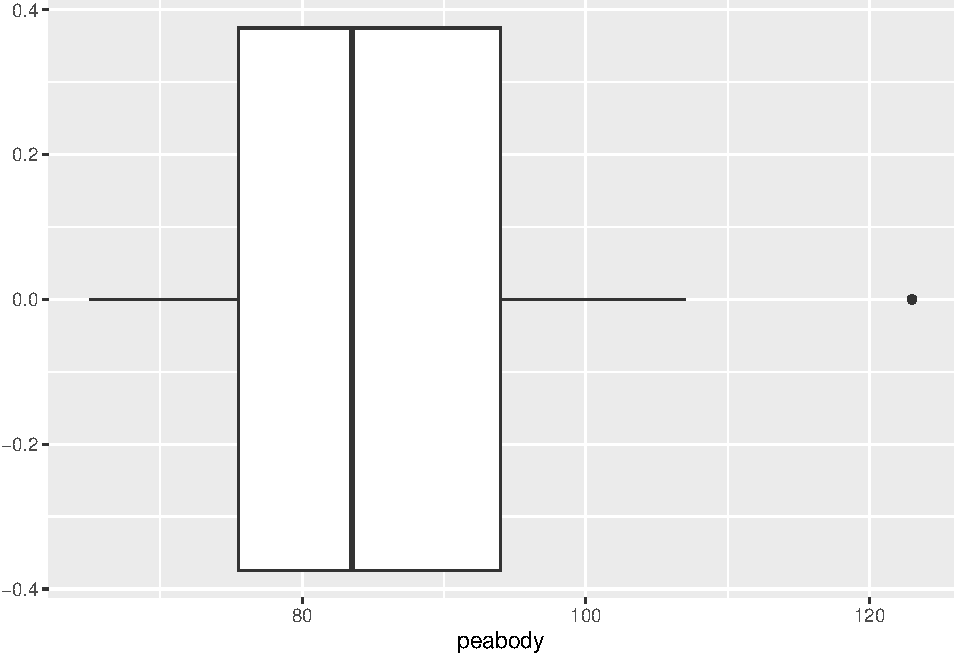
\includegraphics{PSY202A-Modeling-I.Heo_files/figure-latex/unnamed-chunk-72-1.pdf}

\begin{itemize}
\tightlist
\item
  By adding another layer, you can further customize your plot. In the code below, I illustrate how you can change the coloring of the boxplot and remove the tick marks on the x-axis.
\end{itemize}

\begin{Shaded}
\begin{Highlighting}[]
\FunctionTok{ggplot}\NormalTok{(}\AttributeTok{data =}\NormalTok{ peabody\_tib, }\FunctionTok{aes}\NormalTok{(}\AttributeTok{y=}\NormalTok{peabody)) }\SpecialCharTok{+}
  \FunctionTok{geom\_boxplot}\NormalTok{(}\AttributeTok{fill =} \StringTok{"purple"}\NormalTok{, }\AttributeTok{colour =} \StringTok{"black"}\NormalTok{) }\SpecialCharTok{+}
  \FunctionTok{scale\_x\_discrete}\NormalTok{( ) }\DocumentationTok{\#\# removes x{-}axis ticks}
\end{Highlighting}
\end{Shaded}

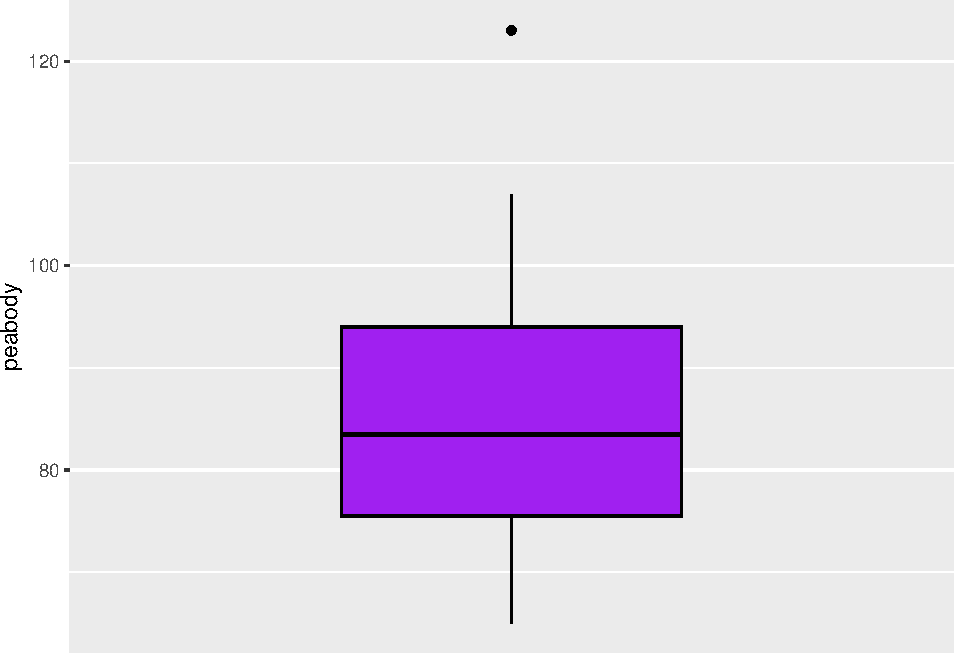
\includegraphics{PSY202A-Modeling-I.Heo_files/figure-latex/unnamed-chunk-73-1.pdf}

\begin{itemize}
\item
  You can also change the shape and color of the outlier.
\item
  All you have to do is add another line of code that specifies the outlier color, shape, and size.
\end{itemize}

\begin{Shaded}
\begin{Highlighting}[]
\FunctionTok{ggplot}\NormalTok{(}\AttributeTok{data =}\NormalTok{ peabody\_tib, }\FunctionTok{aes}\NormalTok{(}\AttributeTok{y=}\NormalTok{peabody)) }\SpecialCharTok{+}
  \FunctionTok{geom\_boxplot}\NormalTok{(}\AttributeTok{fill =} \StringTok{"purple"}\NormalTok{, }\AttributeTok{color =} \StringTok{"black"}\NormalTok{,}
               \AttributeTok{outlier.color =} \StringTok{"red"}\NormalTok{, }\AttributeTok{outlier.shape =} \DecValTok{18}\NormalTok{, }\AttributeTok{outlier.size =} \DecValTok{3}\NormalTok{) }\SpecialCharTok{+}
  \FunctionTok{scale\_x\_discrete}\NormalTok{( ) }\DocumentationTok{\#\# removes x{-}axis ticks}
\end{Highlighting}
\end{Shaded}

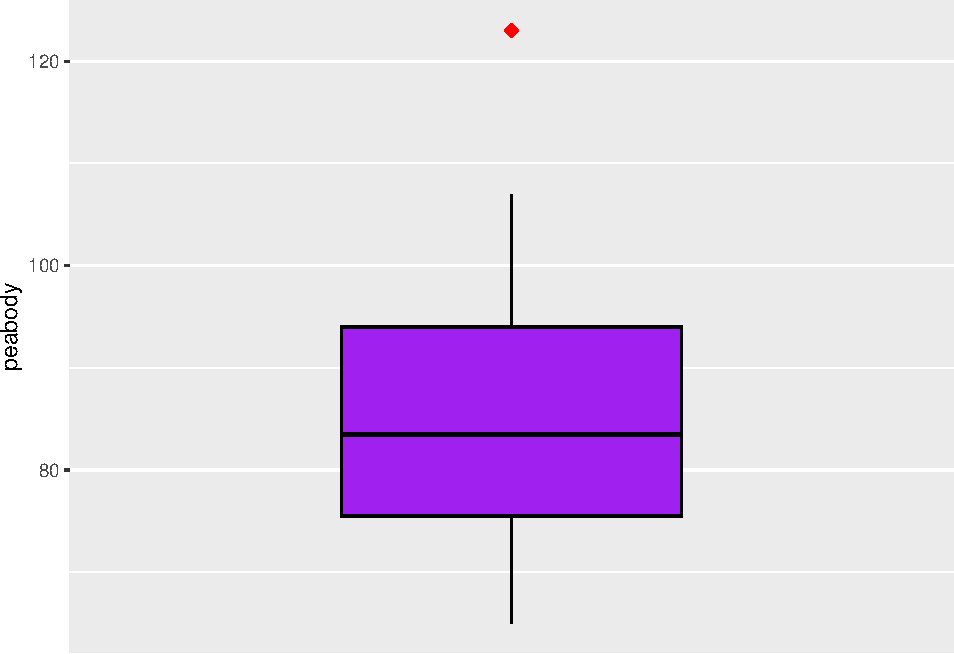
\includegraphics{PSY202A-Modeling-I.Heo_files/figure-latex/unnamed-chunk-74-1.pdf}

\begin{itemize}
\tightlist
\item
  There are several available shapes in \texttt{ggplot2}.

  \begin{itemize}
  \tightlist
  \item
    I provide some examples below, but you can see more here: \url{https://ggplot2.tidyverse.org/articles/ggplot2-specs.html}
  \end{itemize}
\end{itemize}

\begin{Shaded}
\begin{Highlighting}[]
\NormalTok{shapes }\OtherTok{\textless{}{-}} \FunctionTok{data.frame}\NormalTok{(}
  \AttributeTok{shape =} \FunctionTok{c}\NormalTok{(}\DecValTok{0}\SpecialCharTok{:}\DecValTok{19}\NormalTok{, }\DecValTok{22}\NormalTok{, }\DecValTok{21}\NormalTok{, }\DecValTok{24}\NormalTok{, }\DecValTok{23}\NormalTok{, }\DecValTok{20}\NormalTok{),}
  \AttributeTok{x =} \DecValTok{0}\SpecialCharTok{:}\DecValTok{24} \SpecialCharTok{\%/\%} \DecValTok{5}\NormalTok{,}
  \AttributeTok{y =} \SpecialCharTok{{-}}\NormalTok{(}\DecValTok{0}\SpecialCharTok{:}\DecValTok{24} \SpecialCharTok{\%\%} \DecValTok{5}\NormalTok{)}
\NormalTok{)}

\FunctionTok{ggplot}\NormalTok{(shapes, }\FunctionTok{aes}\NormalTok{(x, y)) }\SpecialCharTok{+} 
  \FunctionTok{geom\_point}\NormalTok{(}\FunctionTok{aes}\NormalTok{(}\AttributeTok{shape =}\NormalTok{ shape), }\AttributeTok{size =} \DecValTok{5}\NormalTok{, }\AttributeTok{fill =} \StringTok{"red"}\NormalTok{) }\SpecialCharTok{+}
  \FunctionTok{geom\_text}\NormalTok{(}\FunctionTok{aes}\NormalTok{(}\AttributeTok{label =}\NormalTok{ shape), }\AttributeTok{hjust =} \DecValTok{0}\NormalTok{, }\AttributeTok{nudge\_x =} \FloatTok{0.15}\NormalTok{) }\SpecialCharTok{+}
  \FunctionTok{scale\_shape\_identity}\NormalTok{() }\SpecialCharTok{+}
  \FunctionTok{expand\_limits}\NormalTok{(}\AttributeTok{x =} \FloatTok{4.1}\NormalTok{) }\SpecialCharTok{+}
  \FunctionTok{theme\_void}\NormalTok{()}
\end{Highlighting}
\end{Shaded}

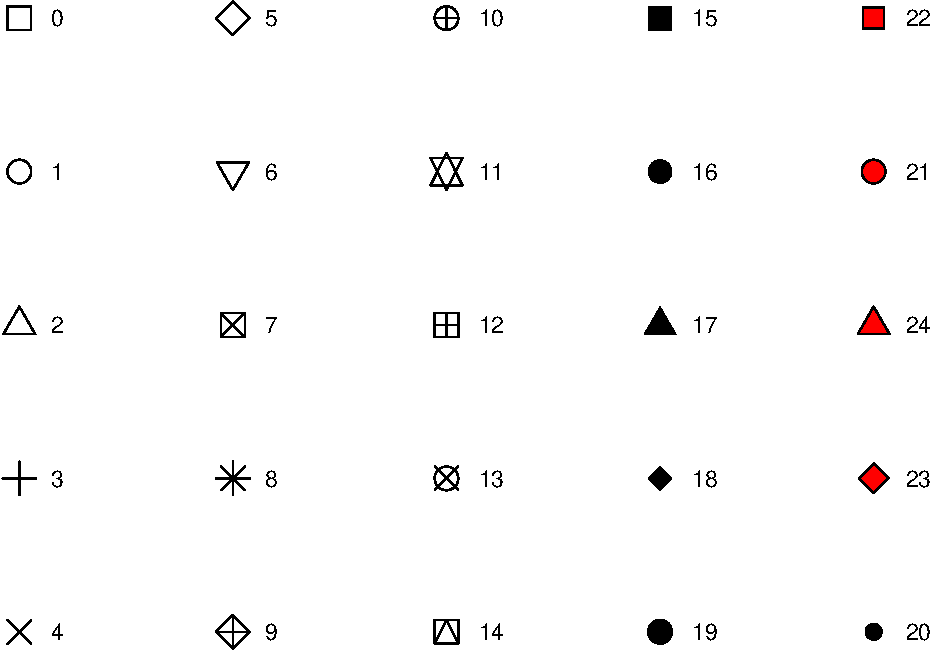
\includegraphics{PSY202A-Modeling-I.Heo_files/figure-latex/unnamed-chunk-75-1.pdf}

\subsection{Histograms}\label{histograms}

\begin{itemize}
\item
  Histograms are a useful method for presenting the dispersion of the data and the symmetry of the distribution.
\item
  The following code provides the setup for a histogram of the peabody scores:
\end{itemize}

\begin{Shaded}
\begin{Highlighting}[]
\FunctionTok{ggplot}\NormalTok{(}\AttributeTok{data =}\NormalTok{ peabody\_tib, }\FunctionTok{aes}\NormalTok{(peabody)) }\SpecialCharTok{+}
  \FunctionTok{geom\_histogram}\NormalTok{(}\AttributeTok{color =} \StringTok{"black"}\NormalTok{, }\AttributeTok{fill =} \StringTok{"green"}\NormalTok{)}
\end{Highlighting}
\end{Shaded}

\begin{verbatim}
## `stat_bin()` using `bins = 30`. Pick better value with `binwidth`.
\end{verbatim}

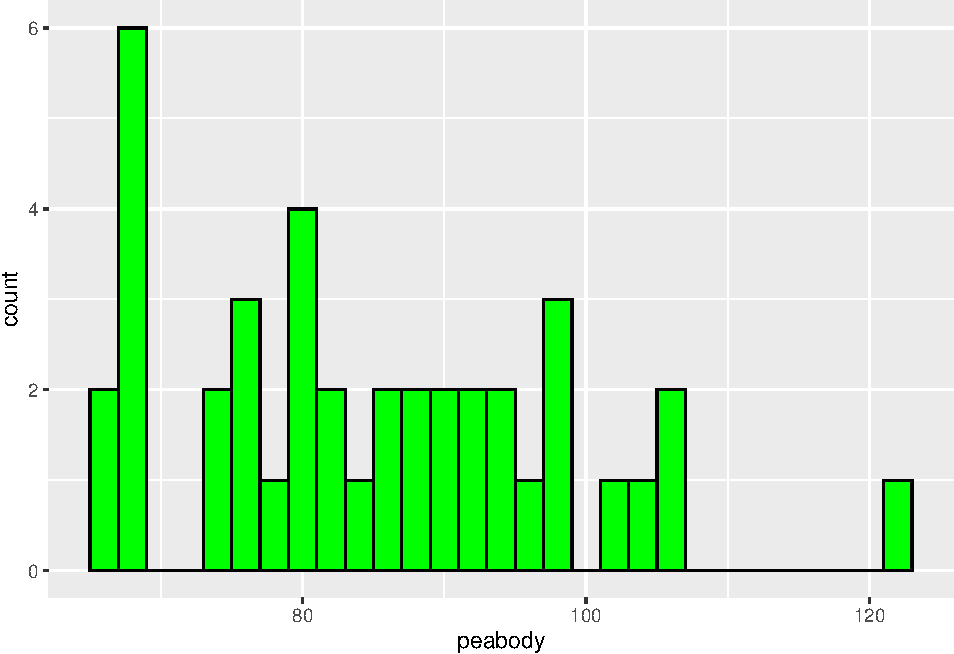
\includegraphics{PSY202A-Modeling-I.Heo_files/figure-latex/unnamed-chunk-76-1.pdf}

\begin{itemize}
\tightlist
\item
  You can change the bindwidth of the histogram using the following code:
\end{itemize}

\begin{Shaded}
\begin{Highlighting}[]
\FunctionTok{ggplot}\NormalTok{(}\AttributeTok{data =}\NormalTok{ peabody\_tib, }\FunctionTok{aes}\NormalTok{(peabody)) }\SpecialCharTok{+}
  \FunctionTok{geom\_histogram}\NormalTok{(}\AttributeTok{color =} \StringTok{"black"}\NormalTok{, }\AttributeTok{fill =} \StringTok{"green"}\NormalTok{,}
               \AttributeTok{binwidth =} \DecValTok{5}\NormalTok{)}
\end{Highlighting}
\end{Shaded}

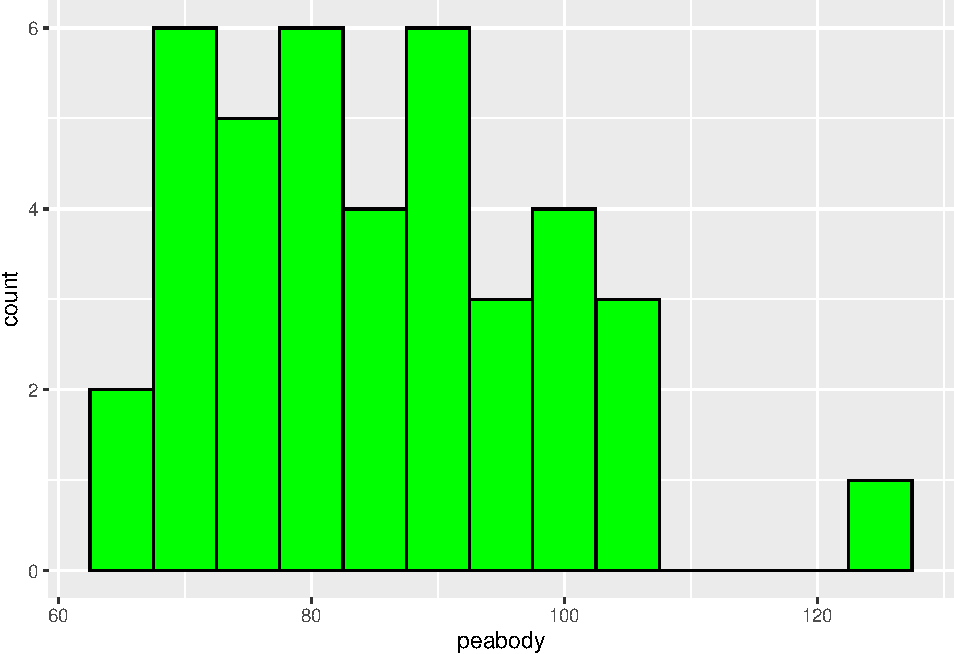
\includegraphics{PSY202A-Modeling-I.Heo_files/figure-latex/unnamed-chunk-77-1.pdf}

\begin{itemize}
\item
  Alternatively, you could set the total number of bins with the \texttt{bins} argument.
\item
  Sometimes you want to display plots for a subset of your data. This can be accomplished using the \texttt{facet\_wrap()} function.
\end{itemize}

\begin{Shaded}
\begin{Highlighting}[]
\FunctionTok{ggplot}\NormalTok{(}\AttributeTok{data =}\NormalTok{ peabody\_tib, }\FunctionTok{aes}\NormalTok{(peabody)) }\SpecialCharTok{+}
  \FunctionTok{geom\_histogram}\NormalTok{(}\AttributeTok{color =} \StringTok{"black"}\NormalTok{, }\AttributeTok{fill =} \StringTok{"green"}\NormalTok{, }
                 \AttributeTok{binwidth =} \DecValTok{5}\NormalTok{) }\SpecialCharTok{+}
  \FunctionTok{facet\_wrap}\NormalTok{(}\SpecialCharTok{\textasciitilde{}}\NormalTok{gender, }\AttributeTok{nrow =} \DecValTok{1}\NormalTok{)}
\end{Highlighting}
\end{Shaded}

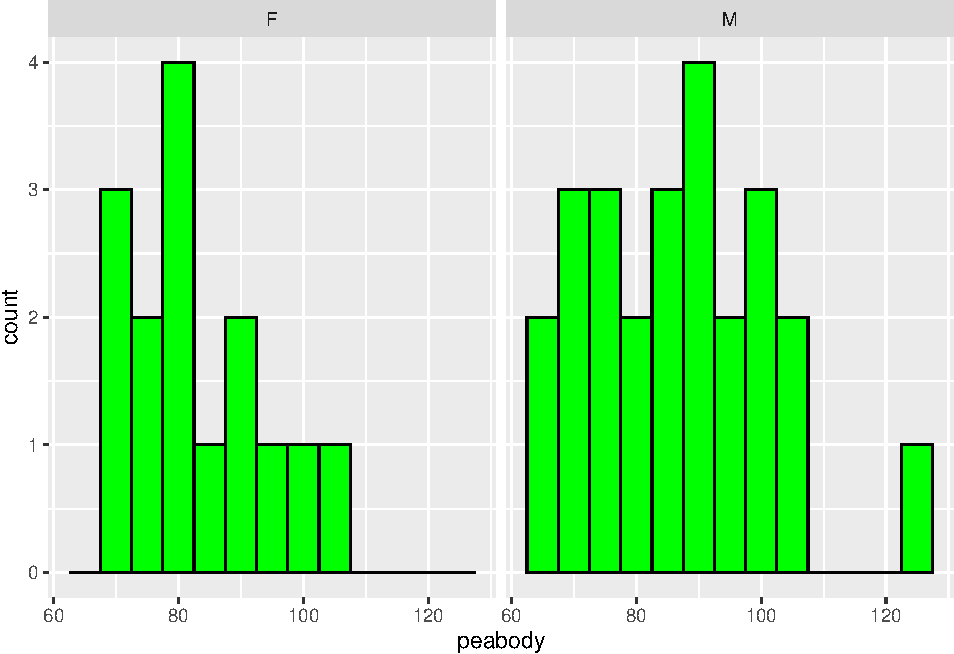
\includegraphics{PSY202A-Modeling-I.Heo_files/figure-latex/unnamed-chunk-78-1.pdf}

\subsection{Bar charts}\label{bar-charts}

\begin{itemize}
\tightlist
\item
  Bar charts are a useful method for displaying categorical data. They can show the number of cases in each of the categories.
\end{itemize}

\begin{Shaded}
\begin{Highlighting}[]
\FunctionTok{ggplot}\NormalTok{(}\AttributeTok{data =}\NormalTok{ peabody\_tib, }\FunctionTok{aes}\NormalTok{(gender)) }\SpecialCharTok{+}
  \FunctionTok{geom\_bar}\NormalTok{(}\AttributeTok{color =} \StringTok{"black"}\NormalTok{, }\AttributeTok{fill =} \FunctionTok{c}\NormalTok{(}\StringTok{"purple"}\NormalTok{,}\StringTok{"green"}\NormalTok{))}
\end{Highlighting}
\end{Shaded}

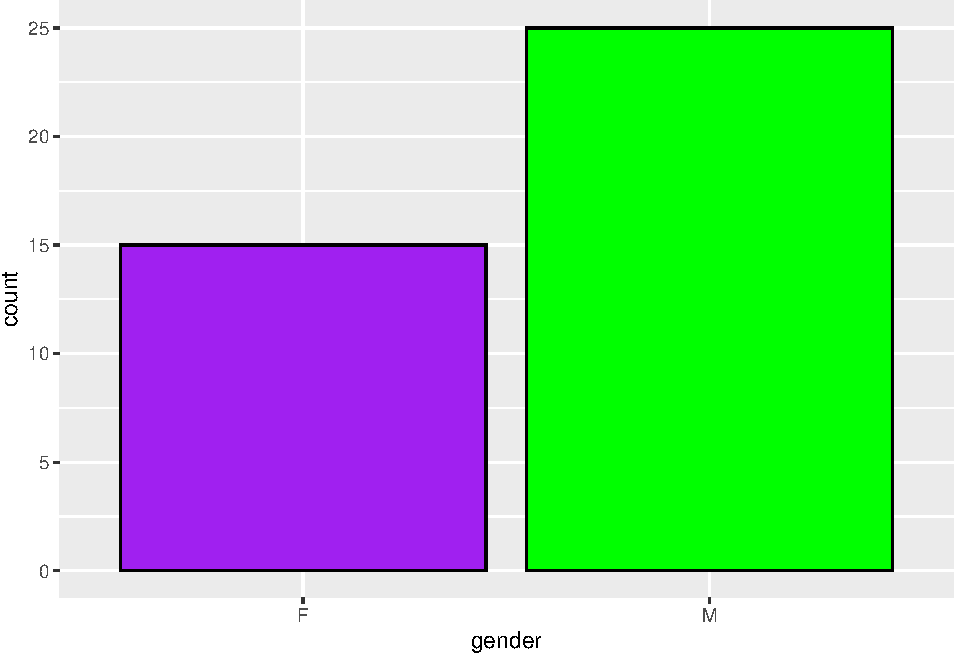
\includegraphics{PSY202A-Modeling-I.Heo_files/figure-latex/unnamed-chunk-79-1.pdf}

\begin{itemize}
\tightlist
\item
  Perhaps you would like to change the \texttt{F} to Female and the \texttt{M} to Male. The x-axis ticks can be changed using the following trick:
\end{itemize}

\begin{Shaded}
\begin{Highlighting}[]
\FunctionTok{ggplot}\NormalTok{(}\AttributeTok{data =}\NormalTok{ peabody\_tib, }\FunctionTok{aes}\NormalTok{(gender)) }\SpecialCharTok{+}
  \FunctionTok{geom\_bar}\NormalTok{(}\AttributeTok{color =} \StringTok{"black"}\NormalTok{, }\AttributeTok{fill =} \FunctionTok{c}\NormalTok{(}\StringTok{"purple"}\NormalTok{,}\StringTok{"green"}\NormalTok{)) }\SpecialCharTok{+}
  \FunctionTok{scale\_x\_discrete}\NormalTok{(}\AttributeTok{labels =} \FunctionTok{c}\NormalTok{(}\StringTok{"Female"}\NormalTok{, }\StringTok{"Male"}\NormalTok{)) }\DocumentationTok{\#\# Changes the labels on the x{-}axis ticks}
\end{Highlighting}
\end{Shaded}

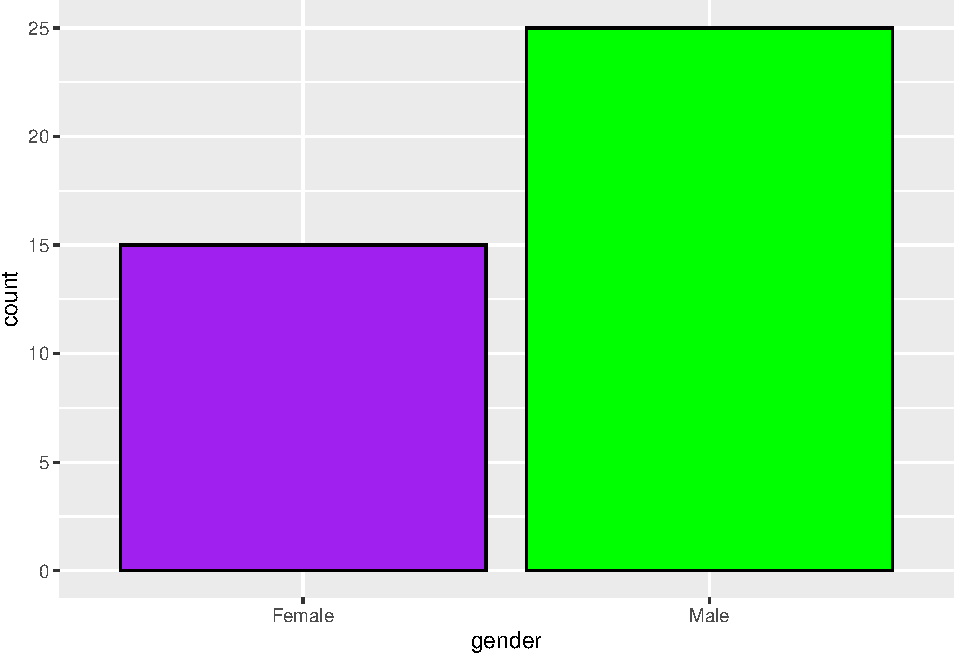
\includegraphics{PSY202A-Modeling-I.Heo_files/figure-latex/unnamed-chunk-80-1.pdf}

\begin{itemize}
\tightlist
\item
  Sometimes it can be helpful to change the plot title, x-axis and y-axis.
\end{itemize}

\begin{Shaded}
\begin{Highlighting}[]
\FunctionTok{ggplot}\NormalTok{(}\AttributeTok{data =}\NormalTok{ peabody\_tib, }\FunctionTok{aes}\NormalTok{(gender)) }\SpecialCharTok{+} 
  \FunctionTok{geom\_bar}\NormalTok{(}\AttributeTok{color =} \StringTok{"black"}\NormalTok{, }\AttributeTok{fill =} \FunctionTok{c}\NormalTok{(}\StringTok{"purple"}\NormalTok{,}\StringTok{"green"}\NormalTok{)) }\SpecialCharTok{+}
  \FunctionTok{scale\_x\_discrete}\NormalTok{(}\AttributeTok{labels =} \FunctionTok{c}\NormalTok{(}\StringTok{"Female"}\NormalTok{, }\StringTok{"Male"}\NormalTok{)) }\SpecialCharTok{+}
  \FunctionTok{labs}\NormalTok{(}\AttributeTok{x=}\StringTok{\textquotesingle{}Gender\textquotesingle{}}\NormalTok{,}
       \AttributeTok{y=}\StringTok{\textquotesingle{}Count of Children\textquotesingle{}}\NormalTok{,}
       \AttributeTok{title=}\StringTok{\textquotesingle{}Gender Breakdown of Children\textquotesingle{}}\NormalTok{) }\DocumentationTok{\#\# Allows you to change the title and axis labels}
\end{Highlighting}
\end{Shaded}

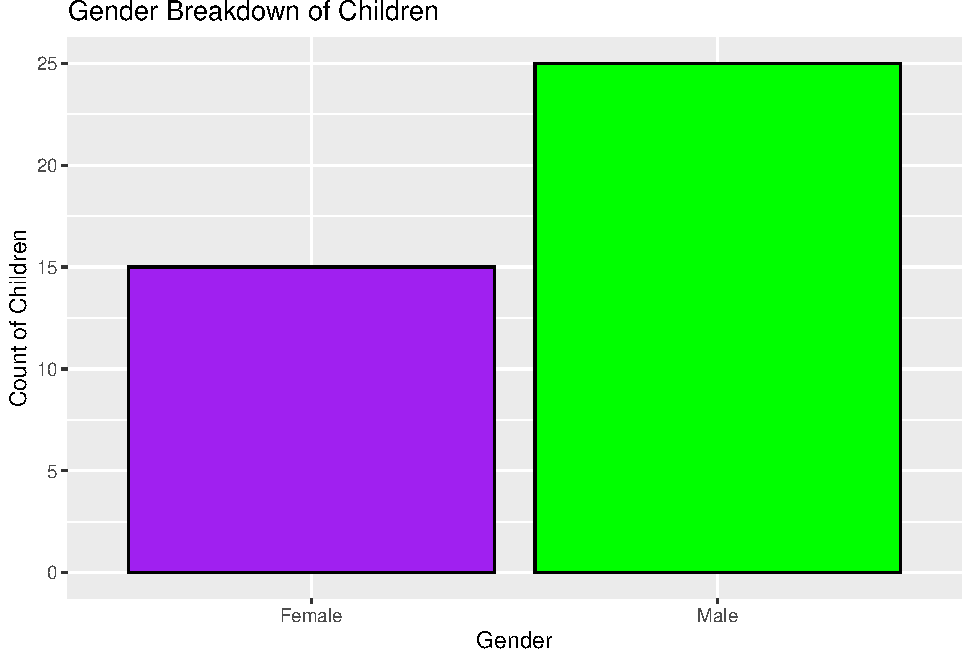
\includegraphics{PSY202A-Modeling-I.Heo_files/figure-latex/unnamed-chunk-81-1.pdf}

\subsection{Scatterplots}\label{scatterplots}

\begin{itemize}
\tightlist
\item
  Scatterplots are a useful method for visualizing the relationship between two numerical variables. We will not discuss how to interpret the scatterplot today, but I thought it might be helpful for you to see how the \texttt{geom\_point()} function works.
\end{itemize}

\begin{Shaded}
\begin{Highlighting}[]
\FunctionTok{ggplot}\NormalTok{(}\AttributeTok{data =}\NormalTok{ peabody\_tib, }\FunctionTok{aes}\NormalTok{(peabody,age)) }\SpecialCharTok{+}
  \FunctionTok{geom\_point}\NormalTok{(}\AttributeTok{shape =} \DecValTok{19}\NormalTok{, }\AttributeTok{size =} \FloatTok{2.5}\NormalTok{, }\AttributeTok{color =} \StringTok{"cyan3"}\NormalTok{)}
\end{Highlighting}
\end{Shaded}

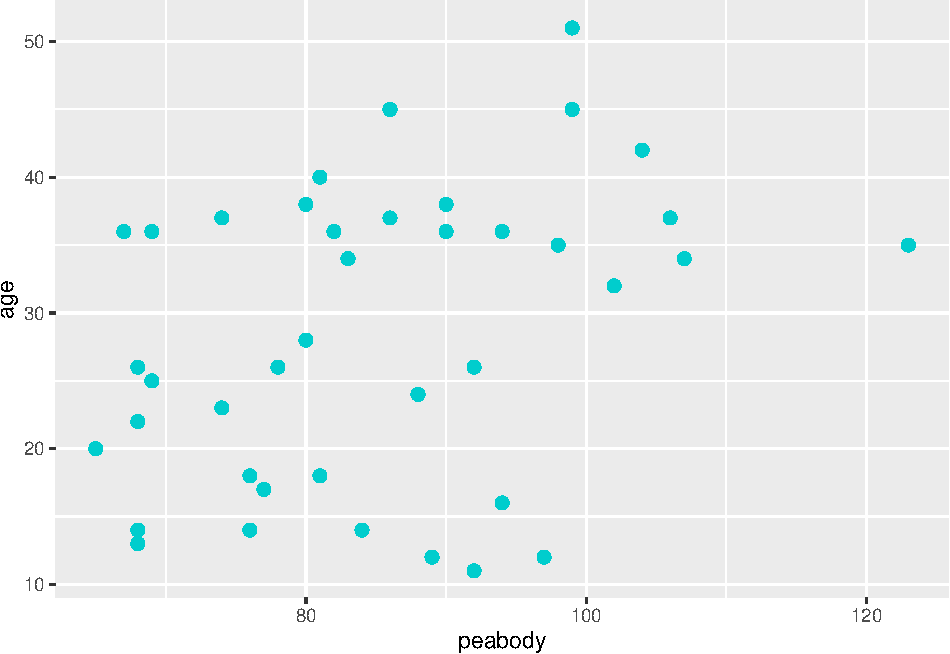
\includegraphics{PSY202A-Modeling-I.Heo_files/figure-latex/unnamed-chunk-82-1.pdf}

\subsection{Important points about data visualization}\label{important-points-about-data-visualization}

\begin{itemize}
\item
  At its core, the term `data visualization' refers to any visual display of data that helps us understand the underlying data better.
\item
  Generally, there are a few charactersitics of all godo plots {[}Note: This is not an exhaustive list{]}.

  \begin{itemize}
  \tightlist
  \item
    Clearly-labeled axes.
  \item
    Text that are large enough to see.
  \item
    Axes that are not misleading.
  \item
    Data that are displayed appropriately considering the type of data you have.
  \end{itemize}
\end{itemize}

\section{Final exercise}\label{final-exercise-2}

\begin{itemize}
\item
  Using the age variable, find the following summary statistics:

  \begin{itemize}
  \tightlist
  \item
    mean
  \item
    median
  \item
    standard deviation
  \item
    skewness
  \item
    kurtosis
  \end{itemize}
\item
  Using the age variable, create a histogram with the following features:

  \begin{itemize}
  \tightlist
  \item
    colored bars.
  \item
    10 bins {[}Hint: use \texttt{bins} argument{]}.
  \item
    a title of ``Age of Children (in months)'' {[}Hint: use \texttt{labs()} function{]}.
  \end{itemize}
\end{itemize}

\chapter{Regression and ANOVA}\label{regression-and-anova}

\section{Your first Ph.D.~statistics course is almost done}\label{your-first-ph.d.-statistics-course-is-almost-done}

\begin{itemize}
\tightlist
\item
  Keep up the excellent work! You're nearly there!
\end{itemize}

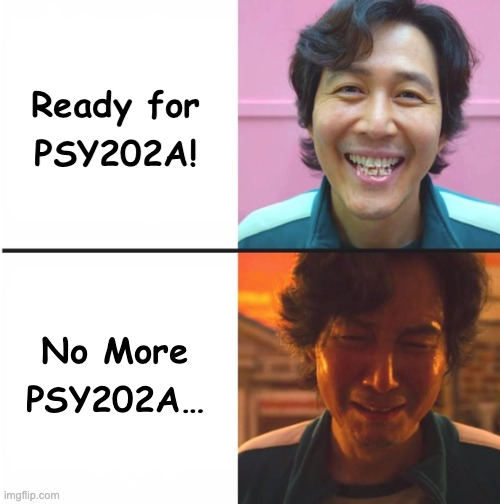
\includegraphics{./img/nopsy202a.png}

\subsection{Regression vs.~ANOVA}\label{regression-vs.-anova}


\includegraphics{./img/regression_anova_meme.png}

\begin{itemize}
\item
  In general, remember that both regression and ANOVA are part of the broader class of general linear models.
\item
  The term `general linear model' refers to conventional linear regression models for a continuous response variable given continuous and/or categorical predictors.

  \begin{itemize}
  \item
    For your information, the term `generalized linear model' refers to a larger class of models that is assumed to follow an exponential family distribution. See \url{https://online.stat.psu.edu/stat504/lesson/6/6.1}.
  \item
    For your additional information, the term `generalized linear mixed model' refers to an even further extension of general linear models that permis random effects as well as fixed effects in the linear predictor. See \url{https://online.stat.psu.edu/stat504/lesson/generalized-linear-mixed-models}.
  \end{itemize}
\item
  Out of curiosity\ldots{} are you familiar with ANCOVA\ldots?
\end{itemize}

\section{What Do We Do Today?}\label{what-do-we-do-today}

\subsection{Goals}\label{goals}

\begin{itemize}
\item
  HW7 (one-way ANOVA) and HW8 (factorial ANOVA) are upcoming. Therefore, we will first discuss ANOVA, focusing on helping you succeed with these assignments.
\item
  We will also discuss regression analysis. Let's approach it with a relaxed and review-oriented mindset.
\end{itemize}

\subsection{Packages}\label{packages-2}

\begin{itemize}
\tightlist
\item
  Initial setting
\end{itemize}

\begin{Shaded}
\begin{Highlighting}[]
\CommentTok{\# Clean the workspace}
\FunctionTok{rm}\NormalTok{(}\AttributeTok{list=}\FunctionTok{ls}\NormalTok{());}\FunctionTok{gc}\NormalTok{()}
\end{Highlighting}
\end{Shaded}

\begin{verbatim}
##           used (Mb) gc trigger  (Mb) limit (Mb) max used  (Mb)
## Ncells 1444103 77.2    2204455 117.8         NA  2204455 117.8
## Vcells 2532243 19.4    8388608  64.0      16384  4387670  33.5
\end{verbatim}

\begin{Shaded}
\begin{Highlighting}[]
\CommentTok{\# Set the working directory}
\FunctionTok{setwd}\NormalTok{(}\StringTok{"/Users/ihnwhiheo/Github/PSY202A\_Modeling"}\NormalTok{)}
\FunctionTok{getwd}\NormalTok{()}
\end{Highlighting}
\end{Shaded}

\begin{verbatim}
## [1] "/Users/ihnwhiheo/Github/PSY202A_Modeling"
\end{verbatim}

\begin{itemize}
\tightlist
\item
  Let's load R packages that will be used throughout.
\end{itemize}

\begin{Shaded}
\begin{Highlighting}[]
\CommentTok{\# List of packages}
\NormalTok{packages }\OtherTok{\textless{}{-}} \FunctionTok{c}\NormalTok{(}\StringTok{"psych"}\NormalTok{, }\StringTok{"QuantPsyc"}\NormalTok{, }\StringTok{"car"}\NormalTok{, }\StringTok{"apaTables"}\NormalTok{, }\StringTok{"report"}\NormalTok{, }\StringTok{"multcomp"}\NormalTok{,}
              \StringTok{"palmerpenguins"}\NormalTok{, }\StringTok{"tidyverse"}\NormalTok{, }\StringTok{"ggformula"}\NormalTok{, }\StringTok{"emmeans"}\NormalTok{) }\CommentTok{\# Add the package names you need}

\CommentTok{\# Check, install, and load each package}
\ControlFlowTok{for}\NormalTok{ (package\_name }\ControlFlowTok{in}\NormalTok{ packages) \{}
  \ControlFlowTok{if}\NormalTok{ (}\SpecialCharTok{!}\FunctionTok{requireNamespace}\NormalTok{(package\_name, }\AttributeTok{quietly =} \ConstantTok{TRUE}\NormalTok{)) \{}
    \FunctionTok{install.packages}\NormalTok{(package\_name, }\AttributeTok{dependencies =} \ConstantTok{TRUE}\NormalTok{)}
\NormalTok{  \}}
  \FunctionTok{library}\NormalTok{(package\_name, }\AttributeTok{character.only =} \ConstantTok{TRUE}\NormalTok{)}
\NormalTok{\}}
\end{Highlighting}
\end{Shaded}

\begin{verbatim}
## Warning: package 'ggformula' was built under R version 4.2.3
\end{verbatim}

\begin{verbatim}
## Warning: package 'scales' was built under R version 4.2.3
\end{verbatim}

\begin{verbatim}
## Warning: package 'ggridges' was built under R version 4.2.3
\end{verbatim}

\begin{itemize}
\tightlist
\item
  We will be using with the \texttt{sat.act} dataset in the R \texttt{psych} package.

  \begin{itemize}
  \tightlist
  \item
    The dataset consists of self-reported scores of 700 subjects on the SAT Verbal, SAT Quantitative and ACT. Additional variables include age, gender (0=female, 1=male), and education ().
  \end{itemize}
\end{itemize}

\begin{Shaded}
\begin{Highlighting}[]
\CommentTok{\# Load data}
\FunctionTok{data}\NormalTok{(sat.act)}
\NormalTok{dat }\OtherTok{\textless{}{-}}\NormalTok{ sat.act}
\end{Highlighting}
\end{Shaded}

\begin{itemize}
\item
  In the original dataset, gender is coded as 1 for males and 2 for females.
\item
  The education variable is categorical, ranging from 1 (high school) to 5 (graduate work). For the variables coded as 0, I could not find the exact coding scheme, so we assume that 0 refers to no education.
\item
  While the other variables are continuous and require no data preprocessing, we will perform some quick data engineering for gender and education.
\item
  Specifically, we will recode gender so that females (originally coded as 2) become the reference category by assigning them a value of 0. Additionally, we will treat the education variable as categorical.
\end{itemize}

\begin{Shaded}
\begin{Highlighting}[]
\CommentTok{\# Data engineering}
\NormalTok{dat}\SpecialCharTok{$}\NormalTok{gender\_original }\OtherTok{\textless{}{-}}\NormalTok{ dat}\SpecialCharTok{$}\NormalTok{gender}
\NormalTok{dat}\SpecialCharTok{$}\NormalTok{gender }\OtherTok{\textless{}{-}} \FunctionTok{ifelse}\NormalTok{(dat}\SpecialCharTok{$}\NormalTok{gender }\SpecialCharTok{==} \DecValTok{1}\NormalTok{, }\DecValTok{1}\NormalTok{, }\DecValTok{0}\NormalTok{)}
\NormalTok{dat}\SpecialCharTok{$}\NormalTok{education }\OtherTok{\textless{}{-}} \FunctionTok{as.factor}\NormalTok{(dat}\SpecialCharTok{$}\NormalTok{education)}

\CommentTok{\# Quick overview of the data}
\FunctionTok{head}\NormalTok{(dat, }\DecValTok{20}\NormalTok{)}
\end{Highlighting}
\end{Shaded}

\begin{verbatim}
##       gender education age ACT SATV SATQ gender_original
## 29442      0         3  19  24  500  500               2
## 29457      0         3  23  35  600  500               2
## 29498      0         3  20  21  480  470               2
## 29503      1         4  27  26  550  520               1
## 29504      1         2  33  31  600  550               1
## 29518      1         5  26  28  640  640               1
## 29527      0         5  30  36  610  500               2
## 29529      1         3  19  22  520  560               1
## 29543      0         4  23  22  400  600               2
## 29547      0         5  40  35  730  800               2
## 29578      1         3  23  32  760  710               1
## 29592      0         4  34  29  710  600               2
## 29617      1         4  32  21  600  600               1
## 29619      0         4  41  35  780  725               2
## 29633      0         3  20  27  640  630               2
## 29671      0         4  24  27  640  590               2
## 29676      0         3  19  33  640  650               2
## 29685      0         4  24  32  700  620               2
## 29710      1         4  35  28  640  580               1
## 29711      0         4  46  32  610  680               2
\end{verbatim}

\begin{itemize}
\tightlist
\item
  Shall we look at the descriptive statistics?
\end{itemize}

\begin{Shaded}
\begin{Highlighting}[]
\CommentTok{\# Descriptive statistics}
\FunctionTok{describe}\NormalTok{(dat)}
\end{Highlighting}
\end{Shaded}

\begin{verbatim}
##                 vars   n   mean     sd median trimmed    mad min max range
## gender             1 700   0.35   0.48      0    0.32   0.00   0   1     1
## education*         2 700   4.16   1.43      4    4.31   1.48   1   6     5
## age                3 700  25.59   9.50     22   23.86   5.93  13  65    52
## ACT                4 700  28.55   4.82     29   28.84   4.45   3  36    33
## SATV               5 700 612.23 112.90    620  619.45 118.61 200 800   600
## SATQ               6 687 610.22 115.64    620  617.25 118.61 200 800   600
## gender_original    7 700   1.65   0.48      2    1.68   0.00   1   2     1
##                  skew kurtosis   se
## gender           0.61    -1.62 0.02
## education*      -0.68    -0.07 0.05
## age              1.64     2.42 0.36
## ACT             -0.66     0.53 0.18
## SATV            -0.64     0.33 4.27
## SATQ            -0.59    -0.02 4.41
## gender_original -0.61    -1.62 0.02
\end{verbatim}

\begin{itemize}
\tightlist
\item
  For categorical variables (i.e., gender and education), let's make a table and view the frequencies.
\end{itemize}

\begin{Shaded}
\begin{Highlighting}[]
\CommentTok{\# Descriptive statistics}
\NormalTok{tab }\OtherTok{\textless{}{-}} \FunctionTok{table}\NormalTok{(}\AttributeTok{Gender =}\NormalTok{ dat}\SpecialCharTok{$}\NormalTok{gender, }\AttributeTok{Education =}\NormalTok{ dat}\SpecialCharTok{$}\NormalTok{education)}
\FunctionTok{addmargins}\NormalTok{(tab)}
\end{Highlighting}
\end{Shaded}

\begin{verbatim}
##       Education
## Gender   0   1   2   3   4   5 Sum
##    0    30  25  21 195  87  95 453
##    1    27  20  23  80  51  46 247
##    Sum  57  45  44 275 138 141 700
\end{verbatim}

\section{One-way ANOVA}\label{one-way-anova}

\subsection{Assumptions}\label{assumptions}

\begin{quote}
Trailer: You will literally enjoy assumptions in PSY202B with Sarah!
\end{quote}

\begin{enumerate}
\def\labelenumi{\arabic{enumi}.}
\tightlist
\item
  Normality: We assume that the populations from which the samples were taken are normally distributed.
\end{enumerate}

\begin{itemize}
\tightlist
\item
  Numerically, we can check the skewness and kurtosis of the variables. For instance,
\end{itemize}

\begin{Shaded}
\begin{Highlighting}[]
\CommentTok{\# Skewness and kurtosis}
\FunctionTok{skew}\NormalTok{(dat}\SpecialCharTok{$}\NormalTok{ACT) }\CommentTok{\# Little bit negatively skewed (if 0, no skew; if positive, positively skewed)}
\end{Highlighting}
\end{Shaded}

\begin{verbatim}
## [1] -0.6564026
\end{verbatim}

\begin{Shaded}
\begin{Highlighting}[]
\FunctionTok{kurtosi}\NormalTok{(dat}\SpecialCharTok{$}\NormalTok{ACT) }\CommentTok{\# Little bit leptokurtic (if 0, mesokurti;, if negative, platykurtic)}
\end{Highlighting}
\end{Shaded}

\begin{verbatim}
## [1] 0.5349691
\end{verbatim}

\begin{itemize}
\tightlist
\item
  Visually, we can check the QQ plot. For instance:
\end{itemize}

\begin{Shaded}
\begin{Highlighting}[]
\CommentTok{\# QQ plot}
\FunctionTok{qqnorm}\NormalTok{(dat}\SpecialCharTok{$}\NormalTok{ACT)}
\FunctionTok{qqline}\NormalTok{(dat}\SpecialCharTok{$}\NormalTok{ACT)}
\end{Highlighting}
\end{Shaded}

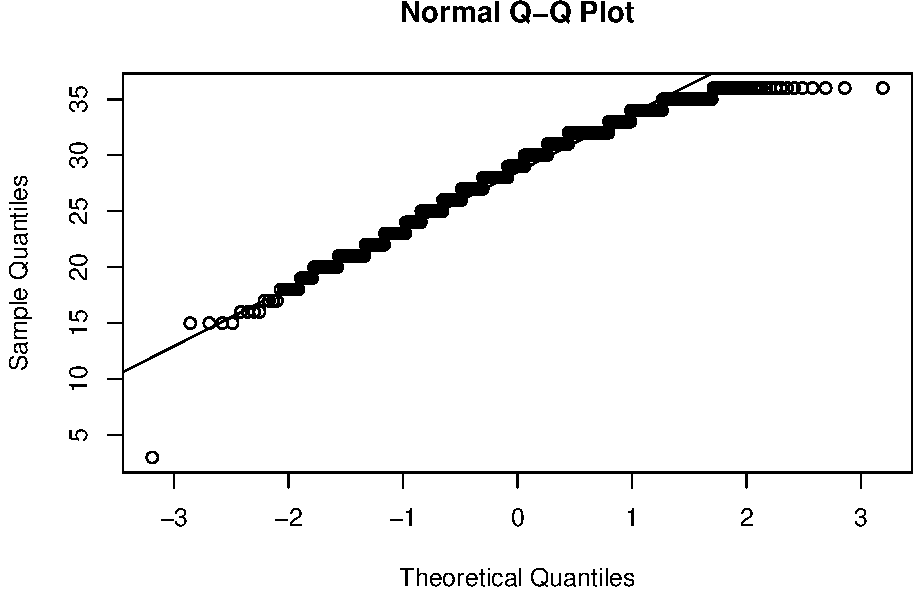
\includegraphics{PSY202A-Modeling-I.Heo_files/figure-latex/unnamed-chunk-90-1.pdf}

\begin{itemize}
\tightlist
\item
  Or simply we can check the histogram.
\end{itemize}

\begin{Shaded}
\begin{Highlighting}[]
\CommentTok{\# Histogram}
\FunctionTok{hist}\NormalTok{(dat}\SpecialCharTok{$}\NormalTok{ACT)}
\end{Highlighting}
\end{Shaded}

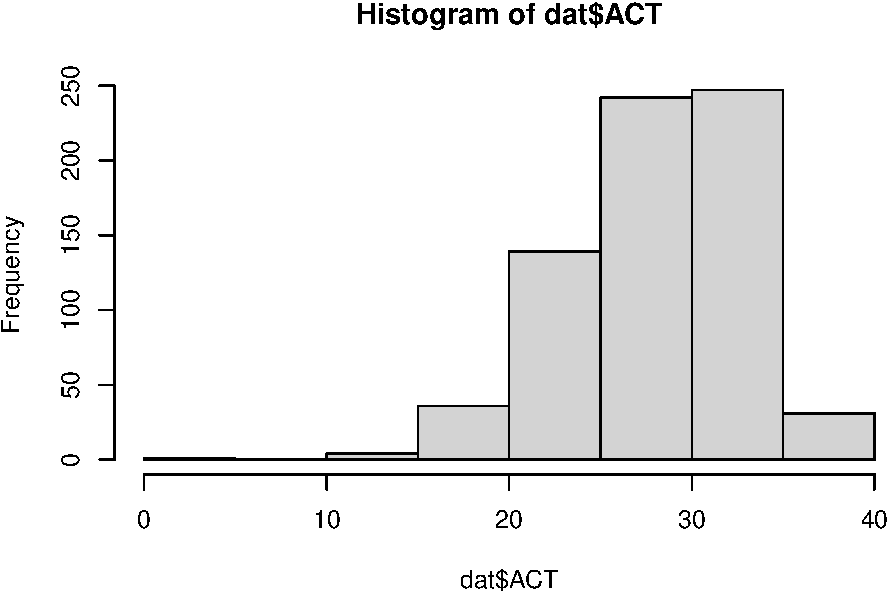
\includegraphics{PSY202A-Modeling-I.Heo_files/figure-latex/unnamed-chunk-91-1.pdf}

\begin{itemize}
\tightlist
\item
  Or we can examine the density plot to compare the distribution of the variable against the ideal normal distribution.
\end{itemize}

\begin{Shaded}
\begin{Highlighting}[]
\CommentTok{\# Density plot}
\FunctionTok{plotNormX}\NormalTok{(dat}\SpecialCharTok{$}\NormalTok{ACT)}
\end{Highlighting}
\end{Shaded}

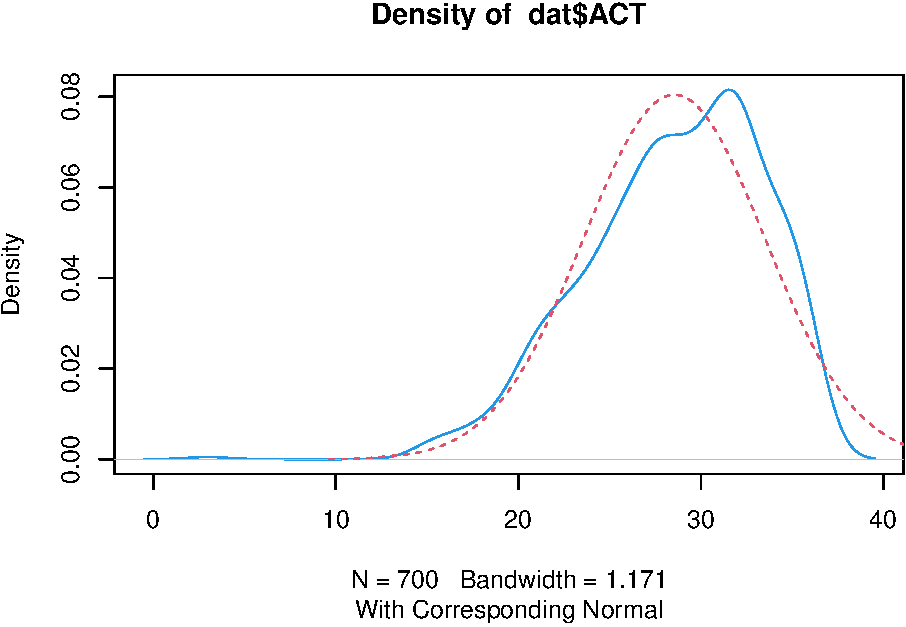
\includegraphics{PSY202A-Modeling-I.Heo_files/figure-latex/unnamed-chunk-92-1.pdf}

\begin{enumerate}
\def\labelenumi{\arabic{enumi}.}
\setcounter{enumi}{1}
\tightlist
\item
  Random sampling: We assume that the data we measure were obtained from a sample that we selected using a random sampling procedure.
\end{enumerate}

\begin{itemize}
\tightlist
\item
  We cannot statistically test whether random sampling has occurred. Think about the data collection method you used.
\end{itemize}

\begin{enumerate}
\def\labelenumi{\arabic{enumi}.}
\setcounter{enumi}{2}
\tightlist
\item
  Independence: We assume that the probabilities of each measured outcome in a study are independent or equal.
\end{enumerate}

\begin{itemize}
\tightlist
\item
  For the independence assumption, we cannot test this statistically. Just think about the data collection method you used.
\end{itemize}

\begin{enumerate}
\def\labelenumi{\arabic{enumi}.}
\setcounter{enumi}{3}
\tightlist
\item
  Homogeneity of variance (i.e., homoscedasticity): We assume that the samples were drawn from populations of equal variances.
\end{enumerate}

\begin{itemize}
\item
  Numerically, we can conduct Barlett's or Levene's test.

  \begin{itemize}
  \tightlist
  \item
    If significant, the assumption of homogeneity of variances is violated.
  \end{itemize}
\end{itemize}

\begin{Shaded}
\begin{Highlighting}[]
\CommentTok{\# Bartlett\textquotesingle{}s test}
\FunctionTok{bartlett.test}\NormalTok{(ACT }\SpecialCharTok{\textasciitilde{}}\NormalTok{ gender, }\AttributeTok{data =}\NormalTok{ dat)}
\end{Highlighting}
\end{Shaded}

\begin{verbatim}
## 
##  Bartlett test of homogeneity of variances
## 
## data:  ACT by gender
## Bartlett's K-squared = 1.9164, df = 1, p-value = 0.1663
\end{verbatim}

\begin{Shaded}
\begin{Highlighting}[]
\FunctionTok{bartlett.test}\NormalTok{(ACT }\SpecialCharTok{\textasciitilde{}}\NormalTok{ education, }\AttributeTok{data =}\NormalTok{ dat)}
\end{Highlighting}
\end{Shaded}

\begin{verbatim}
## 
##  Bartlett test of homogeneity of variances
## 
## data:  ACT by education
## Bartlett's K-squared = 21.624, df = 5, p-value = 0.0006172
\end{verbatim}

\begin{Shaded}
\begin{Highlighting}[]
\CommentTok{\# Levene\textquotesingle{}s test}
\FunctionTok{leveneTest}\NormalTok{(dat}\SpecialCharTok{$}\NormalTok{ACT, }\AttributeTok{group =}\NormalTok{ dat}\SpecialCharTok{$}\NormalTok{gender)}
\end{Highlighting}
\end{Shaded}

\begin{verbatim}
## Warning in leveneTest.default(dat$ACT, group = dat$gender): dat$gender coerced
## to factor.
\end{verbatim}

\begin{verbatim}
## Levene's Test for Homogeneity of Variance (center = median)
##        Df F value Pr(>F)
## group   1  0.2899 0.5904
##       698
\end{verbatim}

\begin{Shaded}
\begin{Highlighting}[]
\FunctionTok{leveneTest}\NormalTok{(dat}\SpecialCharTok{$}\NormalTok{ACT, }\AttributeTok{group =}\NormalTok{ dat}\SpecialCharTok{$}\NormalTok{education)}
\end{Highlighting}
\end{Shaded}

\begin{verbatim}
## Levene's Test for Homogeneity of Variance (center = median)
##        Df F value   Pr(>F)   
## group   5   3.279 0.006194 **
##       694                    
## ---
## Signif. codes:  0 '***' 0.001 '**' 0.01 '*' 0.05 '.' 0.1 ' ' 1
\end{verbatim}

\begin{itemize}
\tightlist
\item
  Visually, we can look at the box plots
\end{itemize}

\begin{Shaded}
\begin{Highlighting}[]
\CommentTok{\# Boxplots}
\FunctionTok{boxplot}\NormalTok{(ACT }\SpecialCharTok{\textasciitilde{}}\NormalTok{ gender, }\AttributeTok{data =}\NormalTok{ dat)}
\end{Highlighting}
\end{Shaded}

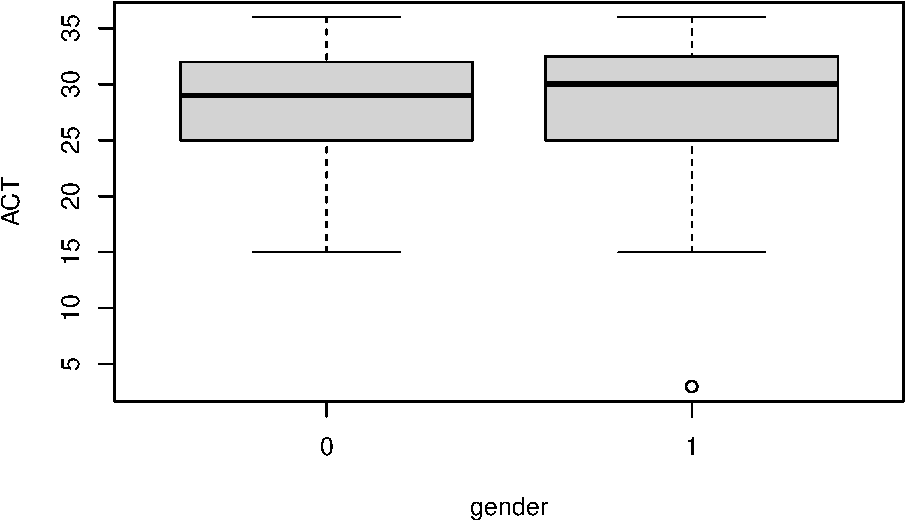
\includegraphics{PSY202A-Modeling-I.Heo_files/figure-latex/unnamed-chunk-94-1.pdf}

\begin{Shaded}
\begin{Highlighting}[]
\FunctionTok{boxplot}\NormalTok{(ACT }\SpecialCharTok{\textasciitilde{}}\NormalTok{ education, }\AttributeTok{data =}\NormalTok{ dat)}
\end{Highlighting}
\end{Shaded}

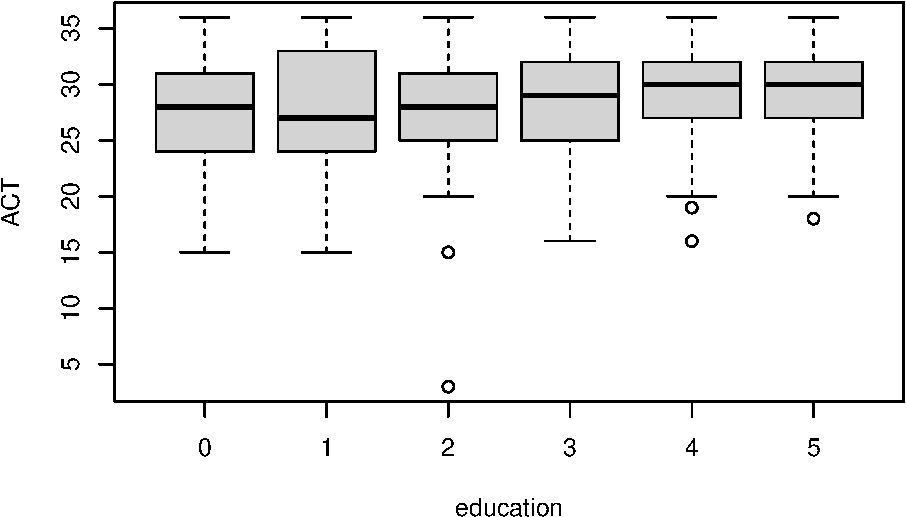
\includegraphics{PSY202A-Modeling-I.Heo_files/figure-latex/unnamed-chunk-94-2.pdf}

\subsection{Analysis}\label{analysis}

\begin{itemize}
\tightlist
\item
  Let's conduct a one-way ANOVA to test whether there are significant mean differences in ACT scores across the different education levels.
\end{itemize}

\begin{Shaded}
\begin{Highlighting}[]
\CommentTok{\# Perform a one{-}way ANOVA}
\NormalTok{model\_oaov }\OtherTok{\textless{}{-}} \FunctionTok{aov}\NormalTok{(ACT }\SpecialCharTok{\textasciitilde{}}\NormalTok{ education, }\AttributeTok{data =}\NormalTok{ dat)}

\CommentTok{\# Print the output}
\FunctionTok{summary}\NormalTok{(model\_oaov)}
\end{Highlighting}
\end{Shaded}

\begin{verbatim}
##              Df Sum Sq Mean Sq F value  Pr(>F)   
## education     5    470   93.90   4.126 0.00106 **
## Residuals   694  15794   22.76                   
## ---
## Signif. codes:  0 '***' 0.001 '**' 0.01 '*' 0.05 '.' 0.1 ' ' 1
\end{verbatim}

\begin{Shaded}
\begin{Highlighting}[]
\CommentTok{\# Make the APA{-}style table}
\FunctionTok{apa.aov.table}\NormalTok{(model\_oaov)}
\end{Highlighting}
\end{Shaded}

\begin{verbatim}
## 
## 
## ANOVA results using ACT as the dependent variable
##  
## 
##    Predictor       SS  df       MS       F    p partial_eta2 CI_90_partial_eta2
##  (Intercept) 43023.79   1 43023.79 1890.50 .000                                
##    education   469.50   5    93.90    4.13 .001          .03         [.01, .05]
##        Error 15793.94 694    22.76                                             
## 
## Note: Values in square brackets indicate the bounds of the 90% confidence interval for partial eta-squared
\end{verbatim}

\begin{Shaded}
\begin{Highlighting}[]
\CommentTok{\# Describe the result following the APA{-}style; but for reference ONLY!}
\FunctionTok{report}\NormalTok{(model\_oaov)}
\end{Highlighting}
\end{Shaded}

\begin{verbatim}
## The ANOVA (formula: ACT ~ education) suggests that:
## 
##   - The main effect of education is statistically significant and small (F(5,
## 694) = 4.13, p = 0.001; Eta2 = 0.03, 95% CI [7.33e-03, 1.00])
## 
## Effect sizes were labelled following Field's (2013) recommendations.
\end{verbatim}

\subsection{Can you explain to me how those results have been obtained?}\label{can-you-explain-to-me-how-those-results-have-been-obtained}

\begin{itemize}
\tightlist
\item
  I'll leave this as food for thought for you!
\end{itemize}

\subsection{How can we interpret the results?}\label{how-can-we-interpret-the-results}

\begin{itemize}
\tightlist
\item
  According to the ANOVA summary table, the omnibus F-test is statistically significant, as the p-value is below the alpha level of 0.05. This indicates that the null hypothesis of equal population means across the six education groups is rejected. Consequently, we conclude that the six education levels are associated with different ACT scores.
\end{itemize}

\subsection{Given the results, we are now interested in testing the differences among all the pairs of the means. Because using multiple t-tests can inflate familywise error rates, we will use one of the correction methods. What should we do?}\label{given-the-results-we-are-now-interested-in-testing-the-differences-among-all-the-pairs-of-the-means.-because-using-multiple-t-tests-can-inflate-familywise-error-rates-we-will-use-one-of-the-correction-methods.-what-should-we-do}

\begin{itemize}
\tightlist
\item
  Note that Bonferroni and Holm-Bonferroni are a priori comparison methods. This means they are used when we have a planned set of comparisons before collecting data.

  \begin{itemize}
  \tightlist
  \item
    In our case, we did not have such a plan (or did you have something in mind? If then, you are amazing!). Therefore, we will use either Fisher's LSD or Tukey's HSD for post hoc comparisons.
  \end{itemize}
\item
  Fisher's LSD is typically used when there are only three means to compare. This is because, with three means, the family-wise error rate remains controlled at the significance level of alpha.

  \begin{itemize}
  \tightlist
  \item
    However, when comparing more than three means, the overall F-test does not adequately protect the family-wise error rate if the complete null hypothesis is not true but a subset of it is.
  \end{itemize}
\item
  Tukey's HSD, on the other hand, is specifically designed to perform all possible pairwise comparisons. It ensures that the researcher has only a 5\% chance of finding a significant mean difference when the null hypothesis is true.

  \begin{itemize}
  \tightlist
  \item
    In the current example, there are 15 comparisons to be made (Can you understand why? If yes, please explain that to me!). Thus, Tukey's HSD is the appropriate method among the four correction techniques.
  \end{itemize}
\end{itemize}

\begin{Shaded}
\begin{Highlighting}[]
\CommentTok{\# Tukey\textquotesingle{}s HSD}
\FunctionTok{TukeyHSD}\NormalTok{(model\_oaov)}
\end{Highlighting}
\end{Shaded}

\begin{verbatim}
##   Tukey multiple comparisons of means
##     95% family-wise confidence level
## 
## Fit: aov(formula = ACT ~ education, data = dat)
## 
## $education
##            diff         lwr      upr     p adj
## 1-0  0.01520468 -2.70335124 2.733761 1.0000000
## 2-0 -0.49641148 -3.23217649 2.239354 0.9954530
## 3-0  0.82086124 -1.16316374 2.804886 0.8453156
## 4-0  1.78718535 -0.35927170 3.933642 0.1648941
## 5-0  2.12915267 -0.01061924 4.268925 0.0520133
## 2-1 -0.51161616 -3.40192518 2.378693 0.9959541
## 3-1  0.80565657 -1.38656404 2.997877 0.9005816
## 4-1  1.77198068 -0.56826588 4.112227 0.2562269
## 5-1  2.11394799 -0.22016851 4.448064 0.1015015
## 3-2  1.31727273 -0.89625276 3.530798 0.5317982
## 4-2  2.28359684 -0.07661879 4.643812 0.0644453
## 5-2  2.62556415  0.27142658 4.979702 0.0186900
## 4-3  0.96632411 -0.45584423 2.388492 0.3775325
## 5-3  1.30829142 -0.10376689 2.720350 0.0874803
## 5-4  0.34196731 -1.29046383 1.974398 0.9911202
\end{verbatim}

\begin{Shaded}
\begin{Highlighting}[]
\CommentTok{\# Test whether the adjusted p{-}values are lower than 0.05}
\FunctionTok{TukeyHSD}\NormalTok{(model\_oaov)}\SpecialCharTok{$}\NormalTok{education[,}\DecValTok{4}\NormalTok{] }\SpecialCharTok{\textless{}} \FloatTok{0.05}
\end{Highlighting}
\end{Shaded}

\begin{verbatim}
##   1-0   2-0   3-0   4-0   5-0   2-1   3-1   4-1   5-1   3-2   4-2   5-2   4-3 
## FALSE FALSE FALSE FALSE FALSE FALSE FALSE FALSE FALSE FALSE FALSE  TRUE FALSE 
##   5-3   5-4 
## FALSE FALSE
\end{verbatim}

\begin{itemize}
\tightlist
\item
  The adjusted p-values based on Tukey's HSD indicate a significant difference when comparing the means of group 2 and group 5. Therefore, the group means for 2 and 5 are significantly different.
\end{itemize}

\subsection{Something more about a priori contrasts and post-hoc comparison}\label{something-more-about-a-priori-contrasts-and-post-hoc-comparison}

\begin{itemize}
\item
  For our valuable learning experiences, we can also use other packages for multiple comparisons.
\item
  Let's start with the usage of the \texttt{multcomp} package.
\item
  The \texttt{glht} function is used to create a test for multiple contrasts. The contrasts can be all-possible pairwise comparisons, which is referred to as ``Tukey'' in this package. Then, the result of multiple contrasts can be summarized and adjusted for familywise error rate.
\item
  The Bonferroni method is used in this example. Note that if the test argument is not specified, the single-step approach is used. The adjusted p values is computed from the joint normal or t distribution of the z statistics such that the p value represents the probability of getting at least one significant result by chance if all z or t values are the same in all contrasts. The Tukey method and the single-step approach will provide the same results if the group sizes are equal.
\end{itemize}

\begin{Shaded}
\begin{Highlighting}[]
\CommentTok{\# Multiple comparisons}
\NormalTok{pairwise }\OtherTok{\textless{}{-}} \FunctionTok{glht}\NormalTok{(model\_oaov, }\AttributeTok{linfct =} \FunctionTok{mcp}\NormalTok{(}\AttributeTok{education =} \StringTok{"Tukey"}\NormalTok{))}
\FunctionTok{summary}\NormalTok{(pairwise, }\AttributeTok{test =} \FunctionTok{adjusted}\NormalTok{(}\AttributeTok{type =} \StringTok{"bonferroni"}\NormalTok{))}
\end{Highlighting}
\end{Shaded}

\begin{verbatim}
## 
##   Simultaneous Tests for General Linear Hypotheses
## 
## Multiple Comparisons of Means: Tukey Contrasts
## 
## 
## Fit: aov(formula = ACT ~ education, data = dat)
## 
## Linear Hypotheses:
##            Estimate Std. Error t value Pr(>|t|)  
## 1 - 0 == 0   0.0152     0.9513   0.016   1.0000  
## 2 - 0 == 0  -0.4964     0.9573  -0.519   1.0000  
## 3 - 0 == 0   0.8209     0.6943   1.182   1.0000  
## 4 - 0 == 0   1.7872     0.7511   2.379   0.2642  
## 5 - 0 == 0   2.1292     0.7488   2.844   0.0689 .
## 2 - 1 == 0  -0.5116     1.0114  -0.506   1.0000  
## 3 - 1 == 0   0.8057     0.7671   1.050   1.0000  
## 4 - 1 == 0   1.7720     0.8189   2.164   0.4623  
## 5 - 1 == 0   2.1139     0.8168   2.588   0.1478  
## 3 - 2 == 0   1.3173     0.7746   1.701   1.0000  
## 4 - 2 == 0   2.2836     0.8259   2.765   0.0877 .
## 5 - 2 == 0   2.6256     0.8238   3.187   0.0225 *
## 4 - 3 == 0   0.9663     0.4977   1.942   0.7886  
## 5 - 3 == 0   1.3083     0.4941   2.648   0.1243  
## 5 - 4 == 0   0.3420     0.5712   0.599   1.0000  
## ---
## Signif. codes:  0 '***' 0.001 '**' 0.01 '*' 0.05 '.' 0.1 ' ' 1
## (Adjusted p values reported -- bonferroni method)
\end{verbatim}

\begin{itemize}
\tightlist
\item
  The simultaneous confidence interval can be computed by the \texttt{confint} function:
\end{itemize}

\begin{Shaded}
\begin{Highlighting}[]
\CommentTok{\# Confidence interval}
\FunctionTok{confint}\NormalTok{(pairwise)}
\end{Highlighting}
\end{Shaded}

\begin{verbatim}
## 
##   Simultaneous Confidence Intervals
## 
## Multiple Comparisons of Means: Tukey Contrasts
## 
## 
## Fit: aov(formula = ACT ~ education, data = dat)
## 
## Quantile = 2.829
## 95% family-wise confidence level
##  
## 
## Linear Hypotheses:
##            Estimate lwr      upr     
## 1 - 0 == 0  0.01520 -2.67601  2.70642
## 2 - 0 == 0 -0.49641 -3.20466  2.21184
## 3 - 0 == 0  0.82086 -1.14321  2.78493
## 4 - 0 == 0  1.78719 -0.33769  3.91206
## 5 - 0 == 0  2.12915  0.01090  4.24741
## 2 - 1 == 0 -0.51162 -3.37286  2.34963
## 3 - 1 == 0  0.80566 -1.36452  2.97583
## 4 - 1 == 0  1.77198 -0.54473  4.08869
## 5 - 1 == 0  2.11395 -0.19669  4.42459
## 3 - 2 == 0  1.31727 -0.87399  3.50854
## 4 - 2 == 0  2.28360 -0.05288  4.62008
## 5 - 2 == 0  2.62556  0.29510  4.95603
## 4 - 3 == 0  0.96632 -0.44154  2.37419
## 5 - 3 == 0  1.30829 -0.08957  2.70615
## 5 - 4 == 0  0.34197 -1.27405  1.95798
\end{verbatim}

\begin{Shaded}
\begin{Highlighting}[]
\FunctionTok{plot}\NormalTok{(}\FunctionTok{confint}\NormalTok{(pairwise))}
\end{Highlighting}
\end{Shaded}

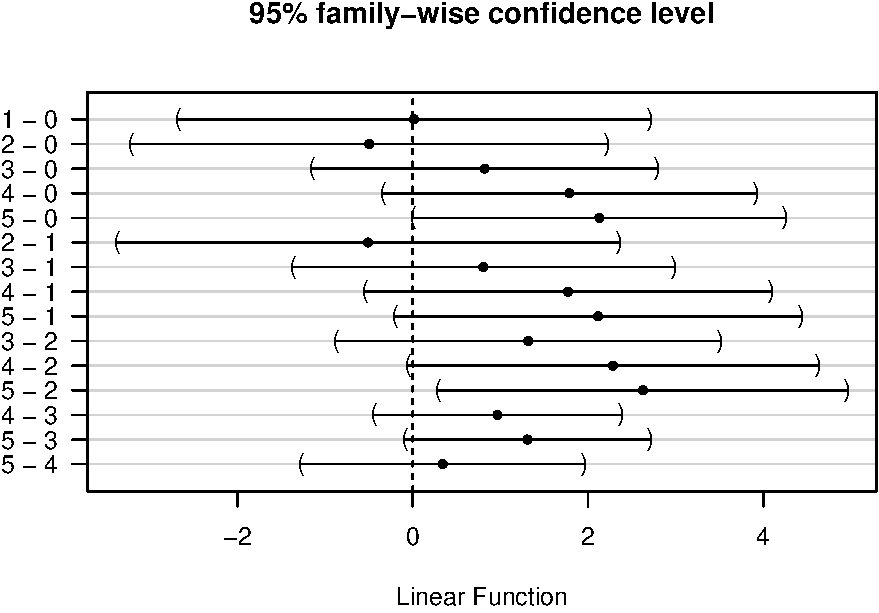
\includegraphics{PSY202A-Modeling-I.Heo_files/figure-latex/unnamed-chunk-99-1.pdf}

\begin{itemize}
\tightlist
\item
  Instead of post hoc comparison, researchers may have a priori contrasts from their research hypotheses. For example, researchers expect a linear trend in the impact of education on ACT score. The contrast coefficient of the linear trend for six groups can be created:
\end{itemize}

\begin{Shaded}
\begin{Highlighting}[]
\CommentTok{\# Contrast}
\NormalTok{ctr }\OtherTok{\textless{}{-}} \FunctionTok{matrix}\NormalTok{(}\FunctionTok{c}\NormalTok{(}\SpecialCharTok{{-}}\FloatTok{2.5}\NormalTok{, }\SpecialCharTok{{-}}\FloatTok{1.5}\NormalTok{, }\SpecialCharTok{{-}}\FloatTok{0.5}\NormalTok{, }\FloatTok{0.5}\NormalTok{, }\FloatTok{1.5}\NormalTok{, }\FloatTok{2.5}\NormalTok{), }\DecValTok{1}\NormalTok{, }\DecValTok{6}\NormalTok{)}
\end{Highlighting}
\end{Shaded}

\begin{itemize}
\tightlist
\item
  The polynomial contrast coefficient is based on Table A10 in Maxwell and Delaney (2004). The contrast is specified in a matrix where rows represent different contrasts and columns represent the coefficient of each group. The contrast can be evaluated using the glht function from the \texttt{multcomp} package:
\end{itemize}

\begin{Shaded}
\begin{Highlighting}[]
\CommentTok{\# Simultanoues tests for general linear hypotheses}
\NormalTok{linear }\OtherTok{\textless{}{-}} \FunctionTok{glht}\NormalTok{(model\_oaov, }\AttributeTok{linfct =} \FunctionTok{mcp}\NormalTok{(}\AttributeTok{education =}\NormalTok{ ctr))}
\FunctionTok{summary}\NormalTok{(linear)}
\end{Highlighting}
\end{Shaded}

\begin{verbatim}
## 
##   Simultaneous Tests for General Linear Hypotheses
## 
## Multiple Comparisons of Means: User-defined Contrasts
## 
## 
## Fit: aov(formula = ACT ~ education, data = dat)
## 
## Linear Hypotheses:
##        Estimate Std. Error t value Pr(>|t|)    
## 1 == 0    8.639      2.272   3.802 0.000156 ***
## ---
## Signif. codes:  0 '***' 0.001 '**' 0.01 '*' 0.05 '.' 0.1 ' ' 1
## (Adjusted p values reported -- single-step method)
\end{verbatim}

\begin{itemize}
\item
  The contrast is provided in the \texttt{linfct} argument. Because only one contrast is tested, the familywise error rate correction is not needed.
\item
  Next, all polynomial contrasts up to the fifth order are investigated for the difference in ACT between education levels:
\end{itemize}

\begin{Shaded}
\begin{Highlighting}[]
\CommentTok{\# Different contrasts as examples}
\NormalTok{linear }\OtherTok{\textless{}{-}} \FunctionTok{c}\NormalTok{(}\SpecialCharTok{{-}}\DecValTok{5}\NormalTok{, }\SpecialCharTok{{-}}\DecValTok{3}\NormalTok{, }\SpecialCharTok{{-}}\DecValTok{1}\NormalTok{, }\DecValTok{1}\NormalTok{, }\DecValTok{3}\NormalTok{, }\DecValTok{5}\NormalTok{)}
\NormalTok{quadratic }\OtherTok{\textless{}{-}} \FunctionTok{c}\NormalTok{(}\DecValTok{5}\NormalTok{, }\SpecialCharTok{{-}}\DecValTok{1}\NormalTok{, }\SpecialCharTok{{-}}\DecValTok{4}\NormalTok{, }\SpecialCharTok{{-}}\DecValTok{4}\NormalTok{, }\SpecialCharTok{{-}}\DecValTok{1}\NormalTok{, }\DecValTok{5}\NormalTok{)}
\NormalTok{cubic }\OtherTok{\textless{}{-}} \FunctionTok{c}\NormalTok{(}\SpecialCharTok{{-}}\DecValTok{5}\NormalTok{, }\DecValTok{7}\NormalTok{, }\DecValTok{4}\NormalTok{, }\SpecialCharTok{{-}}\DecValTok{4}\NormalTok{, }\SpecialCharTok{{-}}\DecValTok{7}\NormalTok{, }\DecValTok{5}\NormalTok{)}
\NormalTok{quartic }\OtherTok{\textless{}{-}} \FunctionTok{c}\NormalTok{(}\DecValTok{1}\NormalTok{, }\SpecialCharTok{{-}}\DecValTok{3}\NormalTok{, }\DecValTok{2}\NormalTok{, }\DecValTok{2}\NormalTok{, }\SpecialCharTok{{-}}\DecValTok{3}\NormalTok{, }\DecValTok{1}\NormalTok{)}
\NormalTok{quintic }\OtherTok{\textless{}{-}} \FunctionTok{c}\NormalTok{(}\SpecialCharTok{{-}}\DecValTok{1}\NormalTok{, }\DecValTok{5}\NormalTok{, }\SpecialCharTok{{-}}\DecValTok{10}\NormalTok{, }\DecValTok{10}\NormalTok{, }\SpecialCharTok{{-}}\DecValTok{5}\NormalTok{, }\DecValTok{1}\NormalTok{)}
\NormalTok{mctr }\OtherTok{\textless{}{-}} \FunctionTok{rbind}\NormalTok{(linear, quadratic, cubic, quartic, quintic)}
\end{Highlighting}
\end{Shaded}

\begin{itemize}
\tightlist
\item
  As mentioned above, the row of the contrast matrix represents different contrasts. The matrix of multiple contrasts can be used in the glht function:
\end{itemize}

\begin{Shaded}
\begin{Highlighting}[]
\CommentTok{\# Multiple testing}
\NormalTok{polynomial }\OtherTok{\textless{}{-}} \FunctionTok{glht}\NormalTok{(model\_oaov, }\AttributeTok{linfct =} \FunctionTok{mcp}\NormalTok{(}\AttributeTok{education =}\NormalTok{ mctr))}
\FunctionTok{summary}\NormalTok{(polynomial, }\AttributeTok{test=}\FunctionTok{adjusted}\NormalTok{(}\AttributeTok{type =} \StringTok{"bonferroni"}\NormalTok{))}
\end{Highlighting}
\end{Shaded}

\begin{verbatim}
## 
##   Simultaneous Tests for General Linear Hypotheses
## 
## Multiple Comparisons of Means: User-defined Contrasts
## 
## 
## Fit: aov(formula = ACT ~ education, data = dat)
## 
## Linear Hypotheses:
##                Estimate Std. Error t value Pr(>|t|)    
## linear == 0      17.279      4.544   3.802  0.00078 ***
## quadratic == 0    7.546      4.928   1.531  0.63099    
## cubic == 0       -7.027      7.515  -0.935  1.00000    
## quartic == 0     -2.629      2.999  -0.877  1.00000    
## quintic == 0      6.442      8.793   0.733  1.00000    
## ---
## Signif. codes:  0 '***' 0.001 '**' 0.01 '*' 0.05 '.' 0.1 ' ' 1
## (Adjusted p values reported -- bonferroni method)
\end{verbatim}

\section{Factorial ANOVA}\label{factorial-anova}

\begin{itemize}
\tightlist
\item
  Shall we use a different dataset this time?
\end{itemize}

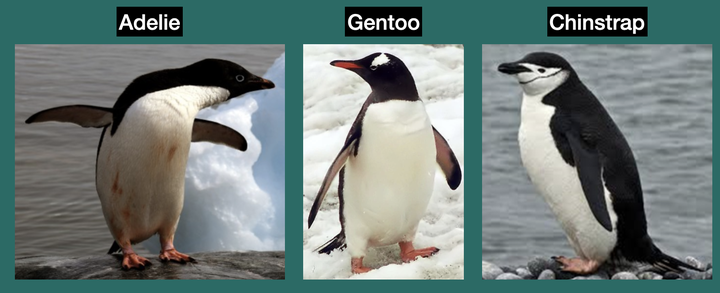
\includegraphics{./img/penguines.png}

\begin{itemize}
\item
  Here, assume we are interested in testing whether there are significant mean differences in body mass across the different species and sex levels.
\item
  There are three different types for the species variable and two levels for the sex variable.
\end{itemize}

\begin{Shaded}
\begin{Highlighting}[]
\CommentTok{\# Use penguins data}
\NormalTok{dat }\OtherTok{\textless{}{-}}\NormalTok{ penguins}

\CommentTok{\# Quick look at the data}
\FunctionTok{str}\NormalTok{(dat)}
\end{Highlighting}
\end{Shaded}

\begin{verbatim}
## tibble [344 x 8] (S3: tbl_df/tbl/data.frame)
##  $ species          : Factor w/ 3 levels "Adelie","Chinstrap",..: 1 1 1 1 1 1 1 1 1 1 ...
##  $ island           : Factor w/ 3 levels "Biscoe","Dream",..: 3 3 3 3 3 3 3 3 3 3 ...
##  $ bill_length_mm   : num [1:344] 39.1 39.5 40.3 NA 36.7 39.3 38.9 39.2 34.1 42 ...
##  $ bill_depth_mm    : num [1:344] 18.7 17.4 18 NA 19.3 20.6 17.8 19.6 18.1 20.2 ...
##  $ flipper_length_mm: int [1:344] 181 186 195 NA 193 190 181 195 193 190 ...
##  $ body_mass_g      : int [1:344] 3750 3800 3250 NA 3450 3650 3625 4675 3475 4250 ...
##  $ sex              : Factor w/ 2 levels "female","male": 2 1 1 NA 1 2 1 2 NA NA ...
##  $ year             : int [1:344] 2007 2007 2007 2007 2007 2007 2007 2007 2007 2007 ...
\end{verbatim}

\begin{Shaded}
\begin{Highlighting}[]
\FunctionTok{describe}\NormalTok{(dat)}
\end{Highlighting}
\end{Shaded}

\begin{verbatim}
##                   vars   n    mean     sd  median trimmed    mad    min    max
## species*             1 344    1.92   0.89    2.00    1.90   1.48    1.0    3.0
## island*              2 344    1.66   0.73    2.00    1.58   1.48    1.0    3.0
## bill_length_mm       3 342   43.92   5.46   44.45   43.91   7.04   32.1   59.6
## bill_depth_mm        4 342   17.15   1.97   17.30   17.17   2.22   13.1   21.5
## flipper_length_mm    5 342  200.92  14.06  197.00  200.34  16.31  172.0  231.0
## body_mass_g          6 342 4201.75 801.95 4050.00 4154.01 889.56 2700.0 6300.0
## sex*                 7 333    1.50   0.50    2.00    1.51   0.00    1.0    2.0
## year                 8 344 2008.03   0.82 2008.00 2008.04   1.48 2007.0 2009.0
##                    range  skew kurtosis    se
## species*             2.0  0.16    -1.73  0.05
## island*              2.0  0.61    -0.91  0.04
## bill_length_mm      27.5  0.05    -0.89  0.30
## bill_depth_mm        8.4 -0.14    -0.92  0.11
## flipper_length_mm   59.0  0.34    -1.00  0.76
## body_mass_g       3600.0  0.47    -0.74 43.36
## sex*                 1.0 -0.02    -2.01  0.03
## year                 2.0 -0.05    -1.51  0.04
\end{verbatim}

\begin{Shaded}
\begin{Highlighting}[]
\FunctionTok{summary}\NormalTok{(dat)}
\end{Highlighting}
\end{Shaded}

\begin{verbatim}
##       species          island    bill_length_mm  bill_depth_mm  
##  Adelie   :152   Biscoe   :168   Min.   :32.10   Min.   :13.10  
##  Chinstrap: 68   Dream    :124   1st Qu.:39.23   1st Qu.:15.60  
##  Gentoo   :124   Torgersen: 52   Median :44.45   Median :17.30  
##                                  Mean   :43.92   Mean   :17.15  
##                                  3rd Qu.:48.50   3rd Qu.:18.70  
##                                  Max.   :59.60   Max.   :21.50  
##                                  NA's   :2       NA's   :2      
##  flipper_length_mm  body_mass_g       sex           year     
##  Min.   :172.0     Min.   :2700   female:165   Min.   :2007  
##  1st Qu.:190.0     1st Qu.:3550   male  :168   1st Qu.:2007  
##  Median :197.0     Median :4050   NA's  : 11   Median :2008  
##  Mean   :200.9     Mean   :4202                Mean   :2008  
##  3rd Qu.:213.0     3rd Qu.:4750                3rd Qu.:2009  
##  Max.   :231.0     Max.   :6300                Max.   :2009  
##  NA's   :2         NA's   :2
\end{verbatim}

\begin{itemize}
\tightlist
\item
  For the ease of interpretation and implementation, I excluded penguins where the sex variable is missing:
\end{itemize}

\begin{Shaded}
\begin{Highlighting}[]
\CommentTok{\# Data engineering for exclusing cases where sex variable is missing}
\NormalTok{dat }\OtherTok{\textless{}{-}}\NormalTok{ dat }\SpecialCharTok{\%\textgreater{}\%} \FunctionTok{filter}\NormalTok{(}\SpecialCharTok{!}\FunctionTok{is.na}\NormalTok{(sex))}

\CommentTok{\# Quick look at the modified data}
\FunctionTok{str}\NormalTok{(dat)}
\end{Highlighting}
\end{Shaded}

\begin{verbatim}
## tibble [333 x 8] (S3: tbl_df/tbl/data.frame)
##  $ species          : Factor w/ 3 levels "Adelie","Chinstrap",..: 1 1 1 1 1 1 1 1 1 1 ...
##  $ island           : Factor w/ 3 levels "Biscoe","Dream",..: 3 3 3 3 3 3 3 3 3 3 ...
##  $ bill_length_mm   : num [1:333] 39.1 39.5 40.3 36.7 39.3 38.9 39.2 41.1 38.6 34.6 ...
##  $ bill_depth_mm    : num [1:333] 18.7 17.4 18 19.3 20.6 17.8 19.6 17.6 21.2 21.1 ...
##  $ flipper_length_mm: int [1:333] 181 186 195 193 190 181 195 182 191 198 ...
##  $ body_mass_g      : int [1:333] 3750 3800 3250 3450 3650 3625 4675 3200 3800 4400 ...
##  $ sex              : Factor w/ 2 levels "female","male": 2 1 1 1 2 1 2 1 2 2 ...
##  $ year             : int [1:333] 2007 2007 2007 2007 2007 2007 2007 2007 2007 2007 ...
\end{verbatim}

\begin{Shaded}
\begin{Highlighting}[]
\FunctionTok{describe}\NormalTok{(dat)}
\end{Highlighting}
\end{Shaded}

\begin{verbatim}
##                   vars   n    mean     sd median trimmed    mad    min    max
## species*             1 333    1.92   0.89    2.0    1.90   1.48    1.0    3.0
## island*              2 333    1.65   0.71    2.0    1.57   1.48    1.0    3.0
## bill_length_mm       3 333   43.99   5.47   44.5   43.98   6.97   32.1   59.6
## bill_depth_mm        4 333   17.16   1.97   17.3   17.19   2.22   13.1   21.5
## flipper_length_mm    5 333  200.97  14.02  197.0  200.36  16.31  172.0  231.0
## body_mass_g          6 333 4207.06 805.22 4050.0 4159.46 889.56 2700.0 6300.0
## sex*                 7 333    1.50   0.50    2.0    1.51   0.00    1.0    2.0
## year                 8 333 2008.04   0.81 2008.0 2008.05   1.48 2007.0 2009.0
##                    range  skew kurtosis    se
## species*             2.0  0.16    -1.72  0.05
## island*              2.0  0.62    -0.85  0.04
## bill_length_mm      27.5  0.04    -0.90  0.30
## bill_depth_mm        8.4 -0.15    -0.91  0.11
## flipper_length_mm   59.0  0.36    -0.98  0.77
## body_mass_g       3600.0  0.47    -0.75 44.13
## sex*                 1.0 -0.02    -2.01  0.03
## year                 2.0 -0.08    -1.49  0.04
\end{verbatim}

\begin{Shaded}
\begin{Highlighting}[]
\FunctionTok{summary}\NormalTok{(dat)}
\end{Highlighting}
\end{Shaded}

\begin{verbatim}
##       species          island    bill_length_mm  bill_depth_mm  
##  Adelie   :146   Biscoe   :163   Min.   :32.10   Min.   :13.10  
##  Chinstrap: 68   Dream    :123   1st Qu.:39.50   1st Qu.:15.60  
##  Gentoo   :119   Torgersen: 47   Median :44.50   Median :17.30  
##                                  Mean   :43.99   Mean   :17.16  
##                                  3rd Qu.:48.60   3rd Qu.:18.70  
##                                  Max.   :59.60   Max.   :21.50  
##  flipper_length_mm  body_mass_g       sex           year     
##  Min.   :172       Min.   :2700   female:165   Min.   :2007  
##  1st Qu.:190       1st Qu.:3550   male  :168   1st Qu.:2007  
##  Median :197       Median :4050                Median :2008  
##  Mean   :201       Mean   :4207                Mean   :2008  
##  3rd Qu.:213       3rd Qu.:4775                3rd Qu.:2009  
##  Max.   :231       Max.   :6300                Max.   :2009
\end{verbatim}

\subsection{How can we characterize this design?}\label{how-can-we-characterize-this-design}

\begin{itemize}
\item
  There are two factors in this study. The first factor is species, and the second factor is sex. Species has three levels (Adelie, Chinstrap, and Gentoo), and sex has two levels (female and male). In total, there are six combinations formed by the three levels of species and the two levels of sex, with penguins assigned to all six combinations. This indicates that the current study employs a \(3 \times 2\) factorial design. For this design, a two-way ANOVA should be conducted. The three null hypotheses being tested are as follows:
\item
  \(H_0\) (regarding species): Species does not have a significant main effect on body mass (group means on body mass across the three levels of species are not different).
\item
  \(H_0\) (regarding sex): Sex does not have a significant main effect on body mass (group means on body mass across the two levels of sex are not different).
\item
  \(H_0\) (regarding interaction): There is no significant interaction between species and sex on body mass.
\end{itemize}

\subsection{Cells means for the data}\label{cells-means-for-the-data}

\begin{Shaded}
\begin{Highlighting}[]
\CommentTok{\# Mean by groups in a wide format}
\NormalTok{dat.tab }\OtherTok{\textless{}{-}}\NormalTok{ dat }\SpecialCharTok{\%\textgreater{}\%} \FunctionTok{group\_by}\NormalTok{(species, sex) }\SpecialCharTok{\%\textgreater{}\%}
  \FunctionTok{summarise}\NormalTok{(}\AttributeTok{mean\_bodymass =} \FunctionTok{mean}\NormalTok{(body\_mass\_g)) }\SpecialCharTok{\%\textgreater{}\%}
  \FunctionTok{spread}\NormalTok{(sex, mean\_bodymass)}
\end{Highlighting}
\end{Shaded}

\begin{verbatim}
## `summarise()` has grouped output by 'species'. You can override using the
## `.groups` argument.
\end{verbatim}

\begin{Shaded}
\begin{Highlighting}[]
\CommentTok{\# Add the marginal means for species}
\NormalTok{dat.tab}\SpecialCharTok{$}\NormalTok{Means }\OtherTok{\textless{}{-}} \FunctionTok{rowMeans}\NormalTok{(dat.tab[}\DecValTok{2}\SpecialCharTok{:}\DecValTok{3}\NormalTok{])}

\CommentTok{\# Add the marginal means for sex}
\NormalTok{col\_means }\OtherTok{\textless{}{-}} \FunctionTok{c}\NormalTok{(}\FunctionTok{colMeans}\NormalTok{(dat.tab[}\DecValTok{2}\SpecialCharTok{:}\DecValTok{4}\NormalTok{]))}
\NormalTok{dat.tab }\OtherTok{\textless{}{-}} \FunctionTok{rbind}\NormalTok{(dat.tab, col\_means)}
\NormalTok{dat.tab}\SpecialCharTok{$}\NormalTok{species }\OtherTok{\textless{}{-}} \FunctionTok{c}\NormalTok{(}\StringTok{"Adelie"}\NormalTok{, }\StringTok{"Chinstrap"}\NormalTok{, }\StringTok{"Gentoo"}\NormalTok{, }\StringTok{"Means"}\NormalTok{)}

\CommentTok{\# Print the table}
\NormalTok{dat.tab}
\end{Highlighting}
\end{Shaded}

\begin{verbatim}
## # A tibble: 4 x 4
## # Groups:   species [4]
##   species   female  male Means
##   <chr>      <dbl> <dbl> <dbl>
## 1 Adelie     3369. 4043. 3706.
## 2 Chinstrap  3527. 3939. 3733.
## 3 Gentoo     4680. 5485. 5082.
## 4 Means      3859. 4489. 4174.
\end{verbatim}

\begin{itemize}
\item
  Can you understand the means by groups? In particular:

  \begin{itemize}
  \item
    Can you find any simple effect? (i.e., the effect of one IV at a specific level of the other IV)
  \item
    Can you find any main effect? (i.e., the average effect of the IV across the levels of all other IVs)
  \item
    Can you find any interaction effect? (i.e., the simple effects of one IV are not constant across all levels of the other IV; there is a differential effect)
  \end{itemize}
\end{itemize}

\subsection{Visualizing cell means}\label{visualizing-cell-means}

\begin{Shaded}
\begin{Highlighting}[]
\CommentTok{\# Jittered scatterplot with mean and SE}
\NormalTok{dat }\SpecialCharTok{\%\textgreater{}\%}
  \FunctionTok{ggplot}\NormalTok{(}\FunctionTok{aes}\NormalTok{(}\AttributeTok{x =}\NormalTok{ species, }\AttributeTok{y =}\NormalTok{ body\_mass\_g)) }\SpecialCharTok{+}
  \FunctionTok{facet\_wrap}\NormalTok{(}\SpecialCharTok{\textasciitilde{}}\NormalTok{sex) }\SpecialCharTok{+}
  \FunctionTok{stat\_summary}\NormalTok{(}\AttributeTok{fun.dat =} \StringTok{"mean\_se"}\NormalTok{, }\AttributeTok{geom =} \StringTok{"errorbar"}\NormalTok{, }\AttributeTok{wide =} \FloatTok{0.5}\NormalTok{) }\SpecialCharTok{+}
  \FunctionTok{stat\_summary}\NormalTok{(}\AttributeTok{fun.dat =} \StringTok{"mean\_se"}\NormalTok{, }\AttributeTok{geom =} \StringTok{"pointrange"}\NormalTok{) }\SpecialCharTok{+}
  \FunctionTok{geom\_jitter}\NormalTok{(}\AttributeTok{cex =} \FloatTok{1.5}\NormalTok{, }\AttributeTok{pch =} \FloatTok{1.0}\NormalTok{)}
\end{Highlighting}
\end{Shaded}

\begin{verbatim}
## Warning in stat_summary(fun.dat = "mean_se", geom = "errorbar", wide = 0.5):
## Ignoring unknown parameters: `fun.dat` and `wide`
\end{verbatim}

\begin{verbatim}
## Warning in stat_summary(fun.dat = "mean_se", geom = "pointrange"): Ignoring
## unknown parameters: `fun.dat`
\end{verbatim}

\begin{verbatim}
## No summary function supplied, defaulting to `mean_se()`
## No summary function supplied, defaulting to `mean_se()`
## No summary function supplied, defaulting to `mean_se()`
## No summary function supplied, defaulting to `mean_se()`
\end{verbatim}

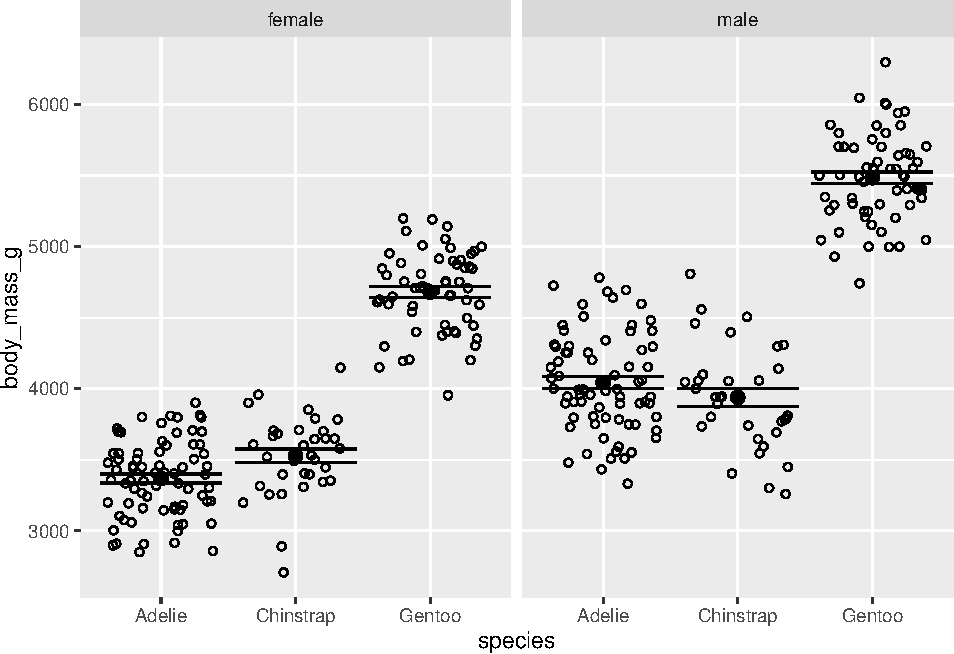
\includegraphics{PSY202A-Modeling-I.Heo_files/figure-latex/unnamed-chunk-107-1.pdf}

\begin{itemize}
\tightlist
\item
  What can you observe from the plot?
\end{itemize}

\subsection{Analysis}\label{analysis-1}

Let's conduct a two-way ANOVA to test whether there are mean differences in body mass across the different species and sex levels.

\begin{Shaded}
\begin{Highlighting}[]
\CommentTok{\# Perform a two{-}way ANOVA}
\CommentTok{\# Both of the code below do the same job}
\NormalTok{model\_taov }\OtherTok{\textless{}{-}} \FunctionTok{aov}\NormalTok{(body\_mass\_g }\SpecialCharTok{\textasciitilde{}}\NormalTok{ species }\SpecialCharTok{+}\NormalTok{ sex }\SpecialCharTok{+}\NormalTok{ species}\SpecialCharTok{:}\NormalTok{sex, }\AttributeTok{data =}\NormalTok{ dat)}
\DocumentationTok{\#\# The colon represents the interaction effect only}

\NormalTok{model\_taov }\OtherTok{\textless{}{-}} \FunctionTok{aov}\NormalTok{(body\_mass\_g }\SpecialCharTok{\textasciitilde{}}\NormalTok{ species}\SpecialCharTok{*}\NormalTok{sex, }\AttributeTok{data =}\NormalTok{ dat)}
\DocumentationTok{\#\# The asterisk represents the interaction effect and the main effect of each variable}
\DocumentationTok{\#\# (and all lower{-}order interactions)}

\CommentTok{\# Results}
\FunctionTok{summary}\NormalTok{(model\_taov)}
\end{Highlighting}
\end{Shaded}

\begin{verbatim}
##              Df    Sum Sq  Mean Sq F value   Pr(>F)    
## species       2 145190219 72595110 758.358  < 2e-16 ***
## sex           1  37090262 37090262 387.460  < 2e-16 ***
## species:sex   2   1676557   838278   8.757 0.000197 ***
## Residuals   327  31302628    95727                     
## ---
## Signif. codes:  0 '***' 0.001 '**' 0.01 '*' 0.05 '.' 0.1 ' ' 1
\end{verbatim}

\begin{Shaded}
\begin{Highlighting}[]
\CommentTok{\# Make the APA{-}style table}
\FunctionTok{apa.aov.table}\NormalTok{(model\_taov)}
\end{Highlighting}
\end{Shaded}

\begin{verbatim}
## 
## 
## ANOVA results using body_mass_g as the dependent variable
##  
## 
##      Predictor           SS  df           MS       F    p partial_eta2
##    (Intercept) 828480898.97   1 828480898.97 8654.65 .000             
##        species  60350016.02   2  30175008.01  315.22 .000          .66
##            sex  16613441.78   1  16613441.78  173.55 .000          .35
##  species x sex   1676556.74   2    838278.37    8.76 .000          .05
##          Error  31302628.28 327     95726.69                          
##  CI_90_partial_eta2
##                    
##          [.61, .69]
##          [.28, .41]
##          [.02, .09]
##                    
## 
## Note: Values in square brackets indicate the bounds of the 90% confidence interval for partial eta-squared
\end{verbatim}

\begin{Shaded}
\begin{Highlighting}[]
\CommentTok{\# Describe the result following the APA{-}style; but for reference ONLY!}
\FunctionTok{report}\NormalTok{(model\_taov)}
\end{Highlighting}
\end{Shaded}

\begin{verbatim}
## The ANOVA (formula: body_mass_g ~ species * sex) suggests that:
## 
##   - The main effect of species is statistically significant and large (F(2, 327)
## = 758.36, p < .001; Eta2 (partial) = 0.82, 95% CI [0.80, 1.00])
##   - The main effect of sex is statistically significant and large (F(1, 327) =
## 387.46, p < .001; Eta2 (partial) = 0.54, 95% CI [0.49, 1.00])
##   - The interaction between species and sex is statistically significant and
## small (F(2, 327) = 8.76, p < .001; Eta2 (partial) = 0.05, 95% CI [0.02, 1.00])
## 
## Effect sizes were labelled following Field's (2013) recommendations.
\end{verbatim}

\subsection{Can you explain to me how those results have been obtained?}\label{can-you-explain-to-me-how-those-results-have-been-obtained-1}

\begin{itemize}
\tightlist
\item
  I'll leave this as food for thought for you!
\end{itemize}

\subsection{How can we interpret the results?}\label{how-can-we-interpret-the-results-1}

\begin{itemize}
\item
  Let's use an alpha level of 0.05 as the significance threshold. According to the results, the p-value for species is lower than the significance level, indicating that species has a significant effect on body mass. In other words, the group means for body mass differ significantly across the three species.
\item
  The p-value for sex is also below the alpha level of 0.05, suggesting that sex has a significant effect on body mass. In other words, there are differences in body mass between female and male penguins.
\item
  Lastly, the p-value for the interaction between species and sex (denoted as species:sex in the output) is below the significance threshold. This indicates a significant interaction between species and sex. That is, the effect of species on body mass is not consistent across the levels of sex, as observed in the plot above.
\end{itemize}

\subsection{What to do with the interaction effect?}\label{what-to-do-with-the-interaction-effect}

\begin{itemize}
\item
  The interaction in the analysis suggests that it would be beneficial to examine the simple effects. The next step is to analyze the differences in body mass due to species within each level of sex.

  \begin{itemize}
  \item
    To do this, we will split the dataset and conduct a separate analysis for each level of sex.
  \item
    Importantly, to do this, we use the mean-squared-within (i.e., \(\text{MS}_{\text{within}}\)) from the full data to compute the F value, and then use the \texttt{pf} function to find the p-value.
  \item
    To control the overall Type I error rate, we will use an alpha level of 0.025 for each test.
  \end{itemize}
\end{itemize}

\subsubsection{What are you talking about, Ihnwhi\ldots?}\label{what-are-you-talking-about-ihnwhi}

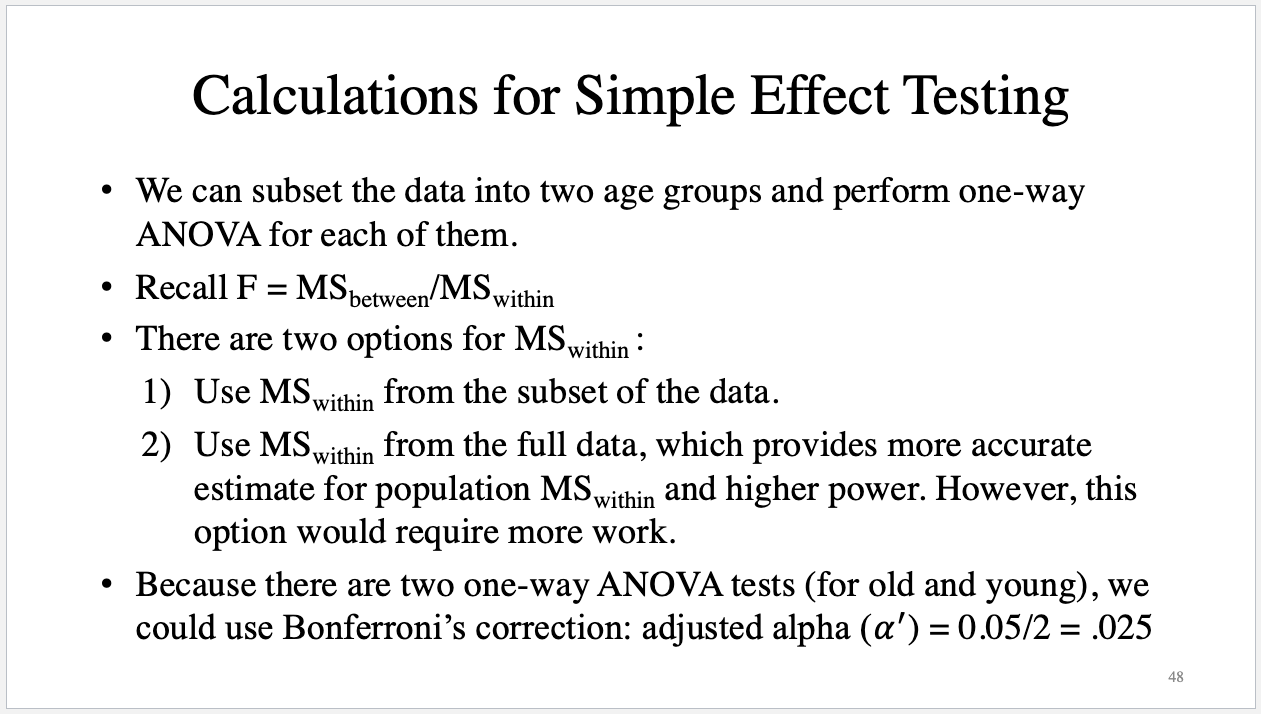
\includegraphics{./img/slide.png}

\begin{itemize}
\tightlist
\item
  Let's proceed with the analyses!
\end{itemize}

\begin{Shaded}
\begin{Highlighting}[]
\CommentTok{\# Split data}
\DocumentationTok{\#\# female}
\NormalTok{dat\_f }\OtherTok{\textless{}{-}} \FunctionTok{filter}\NormalTok{(dat, sex }\SpecialCharTok{==} \StringTok{"female"}\NormalTok{)}
\NormalTok{model\_taov\_f }\OtherTok{\textless{}{-}} \FunctionTok{aov}\NormalTok{(body\_mass\_g }\SpecialCharTok{\textasciitilde{}}\NormalTok{ species, }\AttributeTok{data =}\NormalTok{ dat\_f)}
\FunctionTok{summary}\NormalTok{(model\_taov\_f)}
\end{Highlighting}
\end{Shaded}

\begin{verbatim}
##              Df   Sum Sq  Mean Sq F value Pr(>F)    
## species       2 60350016 30175008   393.2 <2e-16 ***
## Residuals   162 12430757    76733                   
## ---
## Signif. codes:  0 '***' 0.001 '**' 0.01 '*' 0.05 '.' 0.1 ' ' 1
\end{verbatim}

\begin{Shaded}
\begin{Highlighting}[]
\CommentTok{\# MS\_between from the subset of data}
\NormalTok{MS\_b\_f }\OtherTok{\textless{}{-}} \FunctionTok{summary}\NormalTok{(model\_taov\_f)[[}\DecValTok{1}\NormalTok{]][}\DecValTok{1}\NormalTok{,}\DecValTok{3}\NormalTok{]}

\CommentTok{\# df\_between frmo the subset of data}
\NormalTok{df\_b\_f }\OtherTok{\textless{}{-}} \FunctionTok{summary}\NormalTok{(model\_taov\_f)[[}\DecValTok{1}\NormalTok{]][}\DecValTok{1}\NormalTok{,}\DecValTok{1}\NormalTok{]}

\CommentTok{\# MS\_within from the full data}
\NormalTok{MS\_w }\OtherTok{\textless{}{-}} \FunctionTok{summary}\NormalTok{(model\_taov)[[}\DecValTok{1}\NormalTok{]][}\DecValTok{4}\NormalTok{,}\DecValTok{3}\NormalTok{]}

\CommentTok{\# df\_within from the full data}
\NormalTok{df\_w }\OtherTok{\textless{}{-}} \FunctionTok{summary}\NormalTok{(model\_taov)[[}\DecValTok{1}\NormalTok{]][}\DecValTok{4}\NormalTok{,}\DecValTok{1}\NormalTok{]}

\CommentTok{\# Calculate the F{-}value}
\NormalTok{F\_f }\OtherTok{\textless{}{-}}\NormalTok{ MS\_b\_f}\SpecialCharTok{/}\NormalTok{MS\_w}

\CommentTok{\# Obtain the p{-}value}
\NormalTok{p\_f }\OtherTok{\textless{}{-}} \FunctionTok{pf}\NormalTok{(F\_f, }\AttributeTok{df1 =}\NormalTok{ df\_b\_f, }\AttributeTok{df2 =}\NormalTok{ df\_w, }\AttributeTok{lower.tail =} \ConstantTok{FALSE}\NormalTok{)}

\CommentTok{\# Make a statistical decision {-} Is p{-}value lower than the adjusted alpha?}
\NormalTok{p\_f }\SpecialCharTok{\textless{}} \FloatTok{0.025}
\end{Highlighting}
\end{Shaded}

\begin{verbatim}
## [1] TRUE
\end{verbatim}

\begin{itemize}
\item
  The results indicate that the p-value is lower than the adjusted alpha level of 0.025 based on Bonferroni's correction. This suggests that there are significant mean differences across the three levels of species when the level of sex is female.
\item
  We do the same for the subset of the data where the level of sex is male.
\end{itemize}

\begin{Shaded}
\begin{Highlighting}[]
\CommentTok{\# Split data}
\DocumentationTok{\#\# male}
\NormalTok{dat\_m }\OtherTok{\textless{}{-}} \FunctionTok{filter}\NormalTok{(dat, sex }\SpecialCharTok{==} \StringTok{"male"}\NormalTok{)}
\NormalTok{model\_taov\_m }\OtherTok{\textless{}{-}} \FunctionTok{aov}\NormalTok{(body\_mass\_g }\SpecialCharTok{\textasciitilde{}}\NormalTok{ species, }\AttributeTok{data =}\NormalTok{ dat\_m)}
\FunctionTok{summary}\NormalTok{(model\_taov\_m)}
\end{Highlighting}
\end{Shaded}

\begin{verbatim}
##              Df   Sum Sq  Mean Sq F value Pr(>F)    
## species       2 84728125 42364062   370.4 <2e-16 ***
## Residuals   165 18871872   114375                   
## ---
## Signif. codes:  0 '***' 0.001 '**' 0.01 '*' 0.05 '.' 0.1 ' ' 1
\end{verbatim}

\begin{Shaded}
\begin{Highlighting}[]
\CommentTok{\# MS\_between from the subset of data}
\NormalTok{MS\_b\_m }\OtherTok{\textless{}{-}} \FunctionTok{summary}\NormalTok{(model\_taov\_m)[[}\DecValTok{1}\NormalTok{]][}\DecValTok{1}\NormalTok{,}\DecValTok{3}\NormalTok{]}

\CommentTok{\# df\_between frmo the subset of data}
\NormalTok{df\_b\_m }\OtherTok{\textless{}{-}} \FunctionTok{summary}\NormalTok{(model\_taov\_m)[[}\DecValTok{1}\NormalTok{]][}\DecValTok{1}\NormalTok{,}\DecValTok{1}\NormalTok{]}

\CommentTok{\# MS\_within from the full data}
\NormalTok{MS\_w }\OtherTok{\textless{}{-}} \FunctionTok{summary}\NormalTok{(model\_taov)[[}\DecValTok{1}\NormalTok{]][}\DecValTok{4}\NormalTok{,}\DecValTok{3}\NormalTok{]}

\CommentTok{\# df\_within from the full data}
\NormalTok{df\_w }\OtherTok{\textless{}{-}} \FunctionTok{summary}\NormalTok{(model\_taov)[[}\DecValTok{1}\NormalTok{]][}\DecValTok{4}\NormalTok{,}\DecValTok{1}\NormalTok{]}

\CommentTok{\# Calculate the F{-}value}
\NormalTok{F\_m }\OtherTok{\textless{}{-}}\NormalTok{ MS\_b\_m}\SpecialCharTok{/}\NormalTok{MS\_w}

\CommentTok{\# Obtain the p{-}value}
\NormalTok{p\_m }\OtherTok{\textless{}{-}} \FunctionTok{pf}\NormalTok{(F\_m, }\AttributeTok{df1 =}\NormalTok{ df\_b\_m, }\AttributeTok{df2 =}\NormalTok{ df\_w, }\AttributeTok{lower.tail =} \ConstantTok{FALSE}\NormalTok{)}

\CommentTok{\# Make a statistical decision {-} Is p{-}value lower than the adjusted alpha?}
\NormalTok{p\_m }\SpecialCharTok{\textless{}} \FloatTok{0.025}
\end{Highlighting}
\end{Shaded}

\begin{verbatim}
## [1] TRUE
\end{verbatim}

\begin{itemize}
\tightlist
\item
  Similarly, the p-value is lower than the adjusted alpha level of 0.025 based on Bonferroni's correction. This indicates that there are significant mean differences across the three levels of species when the level of sex is male.
\end{itemize}

\subsection{This time, let's use pairwise comparison with Tukey's HSD to elaborate on the results of F.}\label{this-time-lets-use-pairwise-comparison-with-tukeys-hsd-to-elaborate-on-the-results-of-f.}

\begin{itemize}
\tightlist
\item
  We will use the \texttt{lsmeans()} function to perform pairwise comparisons based on Tukey's HSD.
\end{itemize}

\begin{Shaded}
\begin{Highlighting}[]
\CommentTok{\# Pairwise comparison}
\FunctionTok{lsmeans}\NormalTok{(model\_taov, pairwise }\SpecialCharTok{\textasciitilde{}}\NormalTok{ species, }\AttributeTok{by =} \StringTok{"sex"}\NormalTok{, }\AttributeTok{adjust =} \StringTok{"tukey"}\NormalTok{)}
\end{Highlighting}
\end{Shaded}

\begin{verbatim}
## $lsmeans
## sex = female:
##  species   lsmean   SE  df lower.CL upper.CL
##  Adelie      3369 36.2 327     3298     3440
##  Chinstrap   3527 53.1 327     3423     3632
##  Gentoo      4680 40.6 327     4600     4760
## 
## sex = male:
##  species   lsmean   SE  df lower.CL upper.CL
##  Adelie      4043 36.2 327     3972     4115
##  Chinstrap   3939 53.1 327     3835     4043
##  Gentoo      5485 39.6 327     5407     5563
## 
## Confidence level used: 0.95 
## 
## $contrasts
## sex = female:
##  contrast           estimate   SE  df t.ratio p.value
##  Adelie - Chinstrap     -158 64.2 327  -2.465  0.0377
##  Adelie - Gentoo       -1311 54.4 327 -24.088  <.0001
##  Chinstrap - Gentoo    -1153 66.8 327 -17.246  <.0001
## 
## sex = male:
##  contrast           estimate   SE  df t.ratio p.value
##  Adelie - Chinstrap      105 64.2 327   1.627  0.2357
##  Adelie - Gentoo       -1441 53.7 327 -26.855  <.0001
##  Chinstrap - Gentoo    -1546 66.2 327 -23.345  <.0001
## 
## P value adjustment: tukey method for comparing a family of 3 estimates
\end{verbatim}

\begin{itemize}
\item
  Can you understand the results? Focus on the \texttt{\$contrasts} section!
\item
  Can you expand on your results? Feel free to refer to the lecture slides for a template to guide your write-up.
\end{itemize}

\section{Regression analysis}\label{regression-analysis}

\begin{itemize}
\item
  \textbf{Purpose of Regression Analysis}: Regression analysis is a statistical method used to examine the relationship between a dependent variable (outcome) and one or more independent variables (predictors). It helps quantify the strength and direction of these relationships.
\item
  \textbf{Key Objective}: The primary goal is to model the relationship between variables, allowing researchers to explain variations in the dependent variable and make predictions about future or unobserved data points.
\item
  \textbf{Types of Regression}: Regression analysis comes in various forms, such as simple regression (one predictor), multiple regression (multiple predictors), and specialized models (e.g., logistic regression for binary outcomes or polynomial regression for nonlinear relationships).
\item
  \textbf{Assumptions and Applications}: Regression models rely on assumptions such as linearity, independence, homoscedasticity, and normality of residuals. It is widely applied in fields like psychology, economics, and engineering to analyze trends, test hypotheses, and predict outcomes. You will have a deeper understanding into the assumptions in PSY202B with Sarah!
\item
  \textbf{Tips When Programming}: Be sure to differentiate what is regression on others!
\end{itemize}

\subsection{Simple regression analysis}\label{simple-regression-analysis}

\begin{itemize}
\item
  A simple regression model is used to describe the relationship between two variables: an independent variable (IV) and a dependent variable (DV).
\item
  The research question addressed by simple regression is whether the IV has an effect on the DV. If a significant effect is found, the model can be used to predict DV values for new IV values.
\item
  Assuming a linear relationship between the two variables, the mathematical expression for a simple regression model is \(y_i = b_0 + b_1x_i + \varepsilon_i\), where \(b_0\) and \(b_1\) are the regression coefficients (intercept and slope, respectively), and \(\varepsilon_i\) represents the error term.
\item
  The DV must be a continuous variable, while the IV can be either continuous or categorical.

  \begin{itemize}
  \tightlist
  \item
    For example, one-way ANOVA is a special case of simple regression, where the IV is categorical.
  \end{itemize}
\end{itemize}

\subsubsection{Simple regression analysis with a continuous predictor}\label{simple-regression-analysis-with-a-continuous-predictor}

\begin{itemize}
\item
  Say our goal is to predict the ACT score using age through a simple regression analysis.
\item
  What would be the null hypothesis?
\end{itemize}

\begin{Shaded}
\begin{Highlighting}[]
\CommentTok{\# Use the sat{-}act data again}
\NormalTok{dat\_satact }\OtherTok{\textless{}{-}}\NormalTok{ sat.act}

\CommentTok{\# Simple regression analysis, with a continuous predictor}
\NormalTok{model\_reg\_s\_cont }\OtherTok{\textless{}{-}} \FunctionTok{lm}\NormalTok{(ACT }\SpecialCharTok{\textasciitilde{}}\NormalTok{ age, }\AttributeTok{data =}\NormalTok{ dat\_satact)}
\FunctionTok{summary}\NormalTok{(model\_reg\_s\_cont)}
\end{Highlighting}
\end{Shaded}

\begin{verbatim}
## 
## Call:
## lm(formula = ACT ~ age, data = dat_satact)
## 
## Residuals:
##      Min       1Q   Median       3Q      Max 
## -25.3454  -3.1874   0.4301   3.6546   7.9915 
## 
## Coefficients:
##             Estimate Std. Error t value Pr(>|t|)    
## (Intercept) 27.11035    0.52148  51.988  < 2e-16 ***
## age          0.05614    0.01910   2.939  0.00341 ** 
## ---
## Signif. codes:  0 '***' 0.001 '**' 0.01 '*' 0.05 '.' 0.1 ' ' 1
## 
## Residual standard error: 4.797 on 698 degrees of freedom
## Multiple R-squared:  0.01222,    Adjusted R-squared:  0.01081 
## F-statistic: 8.635 on 1 and 698 DF,  p-value: 0.003406
\end{verbatim}

\begin{itemize}
\tightlist
\item
  Can you understand the output and interpret the result?
\end{itemize}

\subsubsection{Simple regression analysis with a categorical predictor}\label{simple-regression-analysis-with-a-categorical-predictor}

\begin{itemize}
\tightlist
\item
  This time, say we would like to predict the ACT score using education through a simple regression analysis.
\end{itemize}

\begin{Shaded}
\begin{Highlighting}[]
\CommentTok{\# Simple regression analysis, with a continuous predictor}
\NormalTok{model\_reg\_s\_cate }\OtherTok{\textless{}{-}} \FunctionTok{lm}\NormalTok{(ACT }\SpecialCharTok{\textasciitilde{}} \FunctionTok{as.factor}\NormalTok{(education), }\AttributeTok{data =}\NormalTok{ dat\_satact)}
\FunctionTok{summary}\NormalTok{(model\_reg\_s\_cate)}
\end{Highlighting}
\end{Shaded}

\begin{verbatim}
## 
## Call:
## lm(formula = ACT ~ as.factor(education), data = dat_satact)
## 
## Residuals:
##      Min       1Q   Median       3Q      Max 
## -23.9773  -3.2945   0.5263   3.7055   9.0227 
## 
## Coefficients:
##                       Estimate Std. Error t value Pr(>|t|)    
## (Intercept)            27.4737     0.6319  43.480  < 2e-16 ***
## as.factor(education)1   0.0152     0.9513   0.016  0.98725    
## as.factor(education)2  -0.4964     0.9573  -0.519  0.60425    
## as.factor(education)3   0.8209     0.6943   1.182  0.23748    
## as.factor(education)4   1.7872     0.7511   2.379  0.01761 *  
## as.factor(education)5   2.1292     0.7488   2.844  0.00459 ** 
## ---
## Signif. codes:  0 '***' 0.001 '**' 0.01 '*' 0.05 '.' 0.1 ' ' 1
## 
## Residual standard error: 4.771 on 694 degrees of freedom
## Multiple R-squared:  0.02887,    Adjusted R-squared:  0.02187 
## F-statistic: 4.126 on 5 and 694 DF,  p-value: 0.001063
\end{verbatim}

\begin{itemize}
\tightlist
\item
  Can you notice something from the above results compared to what we did as below?
\end{itemize}

\begin{Shaded}
\begin{Highlighting}[]
\CommentTok{\# Perform a one{-}way ANOVA}
\NormalTok{model\_oaov }\OtherTok{\textless{}{-}} \FunctionTok{aov}\NormalTok{(ACT }\SpecialCharTok{\textasciitilde{}}\NormalTok{ education, }\AttributeTok{data =}\NormalTok{ dat\_satact)}

\CommentTok{\# Print the output}
\FunctionTok{summary}\NormalTok{(model\_oaov)}
\end{Highlighting}
\end{Shaded}

\begin{verbatim}
##              Df Sum Sq Mean Sq F value   Pr(>F)    
## education     1    390   389.9   17.14 3.89e-05 ***
## Residuals   698  15874    22.7                     
## ---
## Signif. codes:  0 '***' 0.001 '**' 0.01 '*' 0.05 '.' 0.1 ' ' 1
\end{verbatim}

\subsection{Multiple regression analysis}\label{multiple-regression-analysis}

\begin{itemize}
\tightlist
\item
  Multiple linear regression allows more than one IVs to predict the dependent variable (DV). To examine effects of multiple IVs on the DV, we can simply add IVs in the linear model, \(y_i = b_0 + b_1 x_{1i} + b_2 x_{2i} + \cdots + b_p x_{pi} + \varepsilon_i\).
\end{itemize}

\subsubsection{Multiple regression analysis with two continuous variables}\label{multiple-regression-analysis-with-two-continuous-variables}

\begin{itemize}
\item
  Say our goal is to predict the body mass of penguins using flipper length and bill depth through a multiple regression analysis.
\item
  What would be the null hypothesis?
\end{itemize}

\begin{Shaded}
\begin{Highlighting}[]
\CommentTok{\# Load data again}
\NormalTok{dat\_penguin }\OtherTok{\textless{}{-}}\NormalTok{ penguins}

\CommentTok{\# Multiple regression analysis}
\NormalTok{model\_reg\_m\_1 }\OtherTok{\textless{}{-}} \FunctionTok{lm}\NormalTok{(body\_mass\_g }\SpecialCharTok{\textasciitilde{}}\NormalTok{ flipper\_length\_mm }\SpecialCharTok{+}\NormalTok{ bill\_depth\_mm, }\AttributeTok{data =}\NormalTok{ dat\_penguin)}
\FunctionTok{summary}\NormalTok{(model\_reg\_m\_1)}
\end{Highlighting}
\end{Shaded}

\begin{verbatim}
## 
## Call:
## lm(formula = body_mass_g ~ flipper_length_mm + bill_depth_mm, 
##     data = dat_penguin)
## 
## Residuals:
##      Min       1Q   Median       3Q      Max 
## -1029.78  -271.45   -23.58   245.15  1275.97 
## 
## Coefficients:
##                    Estimate Std. Error t value Pr(>|t|)    
## (Intercept)       -6541.907    540.751 -12.098   <2e-16 ***
## flipper_length_mm    51.541      1.865  27.635   <2e-16 ***
## bill_depth_mm        22.634     13.280   1.704   0.0892 .  
## ---
## Signif. codes:  0 '***' 0.001 '**' 0.01 '*' 0.05 '.' 0.1 ' ' 1
## 
## Residual standard error: 393.2 on 339 degrees of freedom
##   (2 observations deleted due to missingness)
## Multiple R-squared:  0.761,  Adjusted R-squared:  0.7596 
## F-statistic: 539.8 on 2 and 339 DF,  p-value: < 2.2e-16
\end{verbatim}

\begin{itemize}
\tightlist
\item
  Can you understand the output and interpret the result?
\end{itemize}

\subsubsection{Model diagnostics for multiple regression analysis}\label{model-diagnostics-for-multiple-regression-analysis}

\begin{quote}
Trailer: Again, much more in Sarah's PSY202B!
\end{quote}

\begin{itemize}
\tightlist
\item
  For the purpose of diagnosing model assumptions, we can check four diagnostic plots: (1) residuals vs.~fitted, (2) normal Q-Q, (3) scale-loation, (4) Cook's distance, and (5) residuals vs.~leverage.
\end{itemize}

\begin{Shaded}
\begin{Highlighting}[]
\CommentTok{\# Model diagnostics using visual tools}
\FunctionTok{plot}\NormalTok{(model\_reg\_m\_1, }\AttributeTok{which =} \DecValTok{1}\NormalTok{)}
\end{Highlighting}
\end{Shaded}

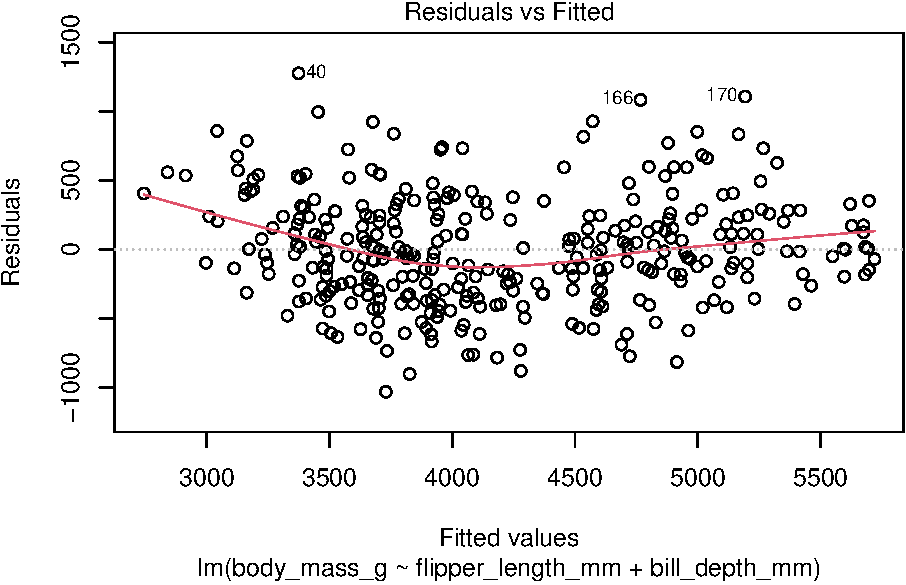
\includegraphics{PSY202A-Modeling-I.Heo_files/figure-latex/unnamed-chunk-118-1.pdf}

\begin{itemize}
\tightlist
\item
  A visual examination of the residuals vs.~fitted plot indicates that there is equal variance along the line of best fit (i.e., regression line). Therefore, the assumption of homoscedasticity is met. In addition, the points are randomly scattered across the place, and there are no discernible nonlinear trends. This means that the assumption of linearity is also met.
\end{itemize}

\begin{Shaded}
\begin{Highlighting}[]
\CommentTok{\# Model diagnostics using visual tools}
\FunctionTok{plot}\NormalTok{(model\_reg\_m\_1, }\AttributeTok{which =} \DecValTok{2}\NormalTok{)}
\end{Highlighting}
\end{Shaded}

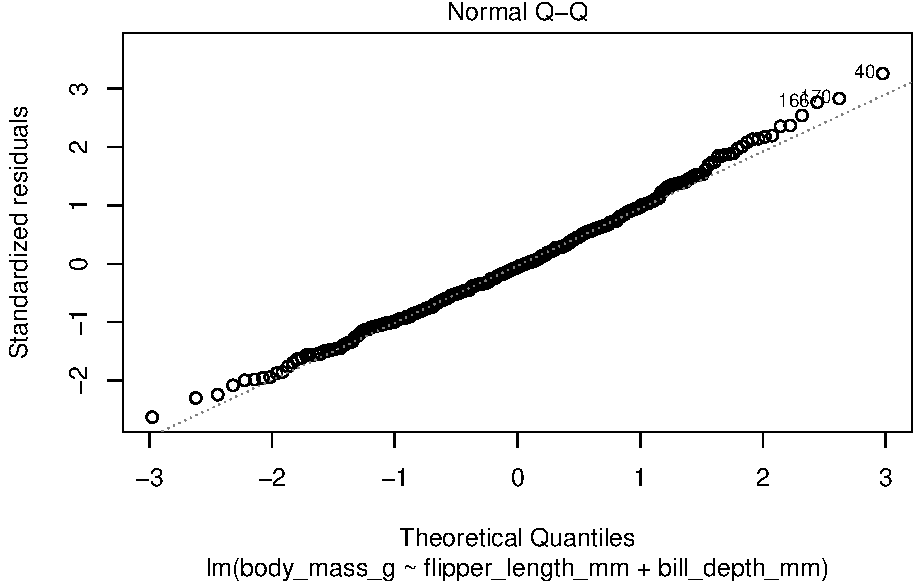
\includegraphics{PSY202A-Modeling-I.Heo_files/figure-latex/unnamed-chunk-119-1.pdf}

\begin{itemize}
\tightlist
\item
  The Q-Q plot shows that there is a slight deviation in the upper-right corner, but this is not severe and looks okay. Also, most of the data points hover around the normal line. Thus, the normality assumption is met.
\end{itemize}

\begin{Shaded}
\begin{Highlighting}[]
\CommentTok{\# Model diagnostics using visual tools}
\FunctionTok{plot}\NormalTok{(model\_reg\_m\_1, }\AttributeTok{which =} \DecValTok{3}\NormalTok{)}
\end{Highlighting}
\end{Shaded}

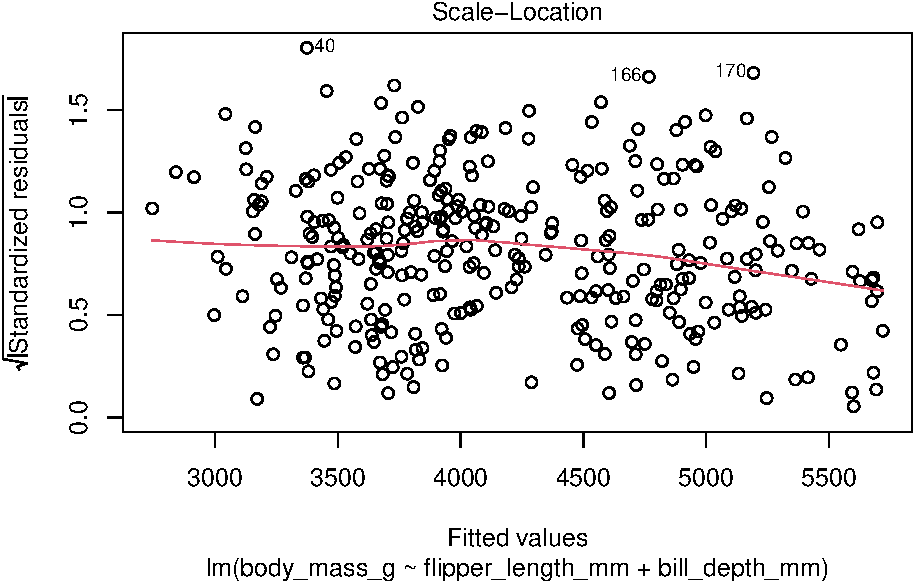
\includegraphics{PSY202A-Modeling-I.Heo_files/figure-latex/unnamed-chunk-120-1.pdf}

\begin{itemize}
\tightlist
\item
  The scale-location plot tells us whether the assumption of homoscedasticity is satisfied or violated. If a model satisfies this assumption, the points should ideally be equally spread around the red horizontal line. According to the plot, the red horizontal line is fairly flat, which suggests that the assumption of homoscedasticity is met. While observations such as 40, 166, and 170 deviate slightly more, I do not believe this indicates a severe violation of the homoscedasticity assumption.
\end{itemize}

\begin{Shaded}
\begin{Highlighting}[]
\CommentTok{\# Model diagnostics using visual tools}
\FunctionTok{par}\NormalTok{(}\AttributeTok{mfrow=}\FunctionTok{c}\NormalTok{(}\DecValTok{1}\NormalTok{,}\DecValTok{2}\NormalTok{))}
\FunctionTok{plot}\NormalTok{(model\_reg\_m\_1, }\AttributeTok{which =} \DecValTok{4}\NormalTok{)}
\FunctionTok{plot}\NormalTok{(model\_reg\_m\_1, }\AttributeTok{which =} \DecValTok{5}\NormalTok{)}
\end{Highlighting}
\end{Shaded}

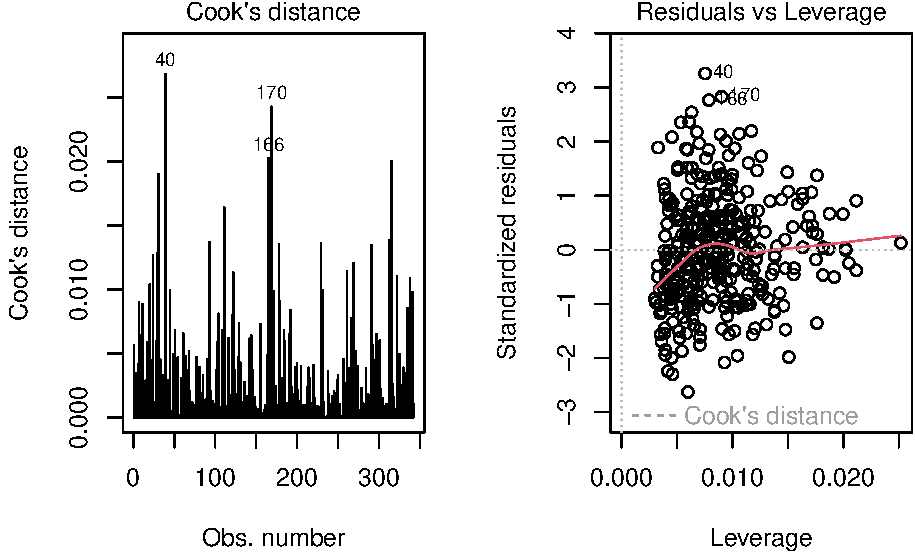
\includegraphics{PSY202A-Modeling-I.Heo_files/figure-latex/unnamed-chunk-121-1.pdf}

\begin{Shaded}
\begin{Highlighting}[]
\FunctionTok{par}\NormalTok{(}\AttributeTok{mfrow=}\FunctionTok{c}\NormalTok{(}\DecValTok{1}\NormalTok{,}\DecValTok{1}\NormalTok{))}
\end{Highlighting}
\end{Shaded}

\begin{itemize}
\item
  To diagnose the existence of influential points that can alter the results of the regression analysis upon the inclusion or exclusion of a value, I checked the Cook's distance plot and the residuals vs.~leverage plot. Cook's distance measures the influence of each data point on the fitted model. Larger values of Cook's distance, such as those greater than 0.5, indicate more influential points. According to the Cook's distance plot, values from observations 40, 170, 166 could be influential, so those values are worthy of closer scrutiny.
\item
  I checked the residuals vs.~leverage plot. According to this plot, observations with standardized residuals greater than 3 in absolute value are possible outliers. Indeed, there were three values whose absolute standardized residuals exceeded 3 (values from observations 40, 166, and 170), indicating the potential presence of outliers.
\item
  In sum, the assumption of no influential points is likely violated, at least for three specific observations. These values should be closely examined in the substantive research context.
\end{itemize}

\subsubsection{Multiple regression analysis with one continuous variable and one categorical variable}\label{multiple-regression-analysis-with-one-continuous-variable-and-one-categorical-variable}

\begin{itemize}
\item
  Say our goal is to predict the body mass of penguins using flipper length and sex through a multiple regression analysis.
\item
  We use female as a reference category (i.e., coded as 0), where male is coded as 1.
\item
  What would be the null hypothesis?
\end{itemize}

\begin{Shaded}
\begin{Highlighting}[]
\CommentTok{\# Quick data engineering}
\NormalTok{dat\_penguin }\OtherTok{\textless{}{-}}\NormalTok{ dat\_penguin }\SpecialCharTok{\%\textgreater{}\%}
  \FunctionTok{mutate}\NormalTok{(}\AttributeTok{sex\_dummy =} \FunctionTok{if\_else}\NormalTok{(sex }\SpecialCharTok{==} \StringTok{"male"}\NormalTok{, }\DecValTok{1}\NormalTok{, }\DecValTok{0}\NormalTok{))}

\CommentTok{\# Multiple regression analysis}
\NormalTok{model\_reg\_m\_2 }\OtherTok{\textless{}{-}} \FunctionTok{lm}\NormalTok{(body\_mass\_g }\SpecialCharTok{\textasciitilde{}}\NormalTok{ flipper\_length\_mm }\SpecialCharTok{+}\NormalTok{ sex\_dummy, }\AttributeTok{data =}\NormalTok{ dat\_penguin)}
\FunctionTok{summary}\NormalTok{(model\_reg\_m\_2)}
\end{Highlighting}
\end{Shaded}

\begin{verbatim}
## 
## Call:
## lm(formula = body_mass_g ~ flipper_length_mm + sex_dummy, data = dat_penguin)
## 
## Residuals:
##     Min      1Q  Median      3Q     Max 
## -910.28 -243.89   -2.94  238.85 1067.73 
## 
## Coefficients:
##                    Estimate Std. Error t value Pr(>|t|)    
## (Intercept)       -5410.300    285.798 -18.931  < 2e-16 ***
## flipper_length_mm    46.982      1.441  32.598  < 2e-16 ***
## sex_dummy           347.850     40.342   8.623 2.78e-16 ***
## ---
## Signif. codes:  0 '***' 0.001 '**' 0.01 '*' 0.05 '.' 0.1 ' ' 1
## 
## Residual standard error: 355.9 on 330 degrees of freedom
##   (11 observations deleted due to missingness)
## Multiple R-squared:  0.8058, Adjusted R-squared:  0.8047 
## F-statistic: 684.8 on 2 and 330 DF,  p-value: < 2.2e-16
\end{verbatim}

\begin{itemize}
\tightlist
\item
  Can you understand the output and interpret the result?
\end{itemize}

  \bibliography{book.bib,packages.bib}

\end{document}
